% !Mode:: "TeX:UTF-8"
%# -*- coding:utf-8 -*-

%% 南京大学学位论文的示例文档
%% 作者:njuhan: https://github.com/njuHan
%% 源模版repo: https://github.com/njuHan/njuthesis-nju-thesis-template

\documentclass[macfonts,master,oneside]{njuthesis}
%% 审阅模式很重要,命令是下方使用的/blind
%% njuthesis 文档类的可选参数有:
%%   winfonts, linuxfonts, macfonts, adobefonts winfonts 选项使得文档使用Windows 系统提供的字体;linuxfonts 选项使得文档使用Linux 系统提供的字体;macfonts 选项使得文档使用Mac 系统提供的字体;adobefonts 选项使得文档使用Adobe提供的OTF中文字体(需自行下载安转)
%%   phd/master/bachelor 选择博士/硕士/学士论文
%%   twoside 或 oneside 指定排版的文档为双面打印或单面打印格式(twoside会使得chapter 章节从奇数页开始,即纸张的正面开始,因此会出现一些空白的页面)
%%   nobackinfo 取消封二页导师签名信息。注意,按照南大的规定,是需要签名页的。



%%%%%%%%%%%%%%%%%%%%%%%%%%%%%%%%%%%%%%%%%%%%%%%%%%%%%%%%%%%%%%%%%%%%%%%%%%%%%%%
% set up labelformat and labelsep for subfigure 详见: http://www.latexstudio.net/archives/8652.html
\captionsetup[subfigure]{labelformat=simple, labelsep=space}

%%%%%%%%%%%%%%%%%%%%%%%%%%%%%%%%%%%%%%%%%%%%%%%%%%%%%%%%%%%%%%%%%%%%%%%%%%%%%%%
% 设置《国家图书馆封面》的内容,仅博士论文才需要填写

% 设置论文按照《中国图书资料分类法》的分类编号
%\classification{0175.2}
% 设置论文按照《国际十进分类法UDC》的分类编号
% 该编号可在下述网址查询:http://www.udcc.org/udcsummary/php/index.php?lang=chi
%\udc{004.72}
% 国家图书馆封面上的论文标题第一行,不可换行。此属性可选,默认值为通过\title设置的标题。
%\nlctitlea{论文标题第一行}
% 国家图书馆封面上的论文标题第二行,不可换行。此属性可选,默认值为空白。
%\nlctitleb{论文标题第二行}
% 国家图书馆封面上的论文标题第三行,不可换行。此属性可选,默认值为空白。
%\nlctitlec{}
% 导师的单位名称及地址
%\supervisorinfo{南京大学计算机科学与技术系~~南京市汉口路22号~~210093}
% 答辩委员会主席
%\chairman{张三丰~~教授}
% 第一位评阅人
%\reviewera{阳顶天~~教授}
% 第二位评阅人
%\reviewerb{张无忌~~副教授}
% 第三位评阅人
%\reviewerc{黄裳~~教授}
% 第四位评阅人
%\reviewerd{郭靖~~研究员}


%%%%%%%%%%%%%%%%%%%%%%%%%%%%%%%%%%%%%%%%%%%%%%%%%%%%%%%%%%%%%%%%%%%%%%%%%%%%%%%
% 设置论文的中文封面


% % 单行论文标题,不可换行
\title{}

% 如果论文标题过长,可以分两行,第一行用\titlea{}定义,第二行用\titleb{}定义,
% 使用以下3行:
%\title{} %用于覆盖单行标题内容为空
%\titlea{长标题第一行}  %第一行标题写这里
%\titleb{长标题第二行用于长标题换行} %第二行标题写这里
% 注意: \title 不能都注释,它用于控制标题选择双行还是单行。\title{}如果内容为空,则编译\titlea{},titleb{}双行标题,否则编译单行标题


% 论文作者姓名
\author{张富利}
% 论文作者联系电话
\telphone{18851751795}
% 论文作者电子邮件地址
\email{MG1932016@smail.nju.edu.cn}
% 论文作者学生证号
\studentnum{MG1932016}
% 论文作者入学年份(年级)
\grade{2019}
% 论文作者毕业年份(届), 出版授权书的学位年度
\graduateyear{2022}
% 导师姓名职称
\supervisor{张贺~~教授}
% 导师的联系电话
\supervisortelphone{}
% 论文作者的学科与专业方向
\major{软件工程}
% 论文作者的研究方向
\researchfield{DevOps、区块链}
% 论文作者所在院系的中文名称
\department{软件学院}
% 论文作者所在学校或机构的名称。此属性可选,默认值为``南京大学''。
\institute{南京大学}
% 论文的提交日期,需设置年、月、日。
\submitdate{xxxx年 xx 月 xx 日}
% 论文的答辩日期,需设置年、月、日。
\defenddate{xxxx年 xx 月 xx 日}
% 论文的定稿日期,需设置年、月、日。
% 此属性可选,若注释\date{},则默认值为最后一次编译时的日期,精确到日。
% \date{2019年5月20日}

%%%%%%%%%%%%%%%%%%%%%%%%%%%%%%%%%%%%%%%%%%%%%%%%%%%%%%%%%%%%%%%%%%%%%%%%%%%%%%%
% 设置论文的英文封面

% 论文的英文标题,不可换行
\englishtitle{}
\englishabstracttitlea{Modeling Support Method and Tool for}
\englishabstracttitleb{ Domain-Driven Design}
% 论文作者姓名的拼音
\englishauthor{Fuli Zhang}
% 导师姓名职称的英文
\englishsupervisor{Professor~~He Zhang}
% 论文作者学科与专业的英文名
\englishmajor{Software Engineering}
% 论文作者所在院系的英文名称
\englishdepartment{Software Institute}
% 论文作者所在学校或机构的英文名称。此属性可选,默认值为``Nanjing University''。
\englishinstitute{Nanjing University}
% 论文完成日期的英文形式,它将出现在英文封面下方。需设置年、月、日。日期格式使用美国的日期
% 格式,即``Month day, year'',其中``Month''为月份的英文名全称,首字母大写;``day''为
% 该月中日期的阿拉伯数字表示;``year''为年份的四位阿拉伯数字表示。
% 此属性可选,若注释掉\englishdate{},则默认值为最后一次编译时的日期。
% \englishdate{May 20, 2019}

%%%%%%%%%%%%%%%%%%%%%%%%%%%%%%%%%%%%%%%%%%%%%%%%%%%%%%%%%%%%%%%%%%%%%%%%%%%%%%%
% 设置论文的中文摘要

% 设置中文摘要页面的论文标题及副标题的第一行。
% 此属性可选,其默认值为使用|\title|命令所设置的论文标题
%\abstracttitlea{标题第一行}
% 设置中文摘要页面的论文标题及副标题的第二行。
% 此属性可选,其默认值为空白
%\abstracttitleb{标题第二行用于长标题换行}

%%%%%%%%%%%%%%%%%%%%%%%%%%%%%%%%%%%%%%%%%%%%%%%%%%%%%%%%%%%%%%%%%%%%%%%%%%%%%%%
% 设置论文的英文摘要

% 设置英文摘要页面的论文标题及副标题的第一行。
% 此属性可选,其默认值为使用|\englishtitle|命令所设置的论文标题
%\englishabstracttitlea{englishabstracttitlea}
% 设置英文摘要页面的论文标题及副标题的第二行。
% 此属性可选,其默认值为空白
%\englishabstracttitleb{nglishabstracttitleb}

%%%%%%%%%%%%%%%%%%%%%%%%%%%%%%%%%%%%%%%%%%%%%%%%%%%%%%%%%%%%%%%%%%%%%%%%%%%%%%
%% 盲审命令,空白字段设置请看 .cls文件 \newcommand*{\blind}
%% 此外,请按照盲审要求自行去掉个人简历、致谢等页面中的个人信息
%%**********************!!!非常重要的盲审命令,送审前必选!!!****************
% \blind
%%**********************!!!非常重要的盲审命令,送审前必选!!!****************

%%%%%%%%%%%%%%%%%%%%%%%%%%%%%%%%%%%%%%%%%%%%%%%%%%%%%%%%%%%%%%%%%%%%%%%%%%%%%%%
\begin{document}

%%%%%%%%%%%%%%%%%%%%%%%%%%%%%%%%%%%%%%%%%%%%%%%%%%%%%%%%%%%%%%%%%%%%%%%%%%%%%%%

% 制作国家图书馆封面(博士学位论文才需要)
%\makenlctitle
% 制作中文封面
\maketitle
% 制作英文封面
\makeenglishtitle

%%%%%%%%%%%%%%%%%%%%%%%%%%%%%%%%%%%%%%%%%%%%%%%%%%%%%%%%%%%%%%%%%%%%%%%%%%%%%%%
% 开始前言部分
\frontmatter

\begin{abstract}
  领域驱动设计是一种针对复杂业务流程的软件设计方法,
  它可以帮助架构师和软件开发人员提炼业务流程和构建复杂软件系统。
  近年来,
  越来越多的团队将领域驱动设计应用到大型分布式系统的设计与实现中。

  然而,作为领域驱动设计的核心内容,战术建模的应用却存在诸多问题与挑战。
  其一,战术建模模式的实践过程仍缺少标准且统一的规范,
  使得实践者无法准确地使用这些模式建模业务流程;
  其二,战术建模实践过程所缺少的规范,
  也使得开发人员和架构设计人员在使用这些建模模式时具有不同的理解,
  从而带来了一系列项目团队沟通问题;
  其三,现有的大多数建模平台对领域建模过程的支持仍不完善,
  极大地阻碍了领域战术建模的应用。

  为了解决上述问题与挑战,本文首先调研了现阶段有关领域驱动设计战术建模的理论文献,
  对具有相关实践经验的从业者进行访谈,
  提炼出一系列面向战术建模过程的实践规范作为战术建模指南。
  所提炼的建模指南包含一系列战术建模中使用到的战术模式、这些战术模式的属性、
  使用时机与实现技术。
  然后,基于UML扩展机制定义标准的领域驱动设计战术建模元模型作为战术建模语言。
  上述建模指南和战术建模语言共同组成本文所提出的战术建模支持方法。
  最后,基于所提出的战术建模支持方法,
  本文还实现了一个可视化战术建模工具DDDD(Draw for Domain-Driven Design),
  该工具支持标准化的战术建模、对建模结果的验证、复用以及扩展,
  帮助实践者更规范地进行战术建模。

  本文采用案例研究对提出的建模支持方法及工具进行验证。
  结果表明本文提出的战术建模支持方法及工具,
  能够帮助领域驱动设计的实践者开展更规范化的战术建模过程,
  从而解决战术建模实践过程缺少规范带来的一系列挑战,
  一定程度上促进了战术建模的应用。
	% 同时应该注意到,空白页是故意留白,以便章节开头能够出现在偶数页。
	% 中文关键词。关键词之间用中文全角分号隔开,末尾无标点符号。
	\keywords{领域驱动设计;战术建模;建模工具;特定领域建模语言}
\end{abstract}

%%%%%%%%%%%%%%%%%%%%%%%%%%%%%%%%%%%%%%%%%%%%%%%%%%%%%%%%%%%%%%%%%%%%%%%%%%%%%%%
% 论文的英文摘要
\begin{englishabstract}
  As a software design approach for complex business process, Domain-Driven Design (DDD) enables architects and developers building complex software system.
  In recent years, more and more teams have applied DDD to the design and implementation of large-scale distributed systems.

  However, as the core means of DDD, 
  tactical modeling are facing many challenges in its application.
  Firstly, the practicing process of tactical modeling patterns still lacks standard and unified specifications,
   making it hard for practitioners to use these patterns to model business processes accurately; 
  secondly, the lack of specifications also makes developers and architects have different understandings when using the modeling patterns,
   leading to a series of communication problems in project team; 
   thirdly, most of the existing modeling platforms have incomplete support for the tactical modeling process, 
   severely impeding the application of DDD.


  In order to solve the aforementioned challenges, 
  this thesis first reviews theoretical literature on tactical modeling,
   then interviews practitioners with relevant practical experience, 
  and finally extracts a series of practical specifications for the tactical modeling process.
   As a guide for tactical modeling, the specifications contain a series of tactical patterns used in tactical modeling, 
   their attributes, time of using, and implementation techniques. 
   Furthermore, the standard tactical modeling metamodel is defined based on UML profile mechanism, as a tactical modeling language. 
   The above modeling guide and tactical modeling language together constitute the tactical modeling support method proposed in this thesis. 
   Based on the proposed method, this thesis also implements a visual tactical modeling tool called Draw for Domain-Driven Design, or DDDD. 
   The tool supports standardized tactical modeling, verification, reuse and extension of modeling results to help practitioners develop tactical modeling in a more standardized way.


  This thesis uses case studies to verify the proposed modeling support method and tool. 
  Results show that the proposed method and tool can help DDD practitioners to conduct a more standardized tactical modeling process, 
  thus solving the challenges caused by lack of specification in the tactical modeling process, 
  and promoting the application of tactical modeling to a certain extent.
  
  \englishkeywords{Domain-driven design, Tactical modeling, Modeling tool, Domain-specific modeling language}
\end{englishabstract}

%%%%%%%%%%%%%%%%%%%%%%%%%%%%%%%%%%%%%%%%%%%%%%%%%%%%%%%%%%%%%%%%%%%%%%%%%%%%%%%
% 论文的前言,应放在目录之前,中英文摘要之后,一般不需要
%
%\begin{preface}
%
%在过去的40年中,手写中文文本领域识别(HCTR)取得了很大的进展[1,2]。
%
%\vspace{1cm}
%\begin{flushright}
%饶安逸\\
%2018年5月15日于南大仙林
%\end{flushright}
%
%\end{preface}

%%%%%%%%%%%%%%%%%%%%%%%%%%%%%%%%%%%%%%%%%%%%%%%%%%%%%%%%%%%%%%%%%%%%%%%%%%%%%%%
% 生成论文目录
\tableofcontents

%%%%%%%%%%%%%%%%%%%%%%%%%%%%%%%%%%%%%%%%%%%%%%%%%%%%%%%%%%%%%%%%%%%%%%%%%%%%%%%
% 生成插图清单。如无需插图清单则可注释掉下述语句。
\listoffigures

%%%%%%%%%%%%%%%%%%%%%%%%%%%%%%%%%%%%%%%%%%%%%%%%%%%%%%%%%%%%%%%%%%%%%%%%%%%%%%%
% 生成附表清单。如无需附表清单则可注释掉下述语句。
\listoftables

%%%%%%%%%%%%%%%%%%%%%%%%%%%%%%%%%%%%%%%%%%%%%%%%%%%%%%%%%%%%%%%%%%%%%%%%%%%%%%%
% 开始正文部分
\mainmatter

%%%%%%%%%%%%%%%%%%%%%%%%%%%%%%%%%%%%%%%%%%%%%%%%%%%%%%%%%%%%%%%%%%%%%%%%%%%%%%%
% 学位论文的正文应以《绪论》作为第一章,本模板是按照自身功能模块组织的,并非论文中的章节安排


\chapter{绪论}

\section{研究背景及意义}

区块链(Blockchain)是一种按照时间顺序将数据区块以链条的方式组成的特定数据结构,被视为一个分布式的共享账本和数据库。它能够使用户无需相互信任与可信第三方的条件下完成可信的价值传输\cite{SurveyofEnterpriseBlockchains}。作为区块链2.0 的以太坊\footnotemark[1]\footnotetext[1]{\href{http://github.com/ethereum/wiki/wiki/White-Paper/}{以太坊白皮书}}重新将智能合约描述为图灵完备的、部署于区块链网络中合同条款代码。这意味着传统的合同条款可以进入实体计算机中,且在区块链网络去中心化、不可伪造、不可篡改的特性下严格执行。区块链推进了人与企业之间和线上与线下之间的全方面互联,其被成为下一代的新型生产关系。随着区块链的快速发展, 智能合约极大地丰富和扩展了区块链应用场景。它们为供应链、金融等传统领域带来重大变革, 已经快速渗入到人们生活的方方面面。

与此同时, 云原生(Cloud native)作为一种基于云的基础之上的软件架构思想,以及基于云进行软件开发实践的一组方法论。因其弹性和分布式的优势成为当今流行的软件服务模式。云原生技术有利于各组织在公有云、私有云和混合云等新型动态环境中, 构建和运行可弹性扩展的应用, 借助平台的全面自动化能力, 跨多云构建微服务, 持续交付部署业务生产系统。

{\footnotesize
\begin{longtable}[h]{m{100pt} m{50pt} m{50pt} m{50pt} m{50pt}}
    \caption[主要公有云的BaaS平台]{主要公有云的BaaS平台} \label{major_BaaS_platforms} \\
        \toprule  
        \textbf{BaaS平台}&\textbf{Ethereum}&\textbf{Quorum}&\textbf{Corda}&\textbf{Fabric}\\
        \hline
        
        AWS&Y&Y&Y&Y\\

        Azure&Y&Y&Y&Y\\

        IBM& & & &Y\\

        阿里云区块链服务&Y& & &Y\\

        腾讯云区块链服务TBaaS& & & &Y\\

        华为云区块链服务BCS& & & &Y\\
        \bottomrule
    \end{longtable}
}

区块链即服务(Blockchain as a Service, 简称BaaS)则是基于云原生技术体系的一种构建、管理、托管和运维区块链网络及其应用的云服务平台\cite{onik2019performance}。BaaS支持将任何企业级区块链实施到云环境,而无需任何IT专业知识。这大大降低了区块链技术的使用门槛, 是促使区块链技术更广泛、更深入地渗透到各个行业和企业的催化剂, 其市值预计从2018年的6.23亿美元猛增2023年的150亿美元\footnotemark[1]\footnotetext[1]{\href{https://www.reportbuyer.com/product/5486837/global-blockchain-as-a-service-market.html}{Global Blockchain-as-a-Service Market 2018-2022}}。其中, 云厂商提供了大多数的BaaS平台\cite{KuernetesbasedFabricChaincodeManagementAndHihgAvailabilityTechnology}, 如表\ref{major_BaaS_platforms}所示, 其底层区块链支撑技术大多数选择IBM开源的跨企业级联盟链Hyperledger Fabric, 这也是本文选择Hyperledger Fabric的原因。


% 挑战
BaaS基于云的弹性可伸缩的能力屏蔽了底层区块链技术, 为上层去中心化应用的开发运维人员提供便捷的构建区块链网络等功能。然而, “Each coin has two sides”, 当前BaaS平台的发展尤其是底层的区块链基础设施的建设依旧存在诸多挑战。

首先, 基础商业化应用工具并不完善\footnotemark[2]\footnotetext[2]{\href{http://www.caict.ac.cn/kxyj/qwfb/ztbg/202107/P020210726503897354430.pdf}{区块链基础设施研究报告(2021年)}}。BaaS平台发展还处于初级阶段, 商业运行模式仍处在探索阶段。由于BaaS平台研发投入大, 目前市场上存在如AWS、IBM、阿里云区块链服务等多种BaaS平台解决方案, 这些BaaS平台计费高昂\footnotemark[3]\footnotetext[3]{\href{https://help.aliyun.com/document_detail/107710.html?spm=5176.14107623.commonbuy2container.1.59523b20xmyuNf}{阿里云区块链服务BaaS规格与定价}}并且与其他云服务捆绑销售。传统的企业业务或已存在稳定合作的云服务商, 使用不同云服务商的合作伙伴就需要跨云部署, 由于缺乏统一的顶层规划, 各云厂商的BaaS导致不同应用底层异构形成技术、信息孤岛, 存在不可复用的跨解决方案的资源和工具, 这导致了基于多云的网络\cite{DBLP:conf/coins/GerritsKKFV21}, 给跨云部署带来了诸多问题。同时, BaaS平台几乎都由互联网云服务巨头企业把控, 可用性限制通常会迫使其他企业为来自各种云提供商的基础设施即服务(Infrastructure as a Service, 简称IaaS)付费, 最终行业马太效应明显\cite{KuernetesbasedFabricChaincodeManagementAndHihgAvailabilityTechnology}。

其次, BaaS平台利用云能力对区块链基础设施赋能乏力。作为一种广泛部署的技术, 云计算是实施区块链技术的合适目标。然而, 区块链与云原生两种技术都相对不成熟, 但两者的集成可能会在技术方面产生新的复杂性\cite{onik2019performance}。行业缺少既定的标准或最佳实践范例, 各云厂商的BaaS解决方案基本都采取已有的开源解决方案, 业务同质化严重。他们 仅提供一种基于开源区块链平台的自动部署管理方案, 未深入到区块链与云基础设施的底层, 问题仍然在于如何使区块链和云兼容\cite{gai2020blockchain}, 区块链服务比常规云服务更复杂, 有许多未解决的问题需要回答。自动化脚本部署并不是有效的云化方式, 浪费了云原生技术的潜力。例如除区块链网络自动部署外, 在数据存储备份及可扩展性方面, 传统自动化部署方案无法利用云的弹性伸缩能力性且随着交易数量的增加, 区块数据最终会占满磁盘空间, 出现存储膨胀问题。区块链的数据可扩展性受到了的限制, 需要结合云的能力寻找数据备份、升级及可扩展性的方法。区块链如何和云原生快速深度结合, 利用原生伸缩性、可移植性和高可用性价值来提供“高质量”的区块链服务, 是当前仍然遗留的挑战。

% 意义、愿景
针对上述问题, 本文选择面向联盟链场景开源框架Hyperledger Fabric和Kubernetes提出了一种基于Hyperledger Fabric的区块链云化框架, 具体工作如图\ref{framework_tool}所示。该框架通过对Fabric网络中的Ca、Orderer、Peer组件进行抽象适配并利用Kubernetes Operator对其进行完整生命周期管理。本框架利用原生Kubernetes安全性、可扩展性等机制使用户通过专家提供的领域知识对Fabric网络获得类似云的自我管理。此外, 本文还实现了基于区块链云化框架的原型工具, 支持更简单、更原生的管理Fabric网络。

\begin{figure}[h] %figure环境,h默认参数是可以浮动,不是固定在当前位置。如果要不浮动,你就可以使用大写float宏包的H参数,固定图片在当前位置,禁止浮动。
    \centering %使图片居中显示
    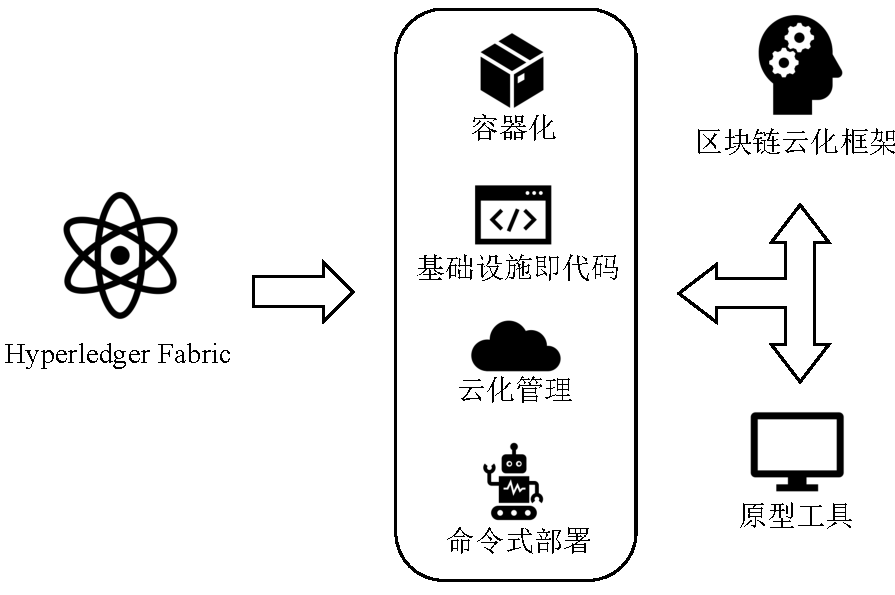
\includegraphics[width=0.7\textwidth]{FIGs/chapter1/framework_tool.pdf} %中括号中的参数是设置图片充满文档的大小,你也可以使用小数来缩小图片的尺寸。
    \caption{区块链云化框架及其原型工具} %caption是用来给图片加上图题的
    \label{framework_tool} %这是添加标签,方便在文章中引用图片。
\end{figure}%figure环境

\section{研究现状}

由于区块链智能合约的无法删除、修改、历史可追溯、去中心化、严格执行等特点, 越来越多的研究人员想挖掘区块链的潜能, 将区块链的能力应用到各种应用场景。McCorry等人\cite{mccorry2017smart}将区块链应用在电子投票领域, 实现了一个基于以太坊的去中心化互联网公开投票协议,公开投票网络是一种自助协议, 每个选民都控制着自己投票的隐私, 只有在所有人都参与的情况下才会被破坏, 这是第一个实现的不依赖任何可信的权威机构来计数和保护选民隐私的去中心化应用。Chang和Chen\cite{chang2020blockchain}在供应链领域进行了系统文献综述,表明传统的供应链活动涉及多个中介、信任和性能问题,利用区块链的潜力可以更好地扰乱供应链运作性能、分布式治理和过程自动化。Zhang和Wen\cite{zhang2017iot}提出了一种物联网电子商务模型,旨在重新设计传统电子商务模型中的许多元素,并借助区块链和智能合约技术在物联网上实现智能财产和付费数据的交易。Leka等人\cite{leka2019systematic}相信区块链技术将是下一个技术革命,同时表明区块链研究现阶段在物联网\cite{christidis2016blockchains}、医疗、教育、政府各个领域都有涉及。

目前, 去中心化应用逐步从概念验证阶段转变为工程化、商业化阶段。由于区块链的复杂性给网络的构建以及智能合约的部署、运维工作带来了严重的时间成本。在去中心化应用价值交付过程中, 存在对于区块链底层技术的易用性、部署效率、安全性等多方面的挑战。研究人员在区块链基础设施与云原生结合方面都开始了一定的探索, 除了利用区块链的特性提升云的能力外\cite{DBLP:journals/comcom/XieZZWH21}\cite{DBLP:conf/smartcloud/SunWY20}\cite{8457813}, 研究人员也都期望利用云的特性自动化地构建出易于弹性扩展、高可用的区块链平台。

% 学术
% 应用场景 BaaS平台往云上迁移
在学术研究方面, 研究人员在探究如何有效利用云平台来部署区块链平台。Gerrits等人\cite{DBLP:conf/coins/GerritsKKFV21}在Kubernetes中部署了分布式账本Hyperledger Sawtooth\footnotemark[1]\footnotetext[1]{\href{https://github.com/hyperledger/sawtooth-core}{Hyperledger Sawtooth github地址}}, 并运行了一个用例。他们旨在探讨该用例在真实场景云部署中的可行性和可扩展性。Liang等人\cite{liangeduchain}针对教育领域数据共享和信息欺骗的问题构建了一个高可用的教育联盟区块链平台, 并实现了基于Kubernetes的Fabric部署, 实现了将链码纳入Kubernetes环境管理的目标。然而, Wan等人\cite{wan2018novel}指出当前主流的BaaS提供商通常采用API进行用户访问, 或者简单地将区块链应用迁移到云, 这会侵蚀不可信的机制并带来锁定风险。他们随后提出了一种新的服务范式来克服现有BaaS的局限性。基于Hyperledger的实施表明, 该范式可以缓解当前BaaS对区块链特征的侵蚀。在云原生底层基础设施方面研究人员关注与区块链结合的Kubernetes调度问题。才\cite{caili2018}在Kubernetes上面对PBFT和区块链的本身特性提出了静态调度和自适应算法。Shi等人\cite{9582270}为了解决云端现实PoS区块链工作负载的高效调度问题, 首次在云计算中设计和实现了基于Kubernetes的解决PoS区块链应用程序迁移成本的系统, 最大限度地减少了使用的Kubernetes工作节点数量以降低总体费用,而且还提出了一种高性能的Kubernetes调度方案HPKS以最大限度地利用工作节点进行在线pod管理。

% 工业界
相比于学术研究, 工业领域的探索更加注重自动化实践。Hyperledger Cello\footnotemark[1]\footnotetext[1]{\href{https://github.com/hyperledger/cello}{Hyperledger Cello github地址}}支持在多种底层基础设施上从头快速构建BaaS平台, 提供管理区块链网络的生命周期、自定义区块链网络配置等功能帮助人们以更高效的方式使用和管理区块链。Hyperledger Cello当前阶段重点关注在Docker安装, 对于Kubernetes支持方面的仍处在相对初级阶段, 配置项简单灵活性不足且老旧。Blockchain Automation Framework\footnotemark[2]\footnotetext[2]{\href{https://github.com/nikoturin/blockchain-automation-framework}{Blockchain Automation Framework github地址}}提供了一个自动化框架, 利用Ansible\footnotemark[3]\footnotetext[3]{\href{https://github.com/ansible/ansible}{Ansible github地址}}以及Helm\footnotemark[4]\footnotetext[4]{\href{https://github.com/helm/helm}{Helm github地址}}快速地、一致地将生产就绪的分布式账本技术(Distributed ledger technology, 简称DLT)平台部署到云基础设施。虽然, Blockchain Automation Framework提供了一个自动化框架将区块链平台部署于Kubernetes, 但本质上还是描述为一个需要希望远程主机执行命令的方案,或者一组IT程序运行的命令集合。这大大提升了自动化程度,但其远没有发挥Kubernetes的潜力。

% 总结
尽管学术界以及工业界目前已有一些关于区块链云化的探索与研究, 研究重点多为如何自动化地将区块链平台向云上迁移, 研究缺少构建支持云和区块链一体化的有效服务模型\cite{9582270}。

与此同时, 一部分研究利用Kubernetes operator方法将云底层的效率、灵活性等多方面优势拓展到多种领域。Kubernetes operator是将领域知识集成到Kubernetes API编排过程中的最新方法\cite{henning2021reproducible}。Huang等人\cite{huang2021fly}提出了一个轻量级的遥感大数据处理云原生框架。该框架利用Kubernetes operator融合Spark, 自动化配置Spark参数, 提升并行遥感图像融合算法的效率。Zhou等人\cite{zhou2021container}提出了Torque operator对高性能(High Performance Computing, 简称HPC)的负载进行管理, 利用容器化来提升HPC的效率及灵活性。除此之外, 在5G领域\cite{arouk20205g}\cite{wiranata2020automation}、医疗\cite{rouzbeh2020unified}等领域, Kubernetes operator也发挥出其强大的自动化与编排能力, 利用云原生的可迁移性、可伸缩性、安全性等特性进行赋能, 但在区块链领域的Kubernetes operator相关工作较少。


\section{本文主要研究工作}

% 首先,它通过自动化以前手动编写的大部分代码,消除了人为错误,提高了系统的生产率。用户现在可以只为操作员编写自定义资源
% 管理Ray群集需要一组复杂的操作和配置参数,这些操作和参数必须由领域专家执行和设置,群集才能正常运行。这些知识嵌入到KubeRay操作符中,以减轻Ray用户的群集管理负担,并将其转移到操作符本身
% 虽然fabric和Kubernetes形成了理想的匹配,但许多开发ML应用程序的科学家缺乏必要的Kubernetes专业知识,无法在Kubernetes上设置Ray群集,并监控、调试和操作在此类环境中运行的应用程序
% 使用预先打包并经过工厂测试的映像,以最少的时间部署集群,而不是按照几页的说明仔细配置系统



% 本文主要的研究工作分为以下三个方面:

% 1.围绕领域驱动设计的战术建模过程展开了理论调研,
% 从《领域驱动设计:软件核心复杂性应对之道》\cite{DBLP:books/daglib/0013521}和
% 《实现领域驱动设计》\cite{vernon2013implementing}两本著作中抽取了八种战术建模模式及其重要特征。
% 具体地,针对八种战术建模模式,
% 设计了调查问卷,与工业界具有领域驱动设计实战经验的架构师和开发人员展开访谈;
% 根据访谈结果,通过多次焦点小组讨论,
% 对八种战术建模模式及其重要特征进行验证和完善,
% 克服了理论脱离实际的问题。
% 最终得出一套战术建模指南,该指南包括战术建模模式、模式属性、使用时机以及实现技术。


% 2.基于上述理论基础,通过UML profile机制扩展UML元类,实例化战术建模语言。
% 战术建模语言描述了战术模式的构造型、必要属性、关联关系以及重要约束。
% 以UML中元类为基础,更符合软件设计中面向对象(Object-Oriented)的思想,
% 也更易于软件从业者接受和学习。以该元模型为基础的建模语言,更关注战术建模,
% 包含最贴合实践的规则和约束,建模效率更高。

% 3.实现了一个战术建模支持工具,
% 该工具对建模过程中使用的战术模式进行约束与规范性校验,
% 对建模结果进行多种格式的转化与存储,
% 还包含生成框架项目代码包等扩展功能。
% 对战术建模支持工具进行了功能测试,并使用该工具进行了战术建模案例研究,
% 结果表明该工具支持开发人员快速理解各种战术模式的重要特征和规则约束,
% 降低了使用战术建模的学习成本;
% 可以对建模结果进行验证并提示开发人员进行修改,规范化建模过程;
% 还具有将建模结果转化为多种格式文件和框架项目代码的功能,使建模结果更具有通用性。


% 上述战术建模指南、战术建模语言以及战术建模支持工具共同组成了本文研究工作的战术建模支持方法及工具。

\section{本文组织结构}

本文组织结构如下:

第一章~绪论。介绍了本文的研究背景及意义、国内外研究现状、工业界的主要探索以及本文主要的研究工作;

第二章~理论与技术支持。介绍区块链尤其是Hyperledger Fabric的相关理论和概念; 同时介绍云原生的基本概念发展历程, 并对云原生基础设施Kubernetes进行了详细介绍;

第三章~基于Hyperledger Fabric的区块链云化框架。介绍区块链基础设施的现状及挑战, 基于这些现状区块链云化框架应当具有的设计原则, 并详细介绍了本文提出的基于Hyperledger Fabric的区块链云化框架。

第四章~原型工具设计与实现。;

第五章~框架检验与评估。;

第六章~总结与展望。

\section{本章小节}


\chapter{理论与技术支持}

本章将介绍区块链及云原生相关概念和理论知识, 还将介绍本文区块链云化框架所涉及到的其他技术与工具。

\section{区块链技术}\label{section: blockchain}

\subsection{区块链基本概念}
区块链是以比特币等数字加密货币体系为核心支撑技术的一种全新的去中心化基础架构与分布式计算范式\cite{1016383}。区块链通常被被当作分布式账本, 具有去中心化、持久性、匿名性、不可篡改性、可追溯性的特点。

\begin{figure}[h] %figure环境,h默认参数是可以浮动,不是固定在当前位置。如果要不浮动,你就可以使用大写float宏包的H参数,固定图片在当前位置,禁止浮动。
    \centering %使图片居中显示
    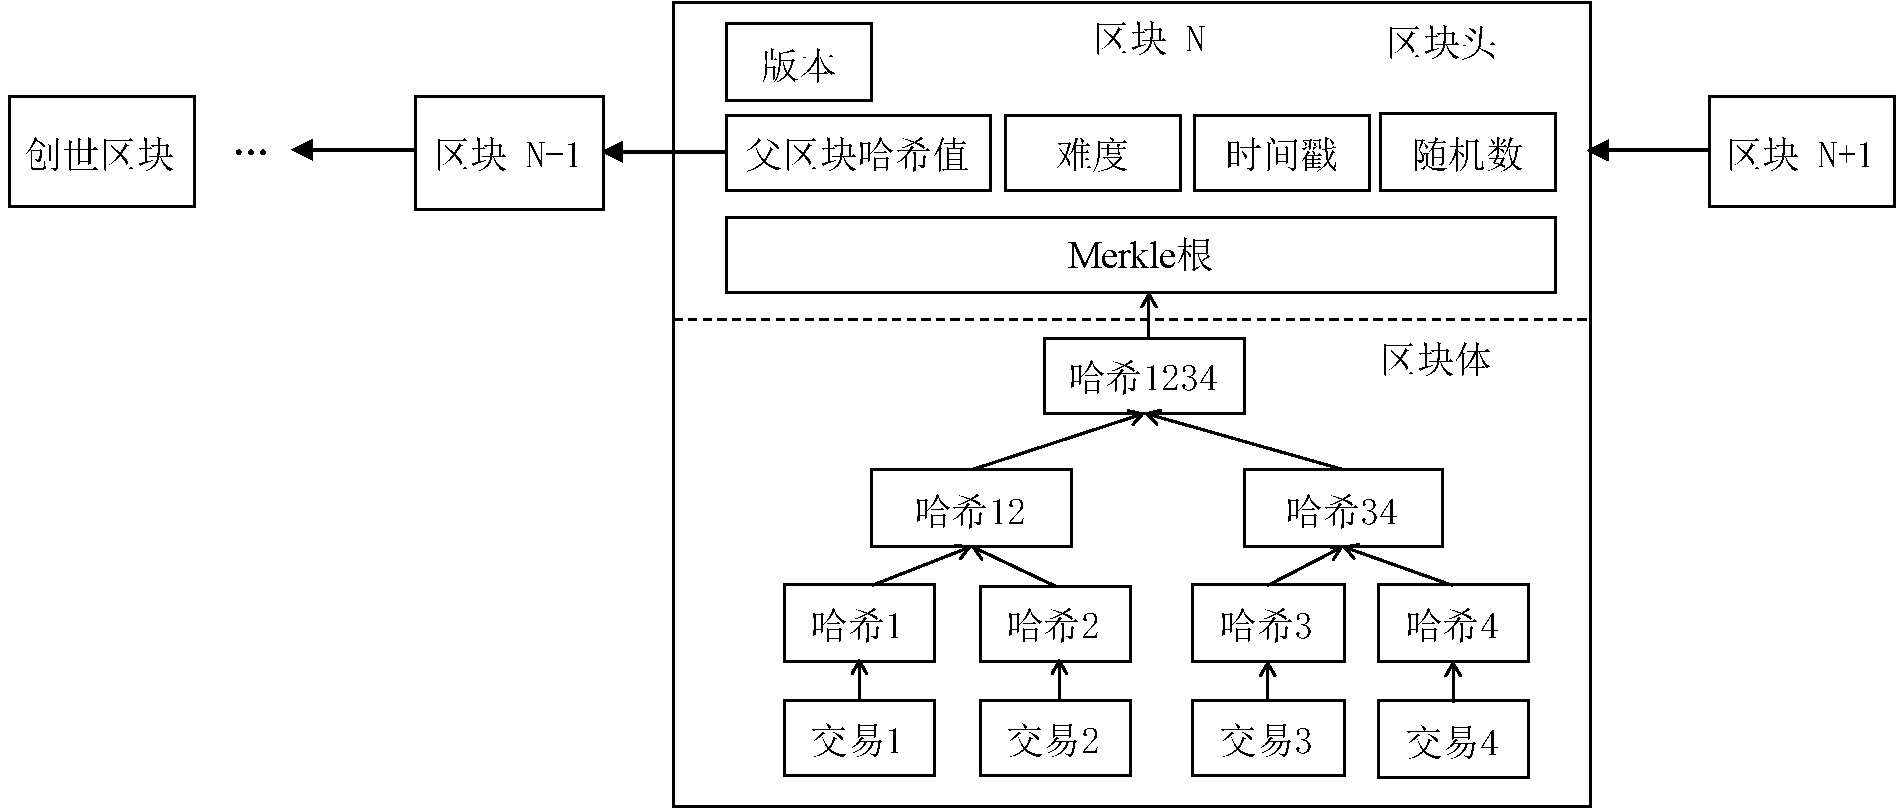
\includegraphics[width=1\textwidth]{FIGs/chapter2/blockchain_example.pdf} %中括号中的参数是设置图片充满文档的大小,你也可以使用小数来缩小图片的尺寸。
    \caption{区块链示例图} %caption是用来给图片加上图题的
    \label{blockchain_example} %这是添加标签,方便在文章中引用图片。
\end{figure}%figure环境

区块链典型示例如图\ref{blockchain_example}所示, 可以看作是一种按照时间顺序将数据区块以顺序相连的方式组合成的一种链式数据结构, 并以密码学方式保证的不可篡改和不可伪造的分布式账本。每个数据区块包含区块头(Block header)和区块体(Block body)两部分, 区块头主要用来存储本区块的一些相关属性, 区块体则用来存储真实的交易数据记录。区块头主要由三组数据组成, 第一组是父区块的哈希值, 用来将该区块与它的前一区块相连接; 第二组数据和矿工竞争挖矿有关, 即难度、时间戳和随机数(Nonce); 第三组是由区块体中计算出来的根哈希值, 即默克尔(Merkle)根。
区块体包括当前区块经过验证的、区块创建过程中生成的所有交易记录。这些记录通过默克尔树的哈希过程生成唯一的默克尔根并记入区块头。整个区块链的第一个区块称为创世区块(Genesis block)。
如果网络中大多数节点通过共识机制就新区块中交易的有效性和区块本身的有效性达成共识, 则可以将新区块添加到链中。

{\footnotesize
\begin{longtable}[h]{m{70pt} m{70pt} m{70pt} m{70pt}}
    \caption[区块链类型]{区块链类型} \label{blockchain_type} \\
        \toprule   
        &\textbf{公有区块链}&\textbf{私有区块链}&\textbf{联盟区块链}\\
        \hline
        准入限制&无&有&有\\
        
        读取者&任何人&仅限受邀用户&相关联用户\\
        
        写入者&任何人&获批参与者&获批参与者\\
        
        所属者&无&单一实体&多方实体\\
        
        交易速度&慢&快&快\\
        \bottomrule
    \end{longtable}
}

当前, 区块链分为公有区块链、联盟区块链和私有区块链。如表\ref{blockchain_type}所示, 公有链没有准入限制, 没有监管方可以组织参与, 任何人都可以参与共识, 常见的两种共识协议为工作量证明机制(Proof of work, 简称PoW)和权益证明机制(Proof of stake, 简称PoS)。由于任何人都可以自由加入, 因此公有链网络具有高度分布式的拓扑结构。但是, 公有链在安全性和性能方面也进行了权衡。公有链上的许多服务器遇到了扩展瓶颈, 吞吐量相对较弱; 与公有区块链的无准入限制形成鲜明对比的是, 私有区块链建立了准入规则, 规定谁可以查看和写入区块链。因为在控制方面有明确的层次结构, 私有链也不是去中心化系统。在某些私有链中, 具备安全模型的背景下,共识协议是多余的。因此在私有区块链中,不使用PoW并不会造成很严重的威胁, 因为每个参与者的身份都是已知的, 是手动进行管理的; 联盟区块链是介于公有链和私有链之间的,结合了两者的特征要素。在共识方面, 联盟链将少数同等权力的参与方视为验证者,而不是像公有链那样开放的系统, 让任何人都可以验证区块, 也不是像私有链那样, 通过一个封闭的系统, 只允许某一个实体来任命区块的生产者。对于从事各类活动的个人和企业来说,存在大量的区块链选择。即使在公有链、私有链和联盟链中,根据复杂性的不同,也会出现许多不同的用户体验。根据实际使用情况,企业可以选择最适合的链实现目标的产品。供应链、电商、医疗等需要彼此之间需要相互沟通的场景下, 联盟链可减轻私有链中交易对手的风险, 并且较少的节点数通常可使它们能够比公共链更有效率的运行, 因此通常选择联盟链。

\subsection{Hyperledger Fabric}
Hyperledger Fabric\footnotemark[1]\footnotetext[1]{\href{https://github.com/hyperledger/fabric}{Hyperledger Fabric}}是一种企业级联盟链解决方案, 因其可插拔模块化、可伸缩、可扩展的架构、多编程语言的智能合约受到业界广泛追捧。

\begin{figure}[h] %figure环境,h默认参数是可以浮动,不是固定在当前位置。如果要不浮动,你就可以使用大写float宏包的H参数,固定图片在当前位置,禁止浮动。
    \centering %使图片居中显示
    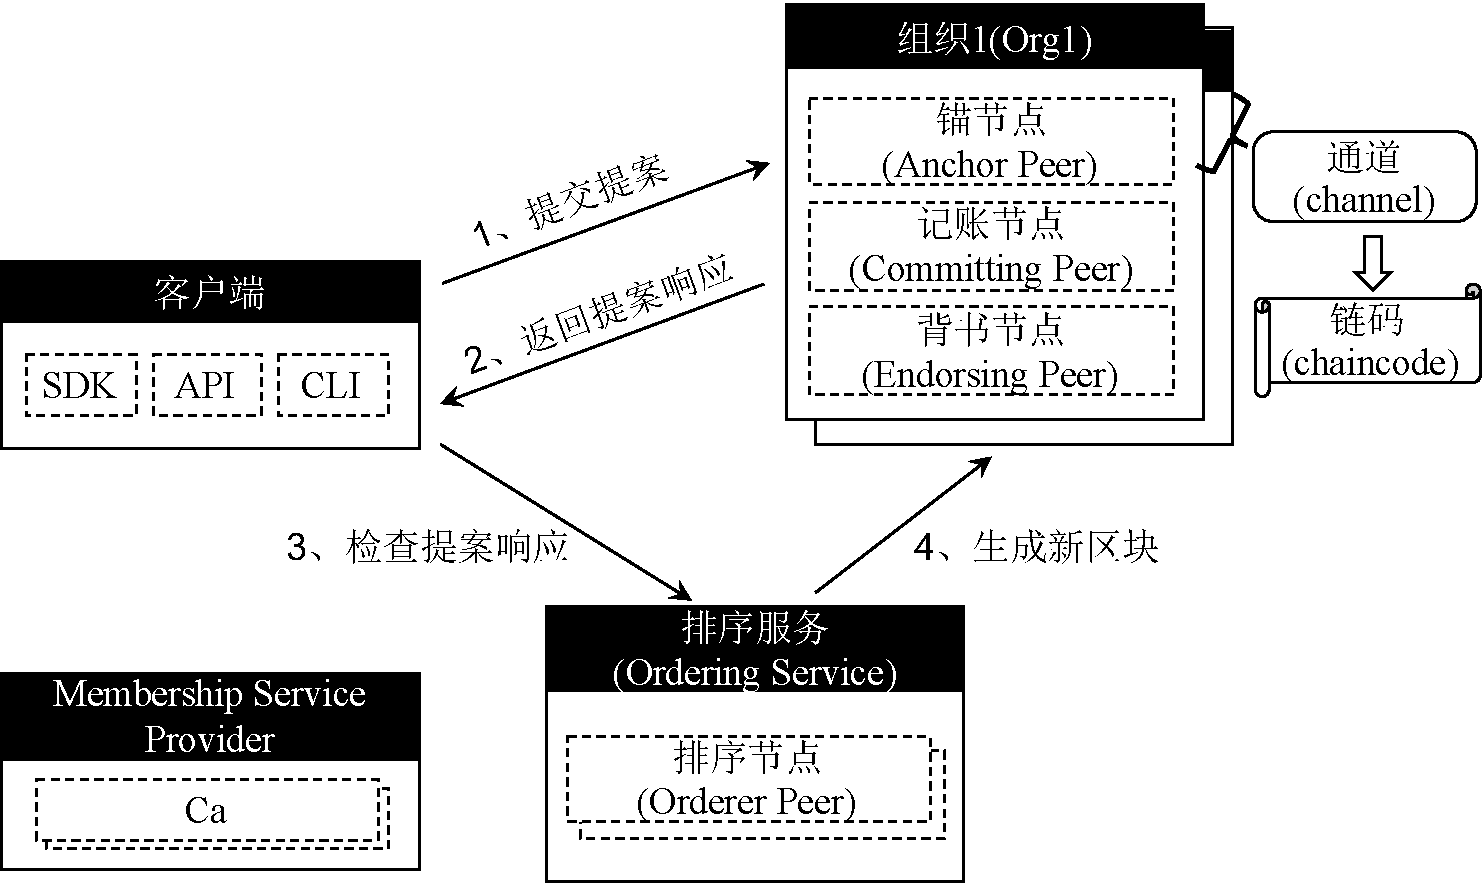
\includegraphics[width=1\textwidth]{FIGs/chapter2/hyperledger_fabric.pdf} %中括号中的参数是设置图片充满文档的大小,你也可以使用小数来缩小图片的尺寸。
    \caption{Hyperledger Fabric网络架构} %caption是用来给图片加上图题的
    \label{hyperledger_fabric} %这是添加标签,方便在文章中引用图片。
\end{figure}%figure环境 

如图\ref{hyperledger_fabric}所示, HF网络通过组织划分, 每个组织内包含多种不同角色的Peer节点, 每个Peer节点又可以担任多种角色, 所有的组织共用排序服务。HF多种节点通过网络相互链接组成联盟链网络完成链上交易。

\textbf{网络节点}
\begin{enumerate}[fullwidth,itemindent=2em,label=(\arabic*)]
    \item 客户端节点: 在HF网络外部用于主动与区块链交互、实现区块链操作的组件。常见的包含软件开发工具包(Software Development Kit, 简称SDK)\footnotemark[2]\footnotetext[2]{\href{https://github.com/hyperledger/fabric-sdk-go}{Hyperledger Fabric Go版本的SDK}}、Fabric-CLI\footnotemark[3]\footnotetext[3]{\href{https://github.com/hyperledger/fabric-cli}{fabric cli}}、REST API\footnotemark[4]\footnotetext[4]{\href{https://github.com/hyperledger/fabric/blob/v0.6/docs/source/API/CoreAPI.rst}{fabric api}};

    \item Ca节点: Fabric-Ca\footnotemark[5]\footnotetext[5]{\href{https://github.com/hyperledger/fabric-ca}{fabric ca}}是一个官方可选的Membership Service Provider组件, 对HF网络中各实体(Identity)的数字身份证书进行管理。完成实体身份注册、数字证书的签发续签或吊销;

    \item Peer节点: HF网络的每个组织都包含一个或多个Peer节点, 每个Peer节点可以通过配置文件担任一种或同时担任多种角色。

    \begin{itemize}[itemindent=2em]
        \item 锚节点(Anchor Peer): 负责与其他组织的锚节点进行通信;

        \item 记账/提交节点(Committing Peer): 负责对区块及区块交易进行验证, 验证通过后将区块写入账本中, 同时提交节点会定期与其他节点通过Gossip协议进行信息交换;

        \item 背书节点(Endorsing Peer): 负责对客户端发送的提案进行签名背书。背书节点与具体的链码(Chaincode)绑定, 其通过调用链码模拟执行交易并向生成提案的客户端返回提案响应。背书节点是动态的, 在客户端发起提案时才会根据背书策略(Endorsement policy)成为背书节点, 其他时候为记账节点。
    \end{itemize}

    \item Orderer节点: 排序服务节点接收经过背书签名的交易并对未打包的交易进行排序生成新区块, 最终通过原子广播到记账节点。排序服务采取支持可插拔设计, 支持Solo、Kafka等分布式共识协议。

\end{enumerate}

HF区块链支持在通信节点之间启用传输层安全性协议(Transport Layer Security, 简称TLS)保证两通信节点的数据保密性和完整性。TLS采用X.509证书进行身份验证并生成会话密钥, 不仅支持客户端节点对服务节点的身份验证, 同时也可以支持服务节点来验证客户端的身份的双向验证。

\textbf{账本结构}

HF中智能合约被称为链码, 通过通道(Channel)允许参与者同时履行不同的链码。HF网络子链通常按照“1个通道+1个账本+N个成员”组成。不同组织及其成员能够在通道中完成特定的交易, 限制信息传播范围。建立一个通道就相当于创建了一条子链, 这条子链上只拥有唯一的一份账本。

\begin{figure}[h] %figure环境,h默认参数是可以浮动,不是固定在当前位置。如果要不浮动,你就可以使用大写float宏包的H参数,固定图片在当前位置,禁止浮动。
    \centering %使图片居中显示
    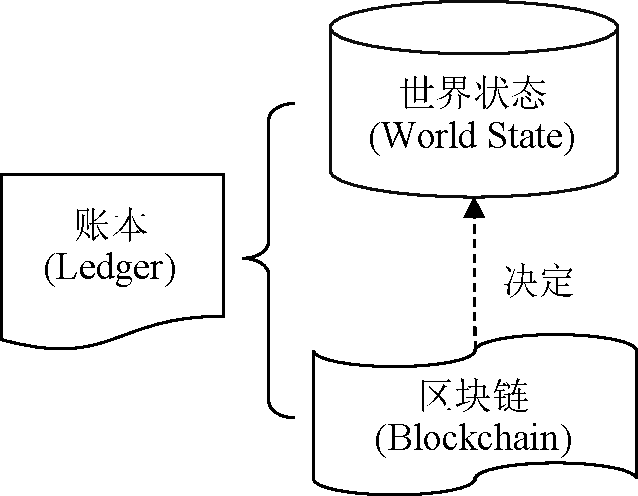
\includegraphics[width=0.45\textwidth]{FIGs/chapter2/ledger.pdf} %中括号中的参数是设置图片充满文档的大小,你也可以使用小数来缩小图片的尺寸。
    \caption{Hyperledger Fabric账本结构} %caption是用来给图片加上图题的
    \label{fabric_ledger} %这是添加标签,方便在文章中引用图片。
\end{figure}%figure环境

如图\ref{fabric_ledger}所示, HF账本由区块链以及世界状态(World State)组成, 其中世界状态由区块链决定。
首先, 世界状态是一个可插拔的键值对(key-value, 简称k-v)数据库, 提供简单、快速、丰富的账本状态检索和存储方式。通过世界状态, 客户端能够直接定位访问账本状态的某个值, 不需要遍历计算整个交易日志。为解决不同类型的问题, HF提供了LevelDB和CouchDB来保障账本状态类型的灵活性。当账本状态是简单的键值对时, 使用LevelDB合适; 当账本状态结构为 JSON时, 使用CouchDB合适。
其次, 这里的区块链指的是交易日志, 是指区块形成的链。区块记录了世界状态改变的历史, 并以文件的方式进行持久化。交易数据一旦写入区块链就无法篡改。

\subsection{Blockchain as a Service}\label{section: BaaS}

\begin{figure}[h] %figure环境,h默认参数是可以浮动,不是固定在当前位置。如果要不浮动,你就可以使用大写float宏包的H参数,固定图片在当前位置,禁止浮动。
    \centering %使图片居中显示
    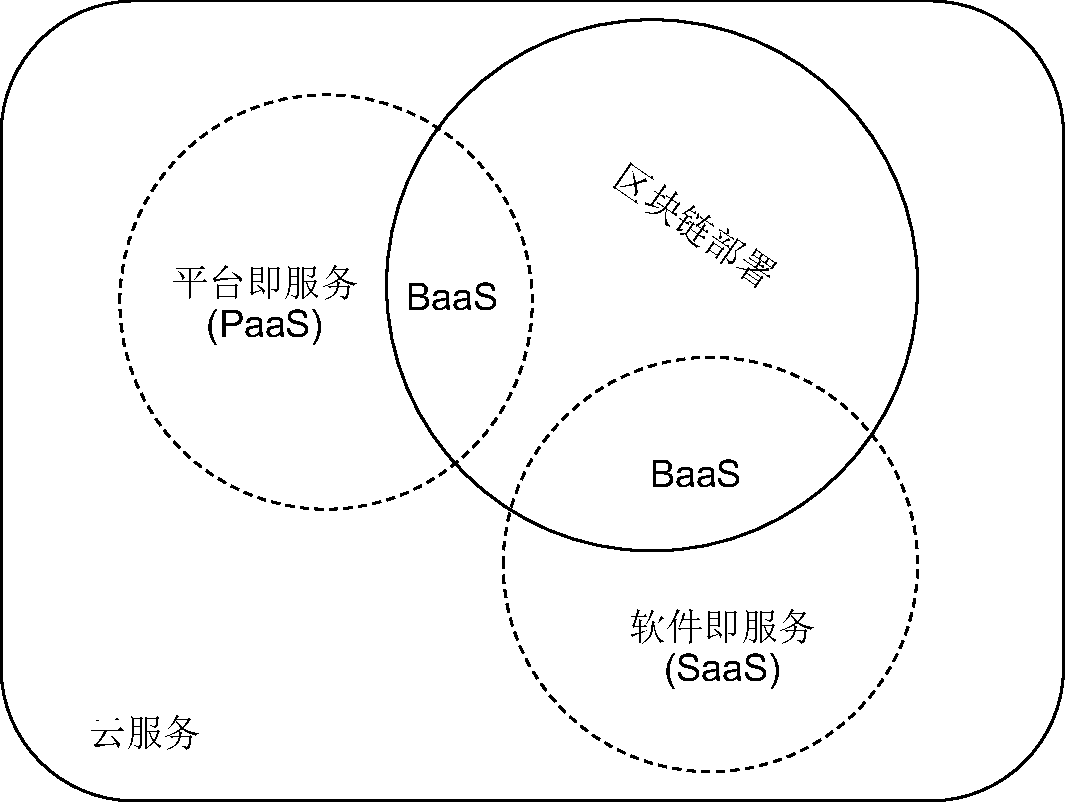
\includegraphics[width=0.55\textwidth]{FIGs/chapter2/BaaS_PaaS_SaaS.pdf} %中括号中的参数是设置图片充满文档的大小,你也可以使用小数来缩小图片的尺寸。
    \caption{BaaS与PaaS以及SaaS的对比} %caption是用来给图片加上图题的
    \label{BaaS_PaaS_SaaS} %这是添加标签,方便在文章中引用图片。
\end{figure}%figure环境

随着区块链以及云原生的发展, BaaS也悄然兴起。云提供了一种抽象、汇集和共享整个网络中的按需的、虚拟的、资源可伸缩的IT环境, BaaS则提供了一种基于云的区块链服务。BaaS能够在云上构建、管理、托管和运维区块链技术, 能够快速部署区块链网络及其开发环境、编写智能合约、构建去中心化应用(即区块链应用, Decentralized application, 简称 Dapp)。基于云基础设施, BaaS屏蔽了底层区块链与云原生的逻辑, 消除了用户构建开发去中心化应用的壁垒, 尤其是部署区块链网络所需的大量硬件和专业知识的前期成本, 为用户提供便捷的、一体化的区块链的能力。如图\ref{BaaS_PaaS_SaaS}所示, 根据BaaS的实施方式, BaaS在云环境中的位置会有所不同\cite{onik2019performance}。BaaS可以从使用平台即服务(Platform as a Service, 简称PaaS)获得基础设施支持的同时也可以通过软件即服务(Software as a Service, SaaS)获得软件服务。

微软推出由Azure云驱动的开放式区块链平台Bletchley, 该项目保证服务对于所有平台、合作者和客户来讲都是开放的、灵活的\cite{BlockchainasaServiceNextGenerationofCloudServices}。IBM推出了名为Bluemix的云计算平台, 依托于PaaS云帮助开发者更快的进行应用开发和部署。随后AWS、Google、阿里云等也相继推出自家的区块链即服务平台。以HF为例, BaaS平台通用的架构如\ref{BaaS_Architecture}所示, 本质上BaaS以计算、存储等资源为基础, 联合上层的区块链基础设施的相关能力, 如共识能力、记账能力、智能合约等转化为可编程接口, 使得区块链网络的部署以及去中心化应用开发过程简单而高效。同时, BaaS通过底层标准化的云基础设施能力为上层的区块链及其去中心化应用提供安全可靠的支撑, 解决弹性、网络、安全性、性能等难题。本文重点关注于基础设施层中Kubernetes上的区块链云化框架的研究。

\begin{figure}[h] %figure环境,h默认参数是可以浮动,不是固定在当前位置。如果要不浮动,你就可以使用大写float宏包的H参数,固定图片在当前位置,禁止浮动。
    \centering %使图片居中显示
    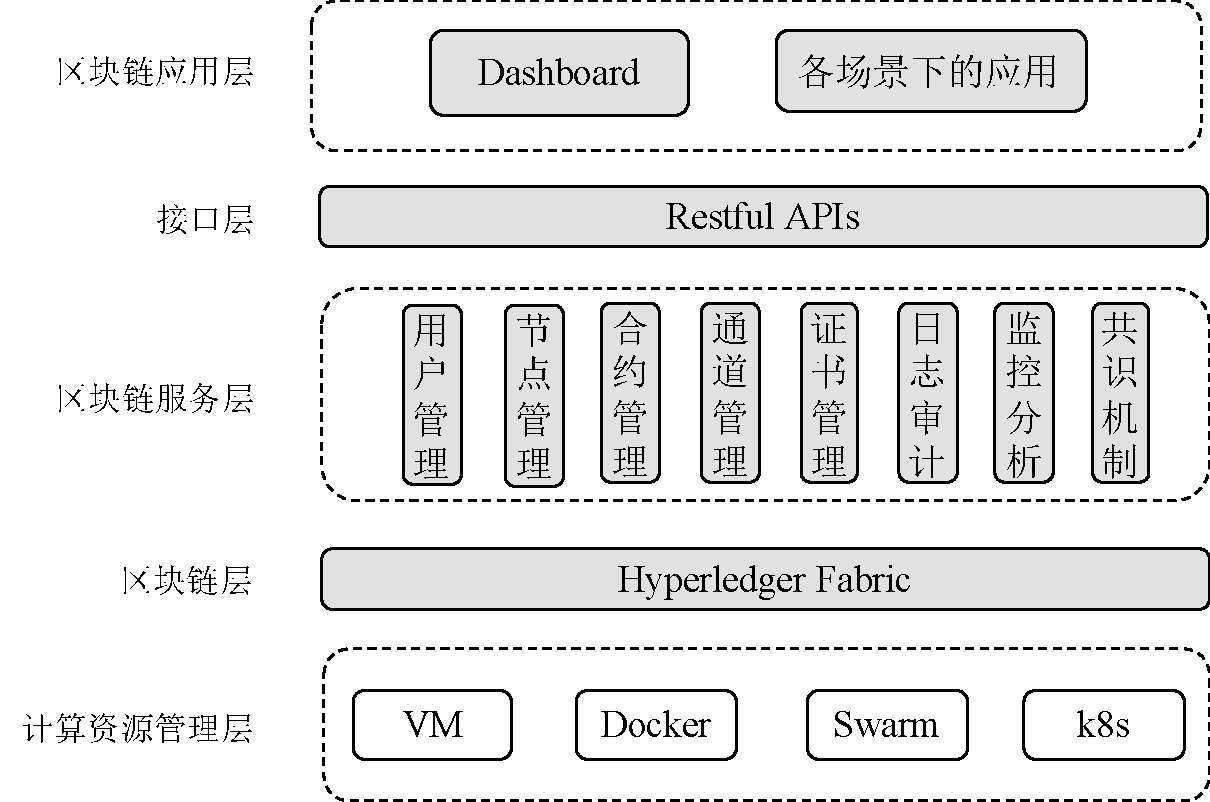
\includegraphics[width=0.85\textwidth]{FIGs/chapter2/BaaS_Architecture.pdf} %中括号中的参数是设置图片充满文档的大小,你也可以使用小数来缩小图片的尺寸。
    \caption{BaaS通用架构} %caption是用来给图片加上图题的
    \label{BaaS_Architecture} %这是添加标签,方便在文章中引用图片。
\end{figure}%figure环境

\section{云原生}\label{section: cloud_native}

\subsection{云原生基本概念}

云原生, 即云原生计算。从发展历程来说, 云原生是云计算的升级。云计算最早由Dell公司在1996年提出\cite{ZHANG20121791}, 亚马逊公司在2006年率先推出的弹性计算云(Elastic Compute Cloud, 简称EC2)服务对云计算产生了深刻影响, 越来越多的企业开始逐步接受云计算这一概念, 并将应用逐步迁移到云端, 享受这一新型计算方式带来的技术红利。此后, 软件系统规模、软件开发方式驱动着技术不断升级。在云计算的时代, 云端只是用于计算的场所, 应用无须重新编写, 只需重新部署, 应用的迁移从物理机到虚拟机, 存储选用兼容的块存储或文件存储。但几乎所有分布式场景中都需应用自行解决稳定性、数据同步、容灾等方面的问题。要解决这些问题, 只能从根本上寻求解决方案。即从迁移到云转变为诞生于云。2013年Docker开源, 之后Pivotal公司提出了云原生的概念, 这是对云计算概念的全面升级。Pivotal指出云原生由容器、微服务、DevOps以及持续交付等技术\cite{WhatisCloudNative}组成, 并充分利用云计算优势构建和运行应用。2014年, 容器编排技术Kubernetes发布。容器技术日趋成熟,在业界开始广泛应用。在2015年, 
云原生计算基金会(Cloud Native Computing Foundation, 简称CNCF)成立。而到了2021年, CNCF已经孵化了超过120个项目、740名成员以及142000的贡献者\footnotemark[1]\footnotetext[1]{\href{https://www.cncf.io/wp-content/uploads/2022/01/CNCF_Annual_Report_2021.pdf}{CNCF2021年年度报告}}。除了工业界, 云原生在学术界也引起了关注, 《计算机学报》发起了以“云原生”为主题的专刊征文\footnotemark[2]\footnotetext[2]{\href{http://chinasoft.ccf.org.cn/papers/7.html}{《计算机学报》云原生软件技术与工程实践专刊征文通知-CCF2021中国软件大会}}。

\begin{figure}[h] %figure环境,h默认参数是可以浮动,不是固定在当前位置。如果要不浮动,你就可以使用大写float宏包的H参数,固定图片在当前位置,禁止浮动。
    \centering %使图片居中显示
    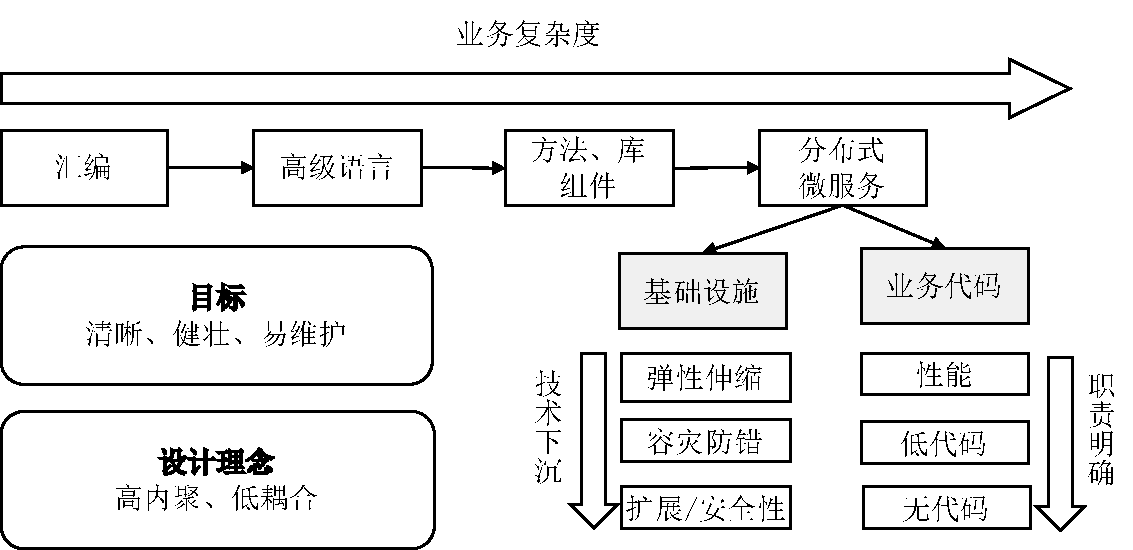
\includegraphics[width=0.9 \textwidth]{FIGs/chapter2/cloud_native_development.pdf} %中括号中的参数是设置图片充满文档的大小,你也可以使用小数来缩小图片的尺寸。
    \caption{云原生技术发展趋势} %caption是用来给图片加上图题的
    \label{cloud_native_development} %这是添加标签,方便在文章中引用图片。
\end{figure}%figure环境

以软件工程的视角来看, 如图\ref{cloud_native_development}所示, 随着软件规模、软件复杂程度在不断增大, 软件上线速度不断加快, 软件稳定性的要求在不断提高。围绕着“高内聚、低耦合”的设计理念, 软件制品进一步深层次抽象, 从单体架构演化为分布式微服务架构, 从可复用的方法、库、组件进一步下沉到底层的基础设施。在这些客观需求的驱动下, 敏捷进一步向运维端延伸, 继瀑布开发、敏捷开发之后, 开发运维一体化(Development and Operations, 简称DevOps)成为又一新兴的软件开发理念和愿景。由于软件体量巨大, 多个不同职责明确的团队负责整体软件项目的运行。DevOps旨在通过一系列文化及技术手段(尤其是自动化IT工具链)打破开发和运维团队之间的壁垒, 改善团队之间的协作关系, 实现更加频繁快速、可靠的软件产品交付\cite{ChinaDevops}。DevOps不仅将敏捷向扩展到运维端, 其更涉及到软件全生命周期中的人、流程与平台。可以说, DevOps是当下软件工程的第一生产力, 其是一种普世的价值观。云原生作为一种基于云基础设施的技术体系涵盖了云应用定义、开发、构建与运行时的所涉及到的各工具或平台。云原生是DevOps生产力下的现阶段生产工具的体现, 是DevOps 的价值具象, “DevOps 时代下的云原生”就如“蒸汽时代的蒸汽机”。

\begin{figure}[h] %figure环境,h默认参数是可以浮动,不是固定在当前位置。如果要不浮动,你就可以使用大写float宏包的H参数,固定图片在当前位置,禁止浮动。
    \centering %使图片居中显示
    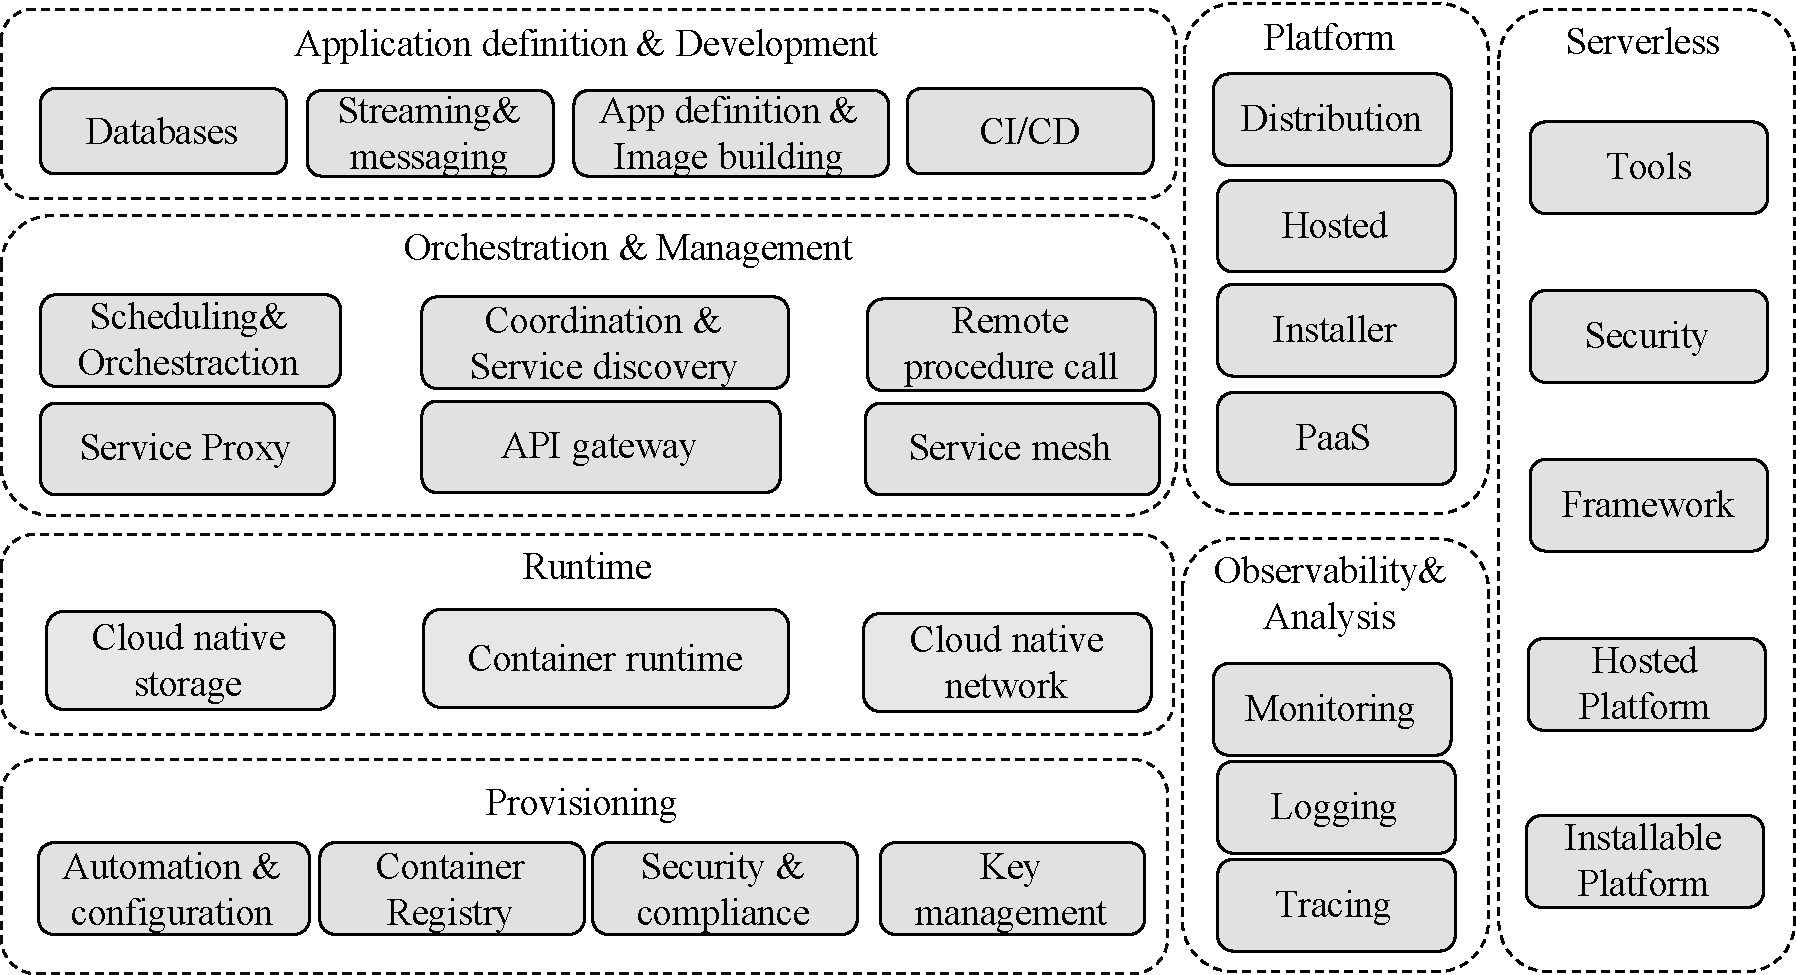
\includegraphics[width=1.0 \textwidth]{FIGs/chapter2/cloud_native_landscape.pdf} %中括号中的参数是设置图片充满文档的大小,你也可以使用小数来缩小图片的尺寸。
    \caption{云原生技术范畴} %caption是用来给图片加上图题的
    \label{cloud_native_landscape} %这是添加标签,方便在文章中引用图片。
\end{figure}%figure环境

云原生技术囊括了DevOps的各环节。如图\ref{cloud_native_landscape}所示, CNCF定义了云原生的技术范畴, 主要包括: 

\begin{itemize}[itemindent=2em]
    \item 供应层(Provisioning): 涉及云原生应用运行环境的自动化基础设施;

    \item 运行时(Runtime): 指保障云原生应用程序正常运行所需的沙盒;

    \item 云应用编排与管理(Orchestration and Management): 为云原生应用提供自动化编排和弹性伸缩能力, 让云原生应用天然地具备可扩展性;

    \item 云应用定义与开发(Application definition and Development): 开发、构建、部署和运行应用程序的工具;

    \item 可观测性与分析(Observability and analysis): 全方位监控和分析云原生应用层的工具;

    \item 平台(Platform): 主要指Kubernetes, 将多类工具有机组合在一起解决庞大的工程问题;

    \item 无服务器(Serverless): 提供函数级别更细粒度部署的一种新的云原生计算模型。
\end{itemize}


随着云架构的不断普及,“未来的软件一定生长于云上”的理念被越来越多的人所接受。云提
供了一种面向企业应用按需进行资源分配的模型, 以一种全新的高效的方式来部署应用。云原生是一系列基于云技术体系和企业管理方法的集合, 既包含了实现应用云原生化的方法论, 也包含了落地实践的关键技术。云原生应用利用容器、服务网格、微服务、不可变基础设施和声明式API等代表性技术, 来构建容错性好、易于管理和便于观察的松耦合系统, 结合可靠的自动化手段可对系统做出频繁、可预测的重大变更, 让应用随时处于待发布状态。Gartner指出, 到2022年全球公共云服务市场预计将增长至约3546亿美元, 60\%的组织将使用外部服务提供商的云管理服务\cite{bhagavan2020achieving}。企业纷纷开始云化转型, 希望将传统应用迁移到云端。

\begin{figure}[h] %figure环境,h默认参数是可以浮动,不是固定在当前位置。如果要不浮动,你就可以使用大写float宏包的H参数,固定图片在当前位置,禁止浮动。
    \centering %使图片居中显示
    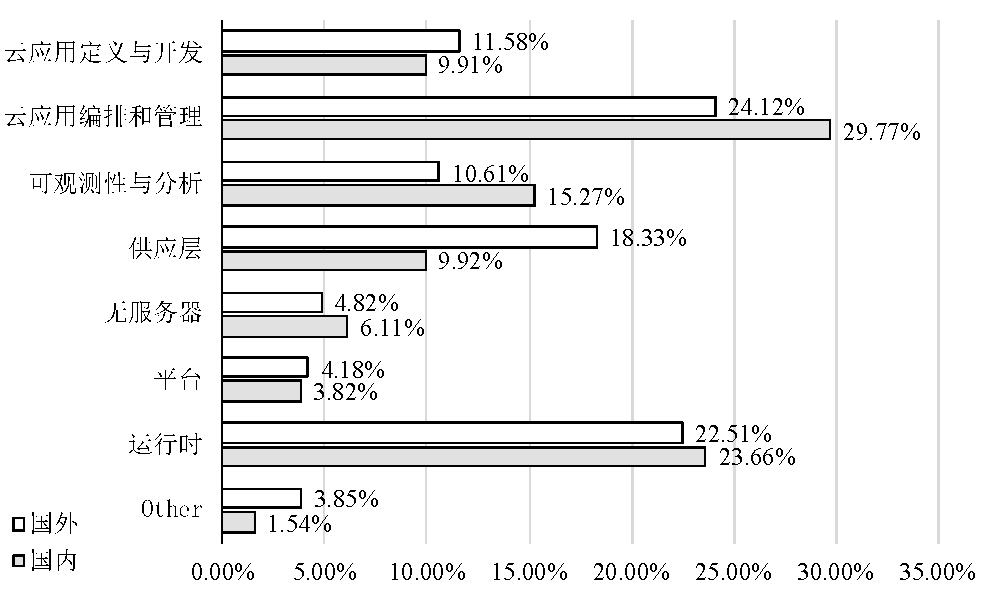
\includegraphics[width=0.9 \textwidth]{FIGs/chapter2/workshop.pdf} %中括号中的参数是设置图片充满文档的大小,你也可以使用小数来缩小图片的尺寸。
    \caption{国内外云原生技术现状} %caption是用来给图片加上图题的
    \label{workshop} %这是添加标签,方便在文章中引用图片。
\end{figure}%figure环境

如图\ref{workshop}所示, 本文根据上述7类云原生技术范畴, 对2020-2021年国内外重点技术会议的共442场分享进行了系统化分析, 其中包括国内云原生社区MeeUp城市站以及Cloud Native+Open Source Virtual Summit China共131场分享, 国际(欧洲、北美)KubeCon+CloudNativeCon Europe以及KubeCon+CloudNativeCon North America 共311篇场分享。从表中可知, 目前国内外研究重点关注于云应用编排以及运行时, 国内对云应用编排与管理的讨论要大于国际并且云应用定义与开发流程、可观测性与分析、平台与无服务器方面国内外相关分享在比例上差距并不是很大, 云原生技术体系已经成为当代软件工程技术发展的主流技术体系。

\subsection{Kubernetes}

Kubernetes(简称k8s)是Google开源的容器集群管理平台。在容器化技术之上, Kubernetes为容器化的云原生应用提供部署运行、资源调度、服务发现、弹性伸缩等一系列基础功能, 提升了大规模容器集群管理的便捷性。自开源来, Kubernetes成为一种全新的基于容器技术的分布式架构解决方案, 在云原生领域具有举足轻重的地位。2019年, 在我国72\%的工程师已经在云原生生产环境中使用大规模使用Kubernetes来进行容器\footnotemark[1]\footnotetext[1]{\href{https://www.cncf.io/blog/2020/10/13/cncf-cloud-native-survey-china-2019/}{CNCF Cloud Native Survey China 2019}}。

\begin{figure}[h] %figure环境,h默认参数是可以浮动,不是固定在当前位置。如果要不浮动,你就可以使用大写float宏包的H参数,固定图片在当前位置,禁止浮动。
    \centering %使图片居中显示
    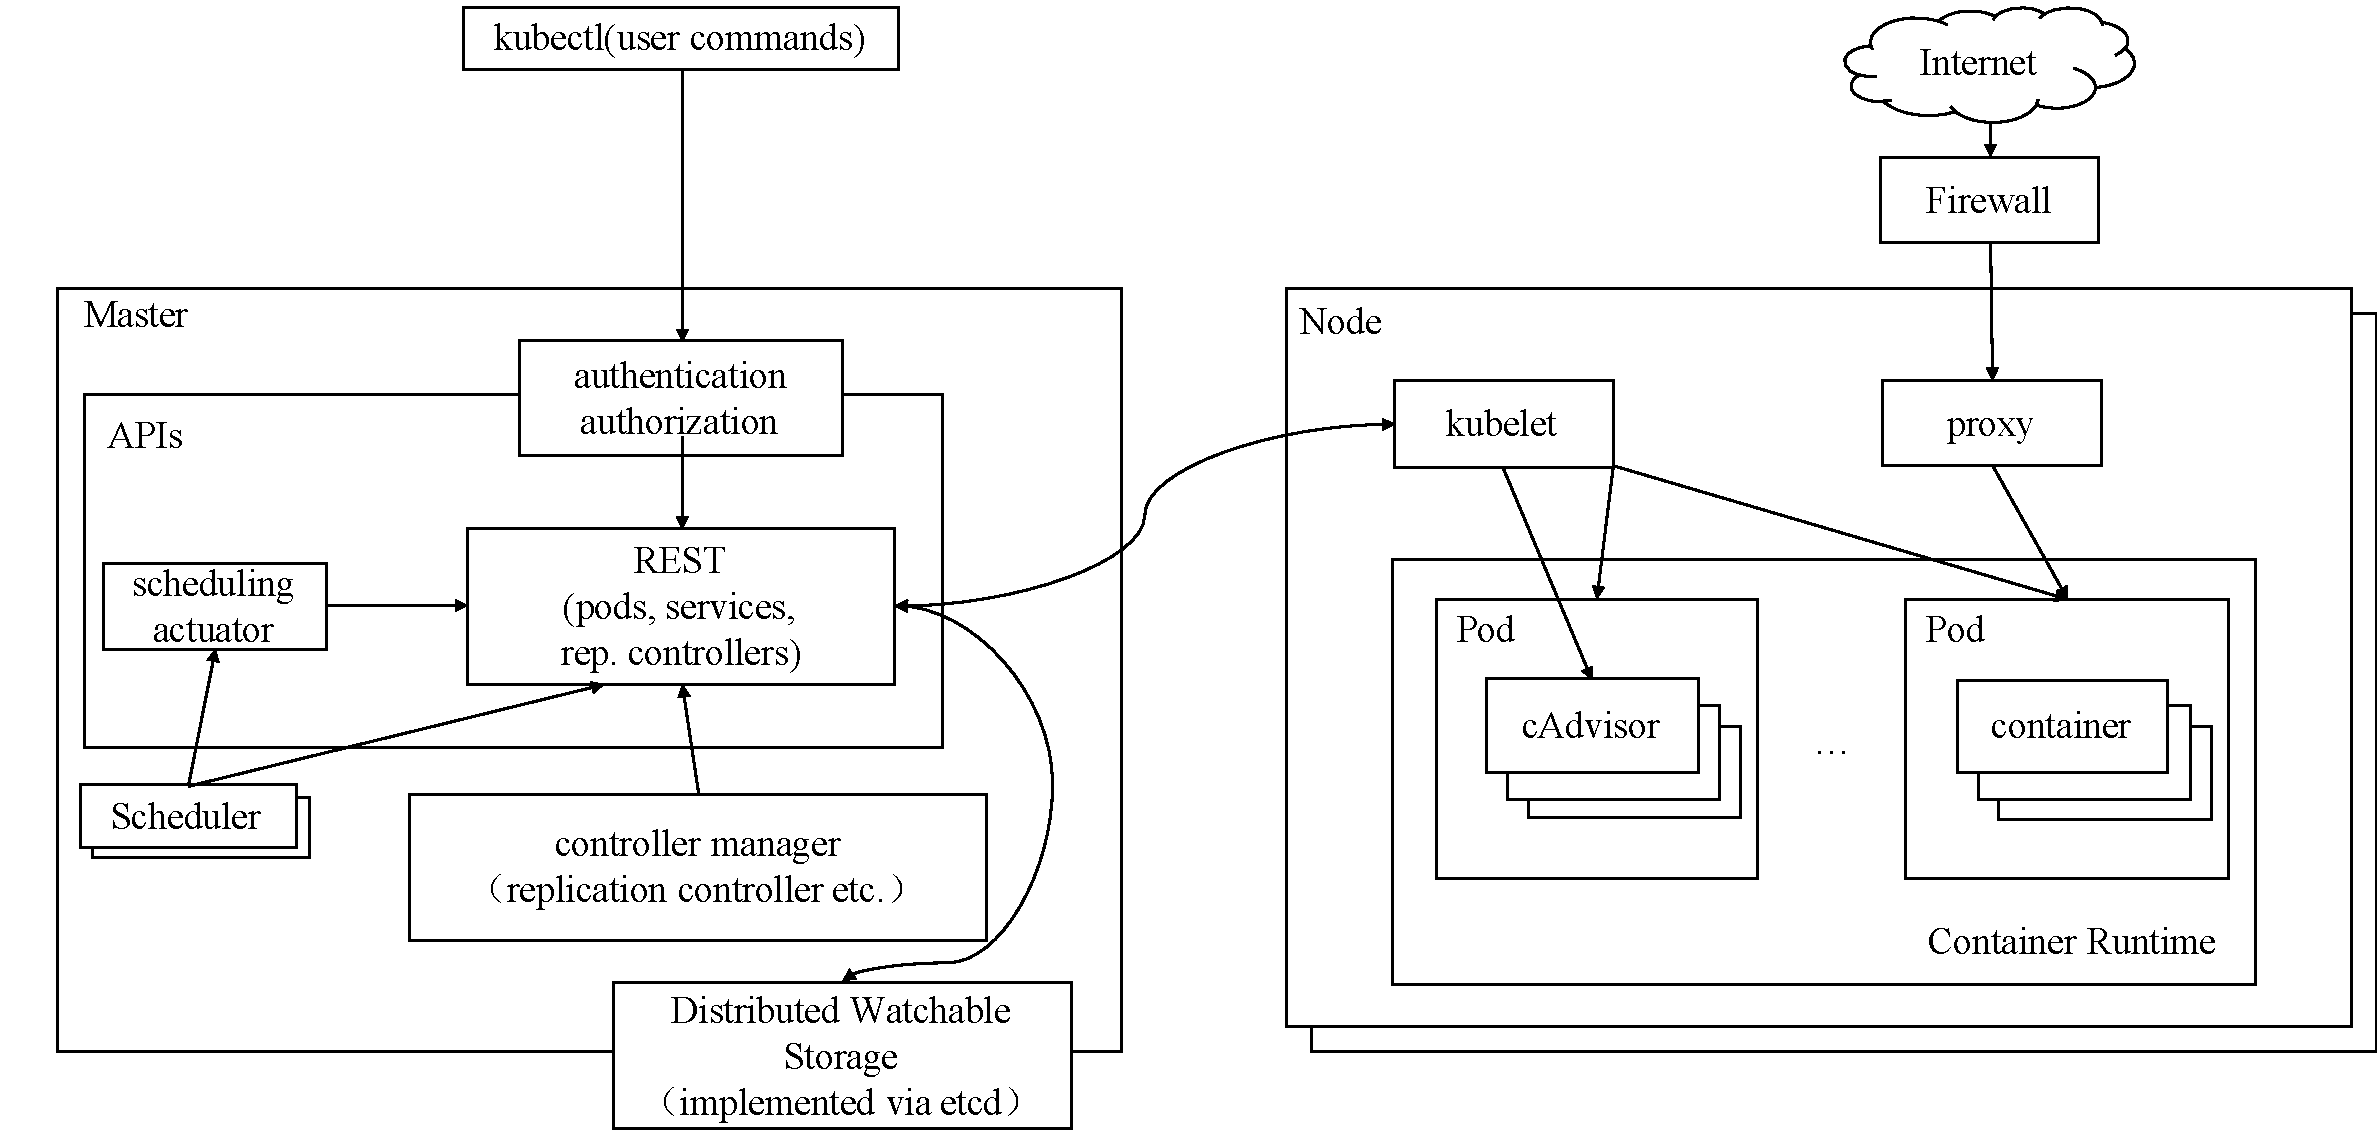
\includegraphics[width=1.0\textwidth]{FIGs/chapter2/k8s.pdf} %中括号中的参数是设置图片充满文档的大小,你也可以使用小数来缩小图片的尺寸。
    \caption{Kubernetes架构图} %caption是用来给图片加上图题的
    \label{k8s} %这是添加标签,方便在文章中引用图片。
\end{figure}%figure环境

Kubernetes由节点代理(kubelet)和Master节点组成。如图\ref{k8s}所示, Kubernetes节点主要由以下核心组件构成:

\begin{itemize}[itemindent=2em]
    \item Etcd: 用于保存集群中一切网络配置和状态信息;

    \item APIServer: 是资源配额控制的入口, 具备完备的集群安全机制并且提供用于集群管理的REST API接口;

    \item Controller Manager: 集群内部的所有资源的管理控制中心, 负责集群内的Node、Pod副本、Endpoint、Namespace、ServiceAccount、ResourceQuota的管理, 实现自动扩展、自动滚动更新、故障检测等功能;

    \item Sheduler: 根据特定的调度算法将Pod调度到指定的工作节点;

    \item kubelet: 定时检查获取节点上Pod、容器的期望状态, 并调用对应的容器平台接口达到这个状态;

    \item Container Runtime: 负责镜像管理以及Pod和容器的真正运作\cite{wangjunxiang2018};

    \item kube-proxy: 为Service提供集群内部的负载均衡和服务发现。
\end{itemize}

Kubernetes拥有独特的声明式API设计, 即声明式地告诉Kubernetes所需资源的状态, 而不是告诉它如何做。在Kubernetes中对象(Object)是持久化的实体, Kubernetes使用这些实体去表示整个集群的状态, 同时这些对象可以在Yaml\cite{ben2009yaml}文件中作为一种声明式API类型来灵活的创建并配置。典型的, Kubernetes的对象主要有以下几种: 

\begin{itemize}[itemindent=2em]
    \item Namespace: 能够隔离资源。Kubernetes集群可以拥有多个命名空间, 这些命名空间在逻辑上彼此隔离, 实现了对多用户的资源隔离;

    \item Pod: Kubernetes中最基本的操作单元, 包含一个或多个容器。Kubernetes为每个Pod分配一个唯一的IP地址, Pod内部的多个容器共享该IP地址。并且每个Pod都能设定自己的计算资源, 即CPU和Memory;

    \item Replication Controller(简称RC): 确保任意时间Kubernetes集群中运行指定数量的Pod副本;

    \item Deployment: 保证Pod的数量和健康, 绝大多数的功能与RC完全一样, 能够被当作全新一代的RC;

    \item Service: 定义了一个Pod逻辑集合以及访问Pod的策略, 它提供一种桥梁会为访问者提供一个固定的Pod访问地址用于在访问时重定向到相应的后端;

    \item Label: 通过键值对的方式被附加到任何资源对象上, 用于配置资源;

    \item Secret: 不需要将敏感数据外露, 解决密码、token、密钥等敏感数据的配置问题;

    \item Role: 一组权限的集合, 给某个NameSpace中的资源进行鉴权;

    \item ConfigMap: 为了让镜像和配置文件解耦, 应用程序会从配置文件、命令行参数或环境变量中读取配置信息,以便实现镜像的可移植性和可复用性;

    \item Volume: Pod中能够被多个容器访问的持久化共享目录;

    \item Persistent Volume(简称PV): 类似于Volume, Kubernetes提供的存储资源的抽象管理集群存储, 其API内包含存储的细节实现;

    \item Persistent Volume Claim(简称PVC): 对存储资源的请求声明, PVC不关心底层存储实现的细节, 只消耗PV资源。

\end{itemize}

随着Kubernetes生态的持续发展, 上述常规的资源类型仅代表通用的对象, 并不能适应多变的业务需求。为提升自身的扩展能力, Kubernetes提供用户自定义CRD向Kubernetes API中增加定制化的资源类型。用户的自定义资源(Custom Resource, 简称CR)创建并注册到Kubernetes API后, 其与常规通用资源对象都是原生的、存在于etcd中的同等资源, 可以采用Kubernetes原生方式进行创建、查看。CRD本质上用于声明用户自定义资源对象, 开发人员还需要针对CRD提供关联的Operator对CR进行完整生命周期管控。

Operator主要负责有状态应用(即CR)及其组件的部署、更新、自动扩展、维护、数据备份等, 保证其可用性。其作为Kubernetes的一种扩展形式, 基于Kubernetes的资源和控制器(Controller)概念构建, 遵循Kubernetes原则, 功能类似于Controller Manager, 但同时又注入了特定领域知识。

\section{其他相关技术}\label{section: other_technologies}

\subsection{Helm}

Helm是一种基于Kubernetes云计算平台的打包和部署复杂软件应用程序的技术\cite{spillner2019quality}。随着云原生及微服务架构的发展, 开发人员倾向于将大的单体应用分解成多个可以独立开发、部署、运维的微服务部署于Kubernetes之上。服务数量的增加为Kubernetes编排带来了复杂性, Helm则通过软件打包的方式极大的简化了Kubernetes应用部署和管理的复杂性。

Helm存在三个核心概念:

\begin{itemize}[itemindent=2em]
    \item chart: 即一系列包含创建Kubernetes应用实例必要信息的文件;

    \item config: 包含应用发布的相关配置信息;

    \item release: chart及其配置的运行实例。
\end{itemize}

如图\ref{helm}所示, Helm将Kubernetes资源(如Deployment、Service)打包到chart中, chart将会被保存到仓库中。Tiller是部署于Kubernetes中的Helm的服务端, 负责接受Helm请求并于APIServer进行交互, 根据chart生成并管理release。开发者使用Helm可以简化应用配置及版本管理, 使得在Kubernetes上部署、升级、回滚、卸载应用程序更加方便。

\begin{figure}[h] %figure环境,h默认参数是可以浮动,不是固定在当前位置。如果要不浮动,你就可以使用大写float宏包的H参数,固定图片在当前位置,禁止浮动。
    \centering %使图片居中显示
    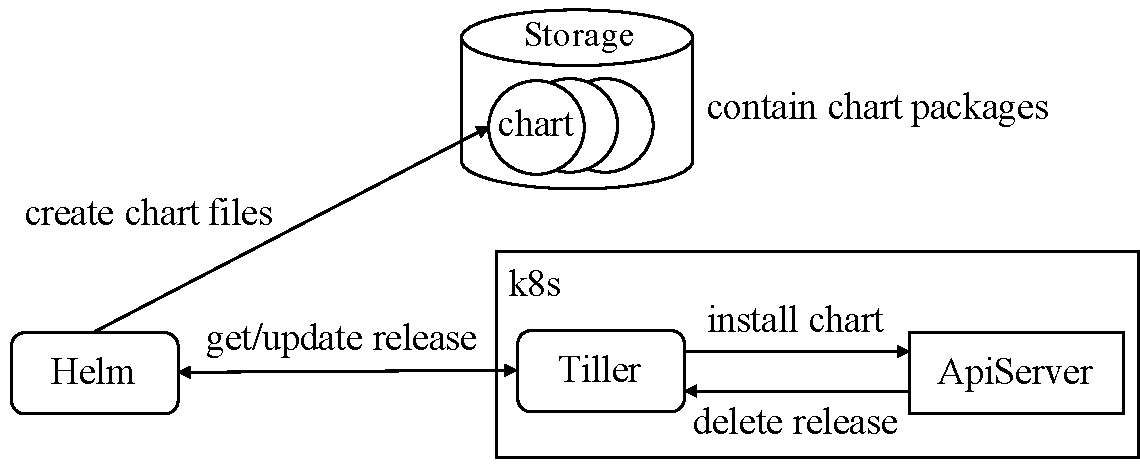
\includegraphics[width=0.8\textwidth]{FIGs/chapter2/helm.pdf} %中括号中的参数是设置图片充满文档的大小,你也可以使用小数来缩小图片的尺寸。
    \caption{Helm架构图} %caption是用来给图片加上图题的
    \label{helm} %这是添加标签,方便在文章中引用图片。
\end{figure}%figure环境

% \subsection{Istio}

% 随着技术下沉, 传统由软件本身负责的负载均衡、路由等功能下沉到云原生基础设施。服务网格(Service Mesh)通过在不断变化的条件和拓扑结构面前强制执行所需的网络行为, 为网络连接的工作负载提供基于策略的网络服务\cite{calcote2019istio}。Istio\footnotemark[1]\footnotetext[1]{\href{https://github.com/istio/istio}{istio}}是Service Mesh架构的一种实现方式, 其是一个用于保证容器服务间连接、安全、控制和观测的网络代理组件, 具有负载均衡、服务间认证、监控等功能。

% Istio分为两个逻辑部分\cite{larsson2020impact}: 数据平面(Data Plane)与控制平面(Control Plane)。数据平面由代理程序Envoy(通常被称为Sidercar)组成, 其受控制平面组件控制, 通常与业务容器捆绑, 来劫持业务应用容器的流量完成针对特性应用程序的控制与治理; 控制平面提供服务发现、配置和证书管理等功能, Istio对其进行了进一步细分:

% \begin{itemize}[itemindent=2em]
%     \item Mixer: 负责策略、访问控制和请求追踪;

%     \item Pilot: 提供服务发现的功能;

%     \item Citadel: 负责证书颁发;
% \end{itemize}

\section{本章小结}

本章\ref{section: blockchain}节首先介绍了区块链基本概念、架构、分类, 其次重点介绍联盟链解决方案HF的网络节点、账本结构, 最后介绍区块链即服务的诞生和通用架构; \ref{section: cloud_native}节介绍云原生的发展历程、技术范畴以及Kubernetes; \ref{section: other_technologies}节介绍本文区块链云化架构涉及到的其他相关技术。

% \begin{figure}[!htbp] %figure环境,h默认参数是可以浮动,不是固定在当前位置。如果要不浮动,你就可以使用大写float宏包的H参数,固定图片在当前位置,禁止浮动。
%     \centering %使图片居中显示
%     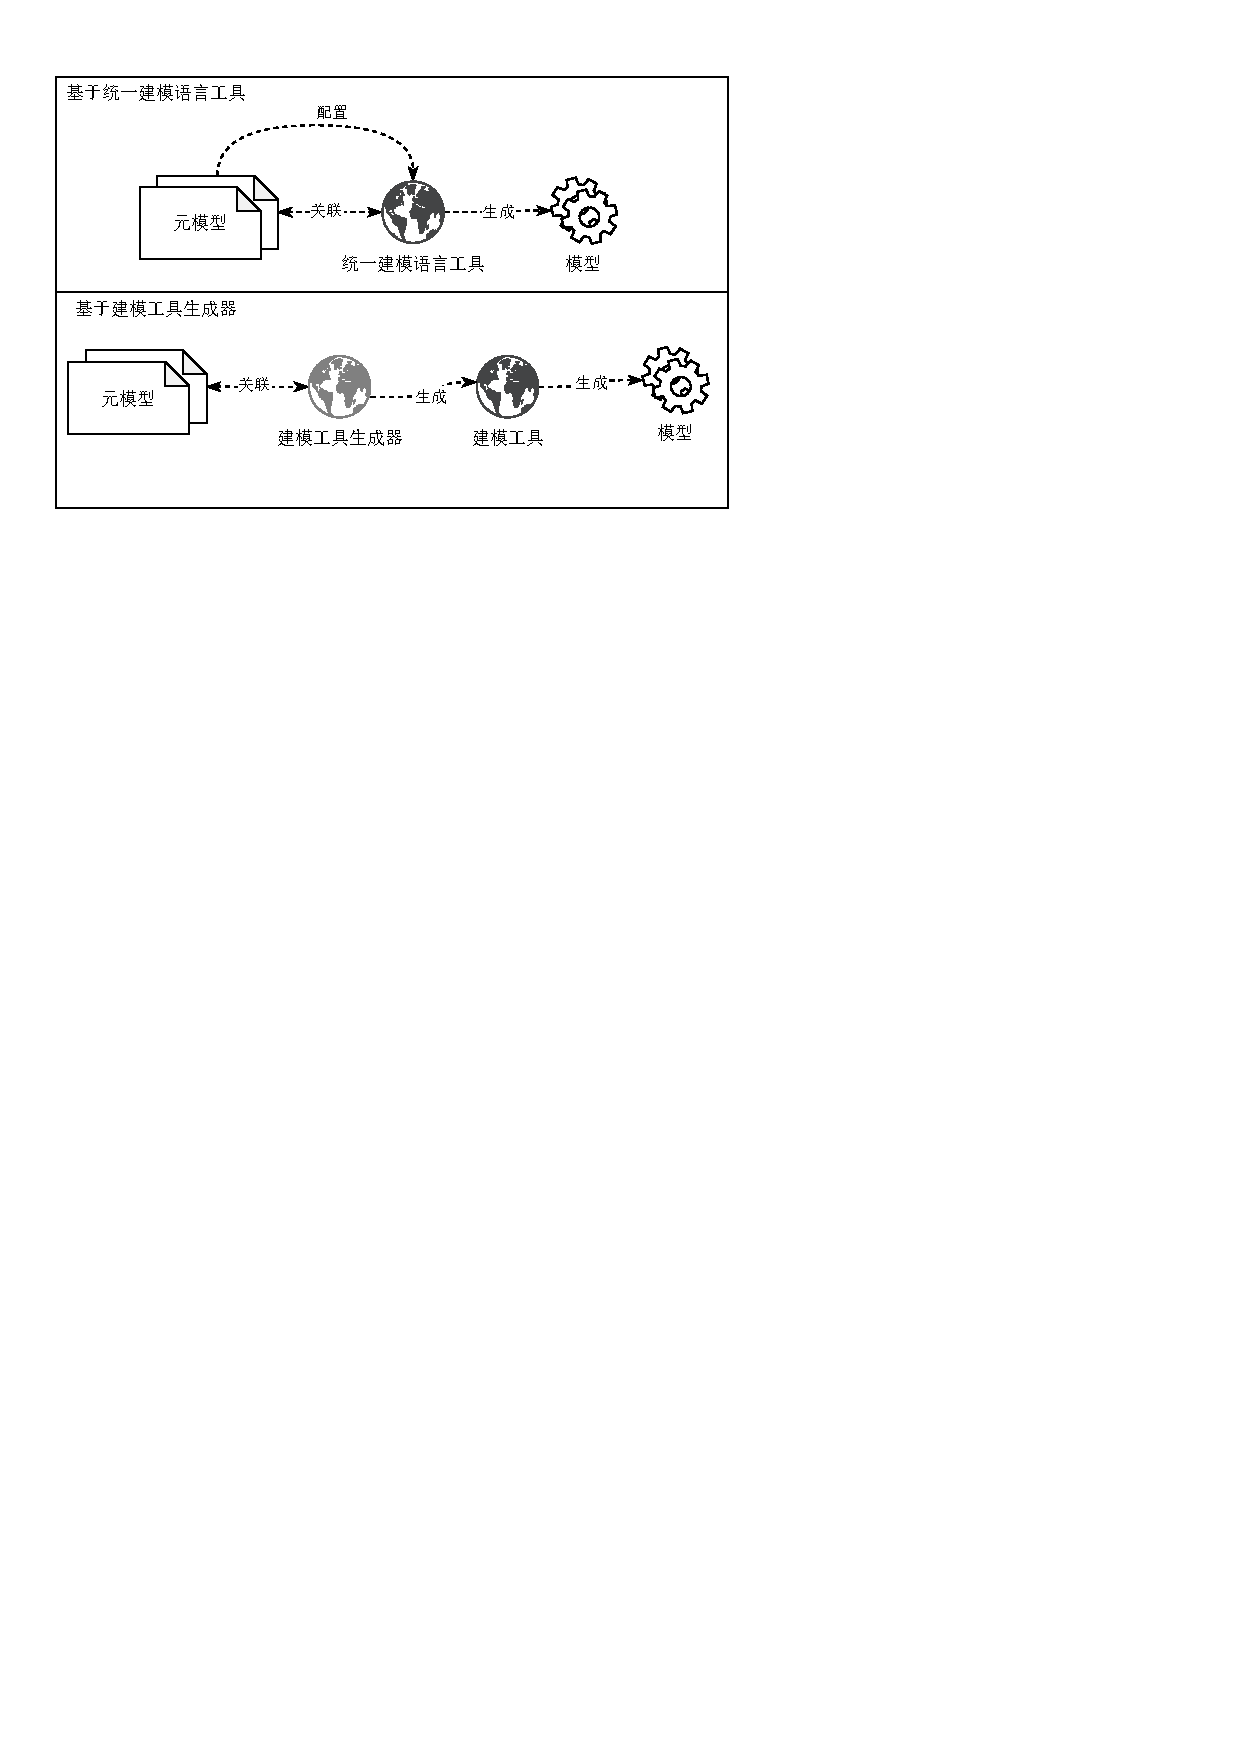
\includegraphics[width=0.8\textwidth]{FIGs/chapter3/2kindsmodeling.pdf} %中括号中的参数是设置图片充满文档的大小,你也可以使用小数来缩小图片的尺寸。
%     \caption{两种建模工具实施方式} %caption是用来给图片加上图题的
%     \label{2kindsmodeling} %这是添加标签,方便在文章中引用图片。
% \end{figure}%figure环境







\chapter{面向领域驱动设计的战术建模支持方法}

\section{研究方法概述}

领域驱动设计的概念已经在工业界得到运用,但在针对领域驱动设计进行建模时,
尤其是战术建模时,没有一套标准的建模语言和流程规范进行指导和约束,
导致战术建模过程难以实施,建模结果难以落地,落地后无法进行复用和扩展。
本文工作的核心目标之一是提出一套针对战术建模的支持方法,
包含战术建模指南和实例化的战术建模语言,用来支持战术建模工作。

本节将对提出战术建模支持方法的研究方法和各阶段产物进行概述,
具体内容如图\ref{researchmethod}所示。
为了构建一套包含战术模式、战术模式重要属性、使用时机以及实现技术的战术建模指南,
本文工作首先对战术建模和元模型领域进行调研,
通过文献综述收集整合领域驱动设计权威著作中的理论知识。
文献综述(Literature Review)是对某一研究领域的问题搜集大量相关资料,
通过阅读、分析、提炼、整理该领域最新进展和学术成果,
对其做出归纳性整理和综合性介绍的一种研究方式。
其次,结合从文献中收集的知识,设计访谈问题,
对工业界内战术建模的实践者进行访谈。
访谈法(Interview)是以口头形式根据受访者的回答搜集客观事实材料的
一种研究性交谈方式,通过访谈法不断迭代完善现有知识,形成最终的建模指南。
% 战术模式描述了战术建模中常用的模式,充当了业务领域概念映射到建模中的载体;
% 战术模式重要属性和战术模式使用时机描述了战术建模的特征和使用场景;
% 战术模式实现技术描述了战术建模实现层面的最佳实践,可以作为战术建模实现时的技术方案参考和指导。

以调研的初步产物为基础,结合焦点小组法(Focus Group)\cite{fattahi2018focus},构建战术建模支持方法。
焦点小组是通过召集一组与研究主题相关的人员对同一议题进行讨论,并得出深入结论的定性研究方法,
焦点小组产出的战术建模支持方法包括战术模式及属性列表、战术建模语言以及一套战术建模使用时机与实现技术指导。
本文工作对战术建模语言进行了实例化和工具支持,主要包含建模语言元模型、对象约束语言(OCL)和具体表示方法。


\begin{figure}[h] %figure环境,h默认参数是可以浮动,不是固定在当前位置。如果要不浮动,你就可以使用大写float宏包的H参数,固定图片在当前位置,禁止浮动。
    \centering %使图片居中显示
    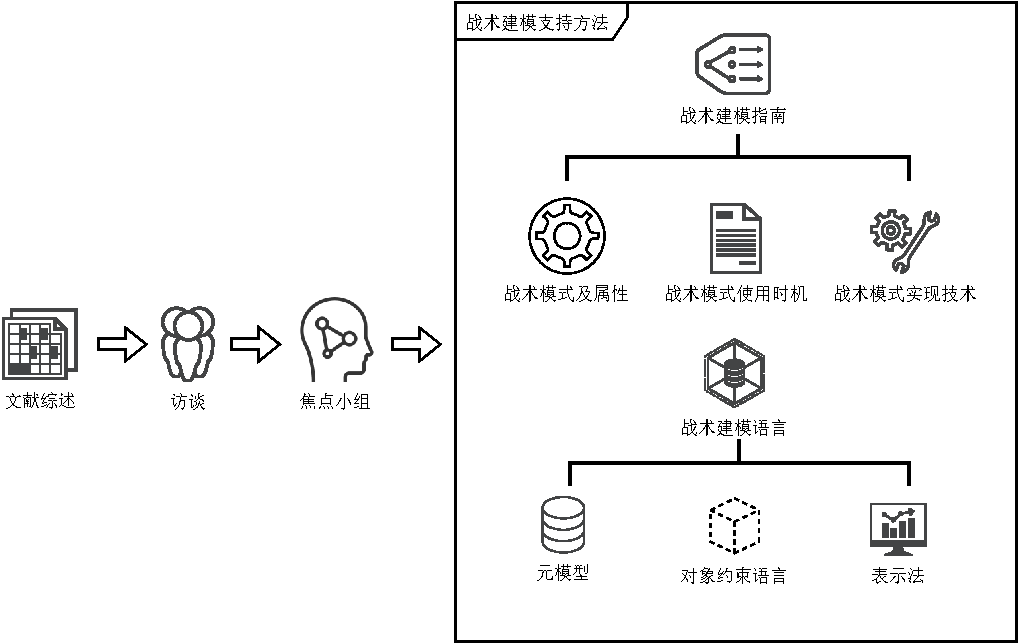
\includegraphics[width=0.8\textwidth]{FIGs/chapter3/researchmethod.pdf} %中括号中的参数是设置图片充满文档的大小,你也可以使用小数来缩小图片的尺寸。
    \caption{战术建模支持方法研究过程图} %caption是用来给图片加上图题的
    \label{researchmethod} %这是添加标签,方便在文章中引用图片。
\end{figure}%figure环境

\section{研究过程}

\subsection{文献综述}

本小节主要介绍文献综述相关工作。
文献综述总结了前人的工作成果,
从领域驱动设计相关著作中进行战术模式的收集与定义。
本工作从战术模式中抽取了重要特征,提高实例化战术建模语言的效率与正确性。
总结了战术建模的使用时机与实现技术,作为战术建模支持方法的一部分。
本工作在调研阶段还参考了相关文献中提出元模型的流程方法,作为元模型构建的理论基础,
对现有领域驱动设计建模元模型的特征进行研究和总结,吸取元模型构建经验。

作者从《领域驱动设计:软件核心复杂性应对之道》\cite{DBLP:books/daglib/0013521}、
《实现领域驱动设计》\cite{vernon2013implementing}两本著作中抽取了八种战术建模模式以及它们的
重要特征,并以此为基础,构建了一个特定于领域驱动设计战术建模的初始元模型。
Evans认为使用领域驱动设计的人员需要经常快速地浏览一些重要的模式,
并掌握这些模式的实施要点和特征,
并与实际业务进行结合使用\cite{evans2014domain}。
领域驱动设计中的概念知识,特别是更为分散的战术模式相关概念知识繁多复杂,需要在使用时经常进行学习和回顾,
确保实践的准确性,
这也是将战术模式属性、使用时机和实现技术纳入建模支持方法的一个重要原因。


在本小节总结的成果中,战术建模模式包括:实体(Entity)、值对象(Value Object)、
领域服务(Domain Service)、领域事件(Domain Event)、聚合(Aggregate)、
资源库(Repository)、模块(Module)、工厂(Factory)。
战术模式重要特征描述了战术模式应该具备的特点、约束条件以及它和不同模式间的关系。
战术模式应用场景描述了每个模式的使用时机和实现时的核心问题。
上述成果将作为访谈问卷的理论基础,经过访谈不断迭代完善,
最终形成关于战术模式的使用指南。

\subsection{访谈}

% 根据文献综述成果,设计问卷问题,
% 对3名工业界内领域驱动设计战术建模的实践者进行访谈并总结访谈结果。
通过分析多次访谈的结果,
对文献综述阶段得到的战术模式进行验证和筛选,
对战术模式重要特征、使用时机和实现技术进行确认和修改,
总结出一套战术建模指南。

访谈活动共进行三次,每次访谈一名对象,访谈持续时间控制在一小时左右。
表\ref{respondents}展示了访谈对象的具体信息,
三名访谈对象分别来自思特沃克、阿里巴巴和华为,
其中有两名架构师和一名开发人员。

{\footnotesize
\begin{longtable}[h]{m{70pt}|m{60pt}|m{255pt}}
    \caption[受访者信息]{受访者信息} \label{respondents} \\
        \hline  
        业务领域&角色&从业经验及年限\\
        \hline
        软件咨询领域&架构师&就职于斯特沃克(ThoughtWorks),
        为国内外医疗、金融、通信、汽车等行业的客户提供软件咨询和交付服务。
        作为技术顾问参与和主导了多次领域驱动设计相关工作,
        是将领域驱动事件风暴引入国内的第一批技术人员。
        拥有10年左右的开发及架构设计经验。\\
        \hline
        通信领域&架构师&就职于华为,
        使用领域驱动设计相关思想与方法多次主导并参与过大型分布式项目的架构设计与微服务拆分。
        拥有10年以上的开发及架构设计经验。\\
        \hline
        电商领域&开发人员&就职于阿里巴巴,
        担任过项目经理,参与过微服务开发,具有战术建模的实践经验,
        对领域驱动设计有过一定了解。
        拥有2年左右的开发及项目管理经验。\\
        \hline

    \end{longtable}
}

访谈首先对访谈对象的个人信息进行了解,包括受访对象的职位、团队规模以及业务领域,
方便对领域驱动设计战术建模实践场景进行评估;
然后对领域驱动设计建模过程进行了解,包括建模使用的工具,建模工作的总体流程,
用来和本文工作做对比,评估本文工作对战术建模领域的作用;
最终聚焦战术建模中的战术模式,对文献综述阶段总结的成果进行评估。
如表\ref{reviewQ}所示,展示了访谈中主要关注的五个方面,
并阐述了具体原因。
具体访谈问卷问题见附录\ref{app:1}。
在访谈中,
受访对象均对本文工作研究内容和最终产出的支持工具持积极态度。

{\footnotesize
\begin{longtable}[h]{m{170pt}|m{215pt}}
    \caption[访谈关注问题]{访谈关注问题} \label{reviewQ} \\
        \hline  
        关注问题&原因\\
        \hline
        何时使用该模式&获取和验证战术模式的使用时机。\\
        \hline
        该模式应该包含哪些重要属性&获取和验证战术模式的属性。\\
        \hline
        实践该模式时有哪些好的实践&获取和验证战术模式的实现技术与细节。\\
        \hline
        实践该模式时有哪些不好的实践&排除不好的实现技术。\\
        \hline
        针对于特定模式的特殊问题&验证对应战术模式是否有必要加入建模支持方法。\\
        \hline
    \end{longtable}
}



\subsection{焦点小组}

本小节介绍研究过程中使用焦点小组形式进行战术建模支持方法构建的相关内容。在所有访谈结束后,
组织焦点小组对文献综述与访谈结果进行分析和评估,目的是不断完善战术建模支持方法内容,
包括迭代和实例化战术建模语言,总结整合战术模式、模式属性、使用时机以及实现技术。

每次焦点小组由包含作者在内的三名研究人员参与,
作者为主持人兼记录员,
负责主持会议和记录会议内容,
其他与会人员均对领域驱动设计相关知识具有一定了解。

如图\ref{focusgroup}所示展示了焦点小组的详细实施过程。
在会议开始前,先将前期文献综述与访谈的成果作为资料展示给参与人员,
并由主持人介绍访谈的初步成果。
会议开始后,使用领域驱动设计战术建模中的重要概念以及会议资料对战术建模支持方法进行设想。
首先,将文献综述和访谈结果中的战术模式与其重要特征进行整合,形成战术模式及其属性列表;
在整合过程中,找出重复和互补的修改建议,使最终战术模式与特征列表更加准确完善,
更好地充当构建战术建模语言时的附加属性;
通过UML profile机制构建元模型,
并设计对象约束语言和建模语言表示方法来实例化战术建模语言;
最后,将战术模式使用时机与实现技术纳入到战术建模指南中;
经过多次焦点小组的讨论和修改后,
战术模式、战术模式的属性、使用时机以及实现技术共同组成了战术建模指南,
汇总战术建模指南和实例化的战术建模语言,形成最终的战术建模支持方法,并对其进行评估。


% 并从访谈结果中抽取战术模式重要特征,找出重复和互相补充的修改建议,形成汇总之后的修改结果,
% 修改后的结果包括战术模式的特征与属性、战术模式之间的关系与约束以及战术建模的实践经验;
% 对总结的结果进行评价,
% 经过多次焦点小组后,使用元模型构建方法(UML profile机制)将修改后的结果添加到元模型中,
% 使用对象约束语言等方式完善建模语言并将新的战术建模实践经验加入到框架中,
% 最终产出一套完整的战术建模框架,整个过程如图\ref{focusgroup}所示。

\begin{figure}[!htbp] %figure环境,h默认参数是可以浮动,不是固定在当前位置。如果要不浮动,你就可以使用大写float宏包的H参数,固定图片在当前位置,禁止浮动。
    \centering %使图片居中显示
    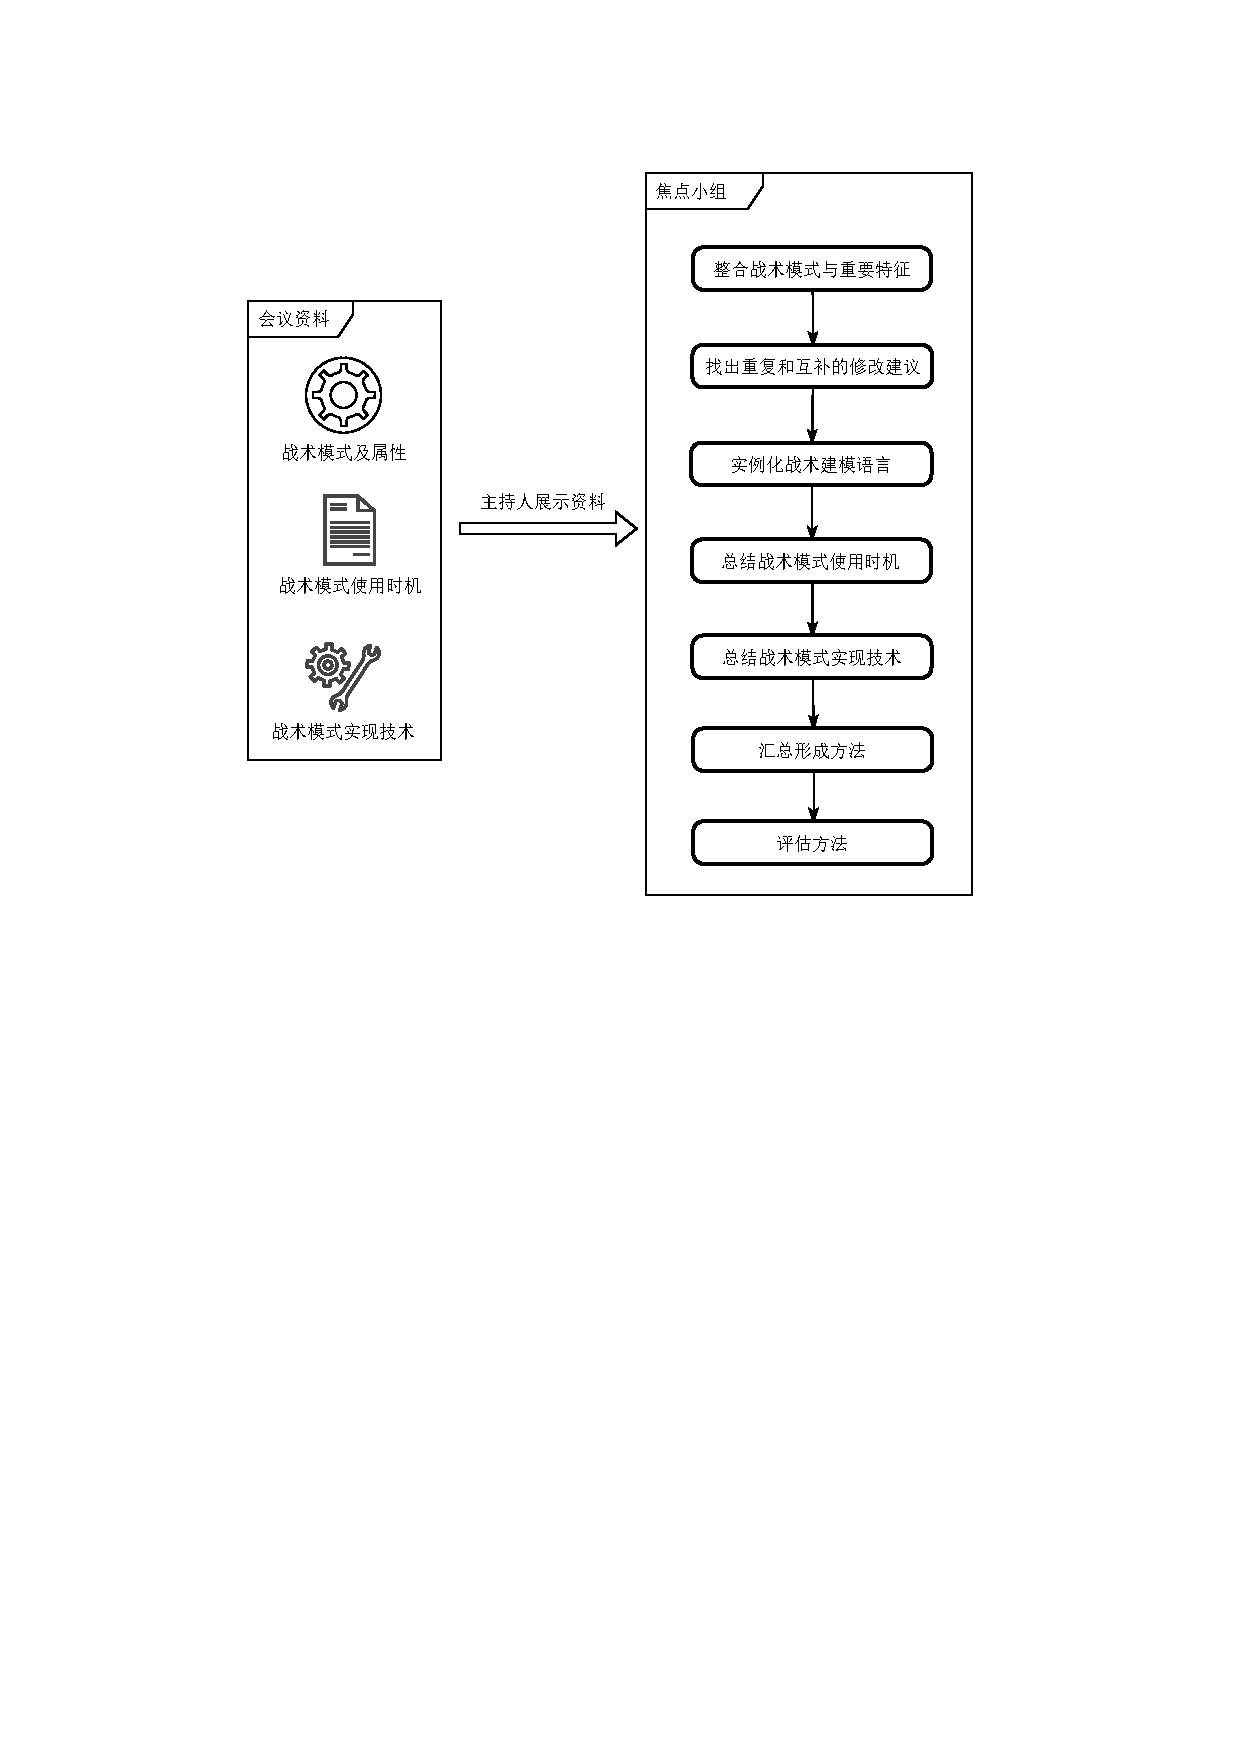
\includegraphics[width=0.8\textwidth]{FIGs/chapter3/focusgroup.pdf} %中括号中的参数是设置图片充满文档的大小,你也可以使用小数来缩小图片的尺寸。
    \caption{焦点小组实施过程} %caption是用来给图片加上图题的
    \label{focusgroup} %这是添加标签,方便在文章中引用图片。
\end{figure}%figure环境

\section{战术建模指南}

\subsection{战术建模模式及属性}

经过文献综述调研工作和对多次访谈的结果进行分析,
总结出了八种战术模式及属性。
作者发现有些原本属于战略建模设计的概念在战术建模时也会纳入考虑范围,
例如,防腐层(Anti-Corruption Layer,ACL)往往会在战术建模时经常使用,
用来隔离和代理对其他限界上下文的访问行为。
此外,战术模式在实现时与理论概念稍有不同,
在真正进行战术建模时,模块(Module)这一模式更多的是代码层面的组织和结构要求,
而非建模时设计阶段需要考虑的因素;工厂(Factory)则与设计模式中的工厂区别不大,
作为建模中的模式意义不大,完全可以作为实现的一种方式,故对这两种模式进行排除,
表\ref{table:patterns}展示了战术建模中的主要模式和它们的重要属性,
其中战术模式的属性以英文单词“Characteristic”的前两位大写字母“CH”结合序号进行编号,
并对每个战术模式的属性进行描述。


{\footnotesize
\begin{longtable}[h]{m{70pt}|m{100pt}|m{210pt}}% 通过添加 | 来表示是否需要绘制竖线
    \caption[战术建模模式及属性]{战术建模模式及属性} \label{table:patterns} \\
        \hline  % 在表格最上方绘制横线
        模式&属性&描述\\
        \hline  %在第一行和第二行之间绘制横线
        \multirow{2}*{\shortstack{实体}}&CH1:唯一标识&实体是唯一的,需要借助唯一标识进行区分和跟踪变化。\\
        \cline{2-3}  %为第二列到第三列添加横线
        &CH2:可变性&实体在其生命周期中是可变的,除唯一标识外都可以进行修改,不管如何变化都可以通过唯一标识进行跟踪。\\
    
        \hline  
        \multirow{5}*{\shortstack{值对象}}&CH3:不变性&值对象创建后不可改变。只有初始化时才能修改对象的属性状态。\\
        \cline{2-3}  
        &CH4:可替换性&值对象无法继续正确表达状态时,度量和描述改变,可以用另一个值对象直接替换。\\
        \cline{2-3}  
        &CH5:值对象相等性&系统中存在很多相等的值对象实例,但它们不是同一个值对象,相等性通过比较两个对象的类型和属性来决定。\\
        \cline{2-3}  
        &CH6:无副作用行为&值对象的所有方法必须只产生输出,而无法改变对象状态,防止破坏不变性。\\
        \cline{2-3}  
        &CH7:概念整体&值对象可以处理一组关联的属性,将它们视为整体。\\
        
        \hline
        \multirow{3}*{\shortstack{领域服务}}&CH8:无状态&服务本身不保存任何数据。\\
        \cline{2-3}  
        &CH9:输入&领域服务的输入参数。\\
        \cline{2-3}  
        &CH10:输出&领域服务的输出结果。\\
    
        \hline
        \multirow{3}*{\shortstack{领域事件}}&CH11:触发时间&领域事件是过去发生的,需要一个时间戳来记录发生事件。\\
        \cline{2-3}  
        &CH12:事件发送方&产生该领域事件的对象和其他参与操作的对象。\\
        \cline{2-3}
        &CH13:不变性&领域事件携带的属性反映过去的信息,不应该再改变。\\
        \cline{2-3}
        &CH14:唯一标识&将领域事件建模成聚合,发布到外部限界上下文时,都需要唯一标识来进行区分、跟踪或去重。\\
    
        \hline
        \multirow{2}*{\shortstack{聚合}}&CH15:根实体&根实体是访问其他聚合的媒介,相当于聚合的“唯一标识”,尽量包含最少的属性。\\
        \cline{2-3}  
        &CH16:一致性边界&聚合是一个原子性的整体,聚合边界内部的所有对象都应该保持一致性,聚合的所有操作都是事务的。\\
        \cline{2-3}  
    
        \hline
        \multirow{2}*{\shortstack{资源库}}&CH17:为聚合根提供&理想条件下只为聚合根提供资源库,但有时也可为实体提供。\\
        \cline{2-3}  
        &CH18:额外行为&不包含业务逻辑的额外行为,如计算总数,特殊化查询方法等。\\
        \hline
\end{longtable} 
}

\subsection{战术建模模式使用时机与实现技术}

结合前期文献综述和访谈结果,
总结出了战术模式在实现时的技术经验与指导准则,
并整合到战术建模支持方法中,
从各种模式的使用时机和实现技术两个方面进行阐述,
为战术建模使用人员界定模式使用场景和时间提供参考,
为战术建模落地实现提供快速解决方案。

如表\ref{patternsTime}所示为战术模式使用时机表,
其中各个战术模式的使用时机以单词“Time”的首字母“T”结合序号进行编号,并进行描述。

{\footnotesize
\begin{longtable}[h]{m{70pt}|m{315pt}}
    \caption[战术模式使用时机]{战术模式使用时机} \label{patternsTime} \\
        \hline  
        模式&使用时机\\
        \hline
        实体&T1:需要将对象和其他对象进行区分时
        \newline T2:需要跟踪对象变化时
        \newline T3:涉及到对象持久化操作时\\
        \hline
        值对象&T4:该对象具有明显的可替换性
        \newline T5:该对象具有不可变的特性\\
        \hline
        领域服务&T6:一个显著的业务操作过程不属于实体或值对象职责时
        \newline T7:一个含有业务含义的领域对象转换过程不属于实体或值对象职责时\\
        \hline
        领域事件&T8:需要捕获发生在领域中的一些重要事件时
        \newline T9:需要维护跨越不同聚合或限界上下文间事件的一致性时\\
        \hline
        模块&T10:将内聚类放在相同模块进行管理
        \newline T11:将没有联系的类放在不同模块进行解耦合\\
        \hline
        聚合&T12:需要将实体和值对象聚类到一致性边界内时
        \newline T13:需要保证密切关联的一组对象内部的不变条件时\\
        \hline
        资源库&T14:聚合实例可以放在资源库中,保证存取同一个聚合
        \newline T15:存储需要进行全局访问的对象
        \newline T16:严格来说只为聚合提供,但有时也可以为实体提供\\
        \hline
\end{longtable}
}

战术模式实现技术对各个模式进行实现时采用的技术进行了描述和编号,
其中实现技术及方案以单词“Practice”的首字母“P”结合序号进行编号,
并给出了实现时推荐的技术方案与具体细节。具体内容如下:


\textbf{实体实现技术及方案}

P1:生成唯一标识
\begin{itemize}[leftmargin = 40pt]
    \item 用户提供唯一的一个或多个初始值作为输入的唯一标识。该方式简单直接,但有时保证用户提供的标识唯一很困难。
    \item 应用程序生成唯一标识。该方式能生成有明确意义的可读标识,且程序生成的方式保证了全局唯一性。
    \item 持久化机制生成唯一标识。该方式将生成标识的职责委派给持久化机制(如数据库),结果保证唯一,但耗时较长,成功率依赖持久化机制稳定性。
\end{itemize}

P2:唯一标识生成时间
\begin{itemize}[leftmargin = 40pt]
    \item 创建对象时生成(及早生成)。如果需要发布领域事件,就要尽早地在发布前就生成,以便标识领域事件;在未持久化之前需要进行区分时,也要尽早生成唯一标识。
    \item 对象持久化时生成唯一标识。除上述情况外,都可以在对象持久化时再生成唯一标识。
\end{itemize}

P3:保持唯一标识稳定性的方法
\begin{itemize}[leftmargin = 40pt]
    \item 将设置唯一标识的方法隐藏,让外部无法访问;设置唯一标识前询问是否存在,如存在则禁止更新。
\end{itemize}

\textbf{值对象实现技术及方案}

P4:保证值对象不变性
\begin{itemize}[leftmargin = 40pt]
    \item 只允许初始化时设置值对象属性。
\end{itemize}

P5:存储值对象集合的方法
\begin{itemize}[leftmargin = 40pt]
    \item 多个值对象序列化到单个列中。该方式将集合序列化为单列文本,序列化后的对象无法支持查询,且需要持久化机制支持较长单列长度。
    \item 将值对象转化为数据库实体。该方式将多个值对象共同关联的实体的唯一标识作为主键,相当于将值对象在持久化层次变成了“实体”。
\end{itemize}

\textbf{领域服务实现技术及方案}

P6:实现领域服务
\begin{itemize}[leftmargin = 40pt]
    \item 抽象一个接口。该方式适合有多种实现类的领域服务。
    \item 直接定义实现类。该方式适合逻辑简单、无需定义接口的领域服务。
    \item 只关注业务逻辑。领域服务只关注业务逻辑和流程,不依赖特定实现技术或持久化机制。
\end{itemize}


\textbf{领域事件实现技术及方案}

P7:实现领域事件

\begin{itemize}[leftmargin = 40pt]
    \item 聚合创建事件并发布事件。
    \item 事件订阅方直接转发或先存储再转发到远程订阅方,如果消息中间件没有和模型共享数据存储,要使用两阶段提交(Two-Phase Commit,2PC),确保最终一致性。
    \item 尽量避免过度暴露领域模型给消息设施。
    \item 保证订阅方在事件发布前完成订阅,确保能够接收事件。
    \item 资源库禁止删除已存储事件,因为事件表示已发生的既定事实。
    \item 如图\ref{DomainEventPractice}所示描述了实现领域事件过程的流程图。
\end{itemize}

\begin{figure}[h] %figure环境,h默认参数是可以浮动,不是固定在当前位置。如果要不浮动,你就可以使用大写float宏包的H参数,固定图片在当前位置,禁止浮动。
    \centering %使图片居中显示
    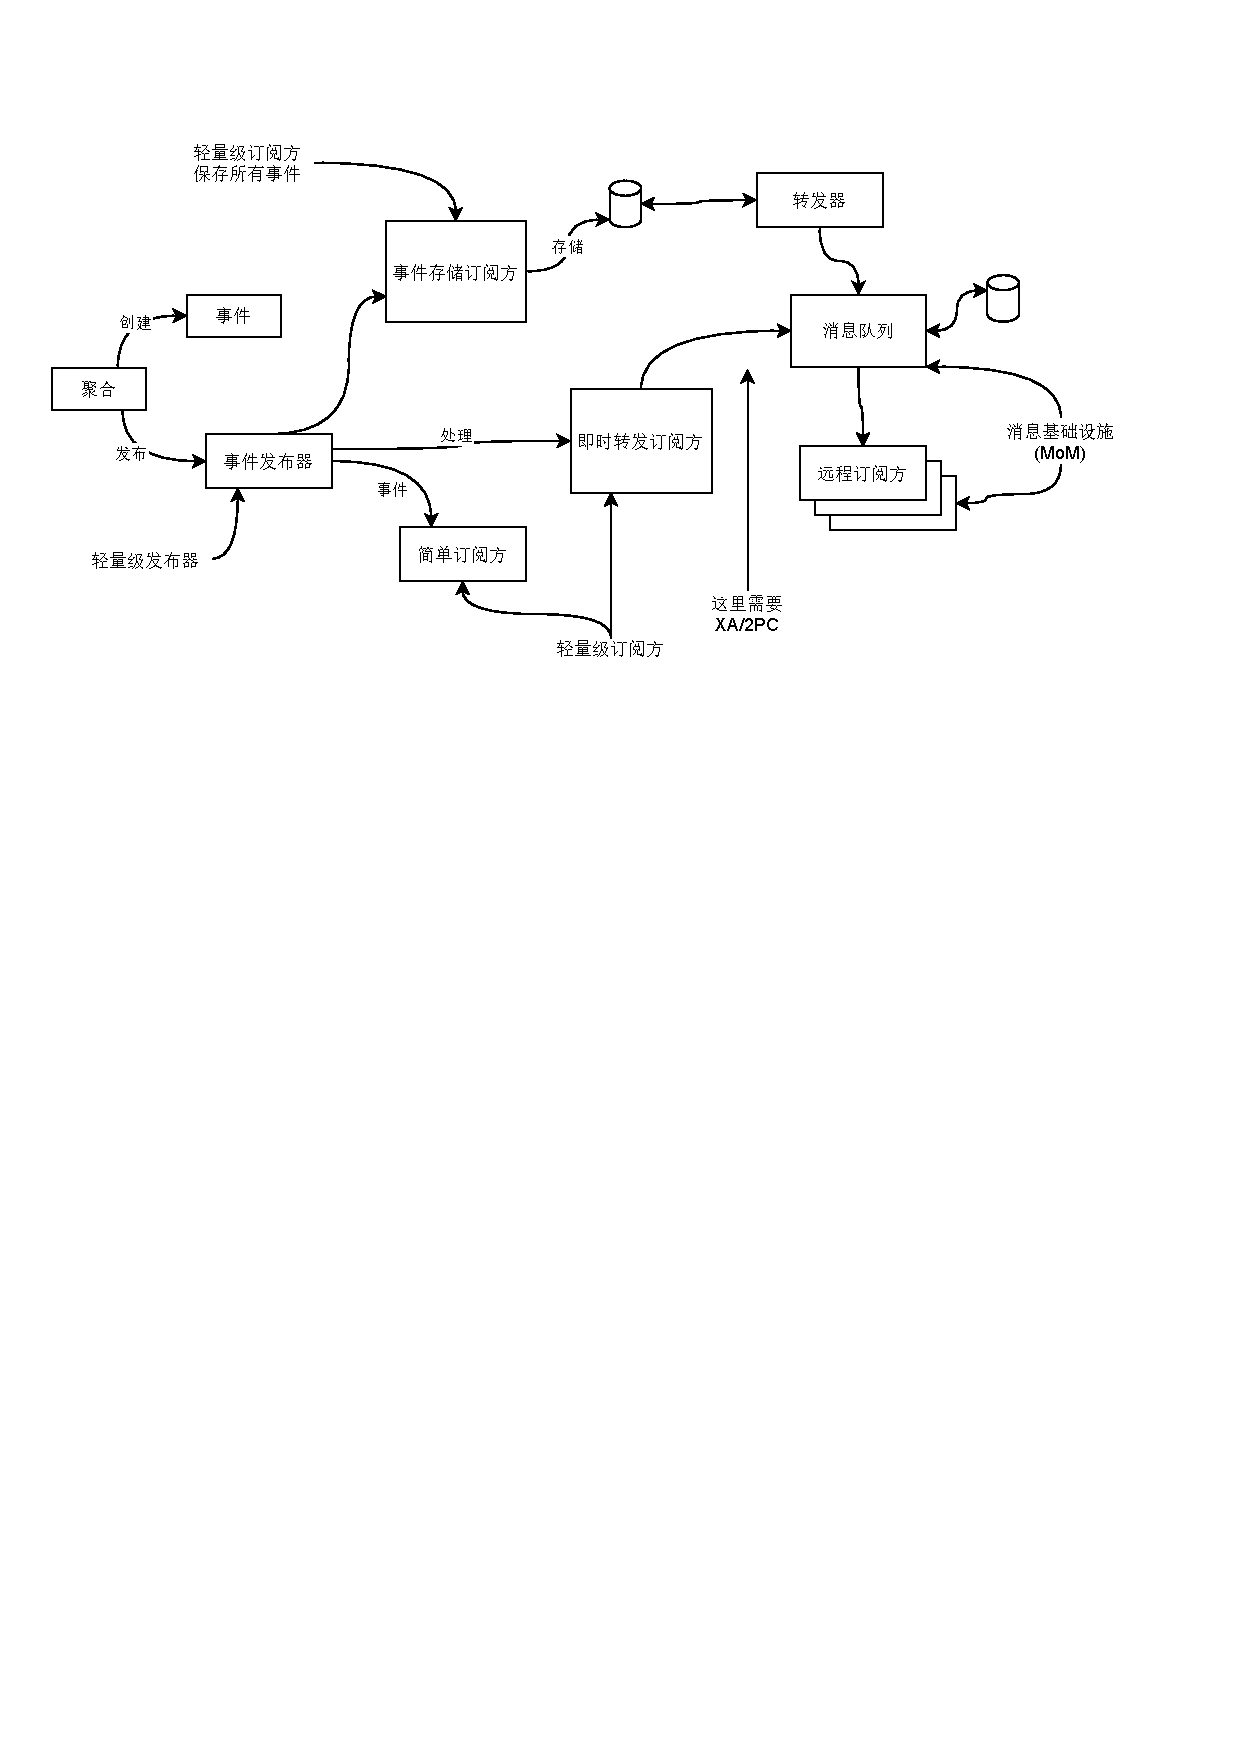
\includegraphics[width=0.8\textwidth]{FIGs/chapter3/DomainEventPractice.pdf} %中括号中的参数是设置图片充满文档的大小,你也可以使用小数来缩小图片的尺寸。
    \caption{领域事件实现流程图\protect\footnotemark[1]} %caption是用来给图片加上图题的
    \label{DomainEventPractice} %这是添加标签,方便在文章中引用图片。
\end{figure}%figure环境
\footnotetext[1]{图片来源于《实现领域驱动设计》}

P8:保持领域事件不变性
\begin{itemize}[leftmargin = 40pt]
    \item 只允许领域事件全状态初始化,避免初始化后又进行修改。
    \item 避免领域模型暴露到消息设施,防止第三方进行修改。
\end{itemize}

P9:转发领域事件
\begin{itemize}[leftmargin = 40pt]
    \item 通过RESTful接口发布。该方式适合多个客户同时通过相同URL请求来获取事件通知,不关注事件通知的顺序。
    \item 通过消息中间件方式发布。该方式依赖消息中间件省去细节处理,只需确保推送消息成功。
\end{itemize}

\textbf{模块实现技术及方案}

P10:组织模块
\begin{itemize}[leftmargin = 40pt]
    \item 不要只根据通用组件所属战术模式类型来组织模块,即不要简单地将所有聚合放在同一个模块,所有领域服务放在同一个模块,要考虑业务逻辑与行为。
    \item 设计松散耦合的模块,有利于维护和重构模块。
    \item 同层模块出现耦合时,杜绝循环依赖。
    \item 模块与建模对象一同变化,模型中对象改变时,模块也应进行改变。
\end{itemize}

\textbf{聚合实现技术及方案}

P11:保证一致性边界
\begin{itemize}[leftmargin = 40pt]
    \item 用事务来保证一致性边界。事务一致性要求立即性和原子性,提交单个事务时,聚合边界内的所有内容都必须保持一致。
\end{itemize}

P12:设计聚合的原则
\begin{itemize}[leftmargin = 40pt]
    \item 设计小聚合。使用根实体代表聚合,只包含最小数量的属性(需要在领域内保持一致性的属性)。
    \item 聚合内部建模成值对象。值对象可以配合根实体一同序列化存储,不会带来不必要的操作。
\end{itemize}

\textbf{资源库实现技术及方案}

P13:实现资源库
\begin{itemize}[leftmargin = 40pt]
    \item 为存储的聚合或实体提供访问的全局接口,确保存取的便捷性。
    \item 提供添加和删除方法。
    \item 提供顺序自增的唯一标识。
\end{itemize}

\subsection{战术建模指南构建结果}

本小节将介绍基于文献综述和访谈结果,
通过焦点小组讨论构建的战术建模指南。
指南中各模式包含的内容如表\ref{modelingframework}所示。
战术建模指南包含各个模式的名称、特征属性、使用时机和实现技术方案,
为方便表示,以上内容均以编号代表。


{\footnotesize
\begin{longtable}[h]{m{70pt}|m{125pt}|m{100pt}|m{75pt}}
    \caption[战术模式包含内容]{战术模式包含内容} \label{modelingframework} \\
        \hline  
        模式&属性&使用时机&实现技术\\
        \hline
        实体&CH1 CH2&T1 T2 T3&P1 P2 P3\\
        \hline
        值对象&CH3 CH4 CH5 CH6 CH7& T4 T5 &P4 P5\\
        \hline
        领域服务&CH8 CH9 CH10& T6 T7 &P6\\
        \hline
        领域事件&CH11 CH12 CH13 CH14&T8 T9&P7 P8 P9\\
        \hline
        模块&无&T10 T11&P10\\
        \hline
        聚合&CH15 CH16& T12 T13&P11 P12\\
        \hline
        资源库&CH17 CH18& T14 T15 T16& P13\\
        \hline

\end{longtable}
}

形成的具体战术建模指南如图\ref{theoryFramework}所示。
建模指南按模式划分,
每个模式包含了属性、实现技术及使用时机,
每个属性使用虚线关联其对应的实现技术。
为方便表示,以上内容均以编号代表。
该建模指南可以作为战术建模全流程的标准化参考。


\begin{figure}[!htbp] %figure环境,h默认参数是可以浮动,不是固定在当前位置。如果要不浮动,你就可以使用大写float宏包的H参数,固定图片在当前位置,禁止浮动。
    \centering %使图片居中显示
    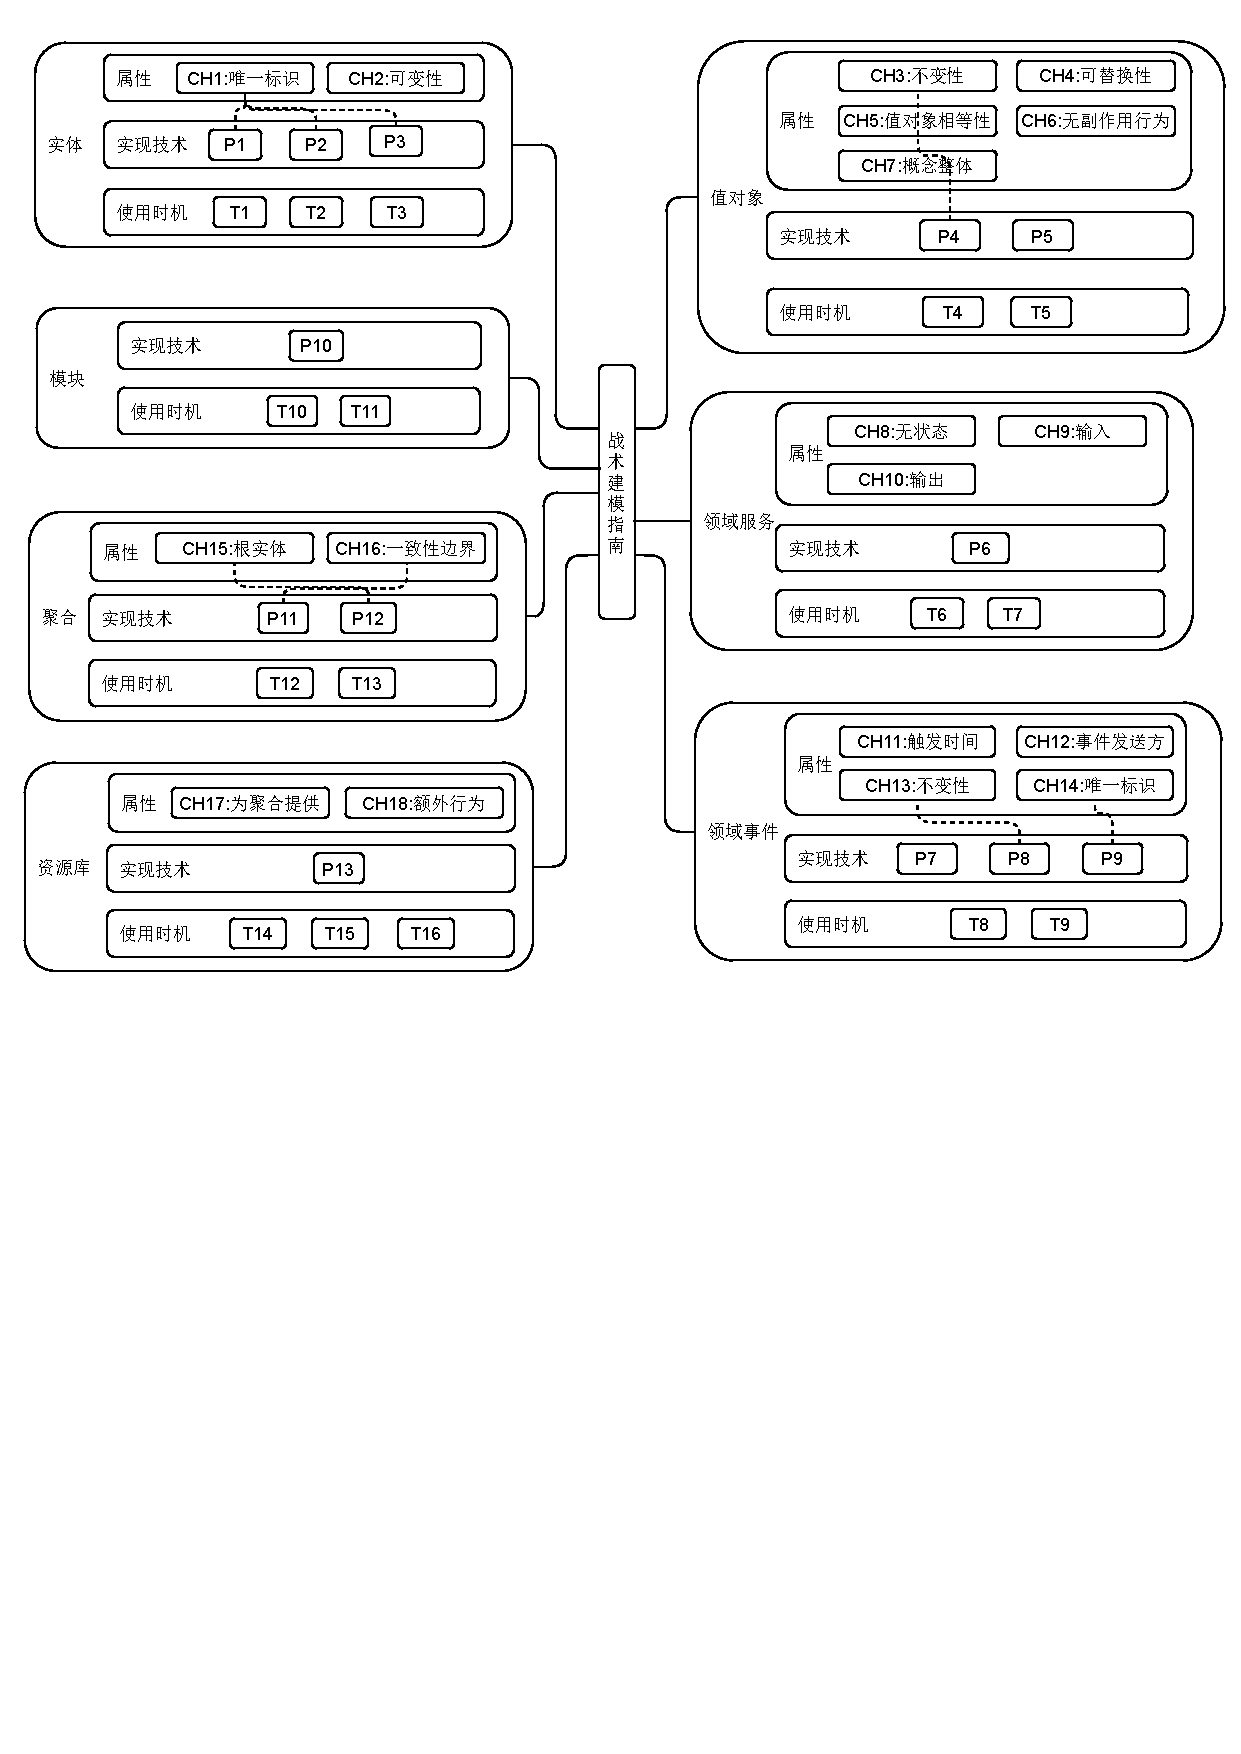
\includegraphics[width=0.8\textwidth]{FIGs/chapter3/theoryFramework.pdf} %中括号中的参数是设置图片充满文档的大小,你也可以使用小数来缩小图片的尺寸。
    \caption{战术建模指南} %caption是用来给图片加上图题的
    \label{theoryFramework} %这是添加标签,方便在文章中引用图片。
\end{figure}%figure环境

\section{战术建模语言}

% 战术建模框架本身应该是基于review和访谈结果总结得到的一个战术建模方法,想想看它应该包含哪些内容

本节将介绍基于焦点小组讨论实例化的战术建模语言。
作者实例化建模语言的过程参考了\cite{giachetti2009integration,giachetti2009using}文献中的流程方法,
提出的元模型参考了\cite{hippchen2019systematic,le2018domain,rademacher2017towards}文献中的现有元模型。
首先使用UML profile机制来进行战术建模元模型的构建,
包括战术建模初始元素集的构建,
初始元素集展示了建模语言中需要使用的重要概念,
并与元类类型对应;
还构建了战术建模元类,
UML中的元类是一种成熟的元模型实现方式,
由于UML类图与软件设计实现关系密切,并且易于阅读理解,
所以以其为重点进行UML profile的构建;
然后使用对象约束语言(OCL)对约束条件进行实现,
对象约束语言(OCL)是一种施加在指定模型元素上的约束语言,
为元模型附加了更多约束条件使其更加完善。


\subsection{战术建模语言元素集}

根据表\ref{table:patterns}定义战术建模UML profile元模型(Metamodel)需要的元素集。
本文定义的元素集如表\ref{ProfileElementSet}所示,
表中展示了元素集中元素的名称,代表的元类类型以及描述。

{\footnotesize
\begin{longtable}[h]{m{80pt}|m{90pt}|m{205pt}}
\caption[战术建模profile元素集]{战术建模profile元素集} \label{ProfileElementSet} \\
    \hline  
    元素名&元类类型&描述\\
    \hline
    Entity&Class&实体是一个由标识符定义的对象,通过标识符与其他对象区别开来确保其个性特征。\\
    \hline
    ValueObject&Class&值对象用来度量和描述事物,具有不可变性。\\
    \hline
    DomainService&Class&领域服务是一个独立接口或对象,负责承担不属于实体或值对象职责的操作或转换过程。\\
    \hline
    DomainEvent&Class&领域事件记录了领域中发生的事情,无法改变,还可以维护发布到外部上下文的业务一致性。\\
    \hline
    AggregateRoot&Class&聚合是一个将实体和值对象聚类到一致性边界内的容器,每个聚合内部有一个实体作为聚合根,
    聚合通过聚合根与外部进行交互。\\
    \hline
    Repository&Class&资源库是一个用来存取领域对象的安全存储区域,还可以提供对象的存取、删除和查询操作。\\
    \hline
    DefineIdentity&Property or Operation&唯一标识,用来区分其他对象和跟踪对象。\\
    \hline
    Module&Package&模块是用来存放内聚类的容器,主要用在技术层面的代码组织、构建目录与打包。\\
    \hline
    Input&Class and Property&领域服务对象或领域事件对象方法的输入。\\
    \hline
    Output&Class and Property&领域服务对象方法的输出。\\   
    \hline
    OccurTime&Property&领域事件触发时间。\\
    \hline
    EventStep&Property or Operation&事件步骤,用来描述领域事件。\\
    \hline
    ACL&Class&防腐层,用来和其他上下文交互和隔离。\\
    \hline
\end{longtable} 
}

如表\ref{ProfileElementSet}所示,在重要战术模式表\ref{table:patterns}的基础上,
进行了优化与修改。
直接用聚合根(AggregateRoot)和与聚合根直接或间接相连的所有对象表示聚合(Aggregate),
为领域服务(Domain Service)引入必要属性输入(Input)和输出(Output),
为领域事件(Domain Event)引入必要属性输入(Input)来代表发送方,
还引入了触发时间(OccurTime)和领域事件步骤(EventStep)属性。
引入严格意义上不是战术模式但可能会用到的概念元素防腐层(Anti-Corruption Layer,ACL)。

\subsection{战术建模元类}

一个UML profile包含构造型(Stereotypes)形式的UML元类的扩展,
还包含元类中类(Class)、属性(Property)和操作(Operation)的映射关系
\cite{files2013omg},
使用定义好的配置文件构造型,可以对元类进行扩展,丰富其语义。
如图\ref{metaclass}描述了扩展元类的战术建模UML profile,包含所有的构造型,
以及各构造型之间的包含关系,采用标记值(Tagged Values)进行表示。
其中,箭头表示构造型扩展自元类。

\begin{figure}[!htb] %figure环境,h默认参数是可以浮动,不是固定在当前位置。如果要不浮动,你就可以使用大写float宏包的H参数,固定图片在当前位置,禁止浮动。
    \centering %使图片居中显示
    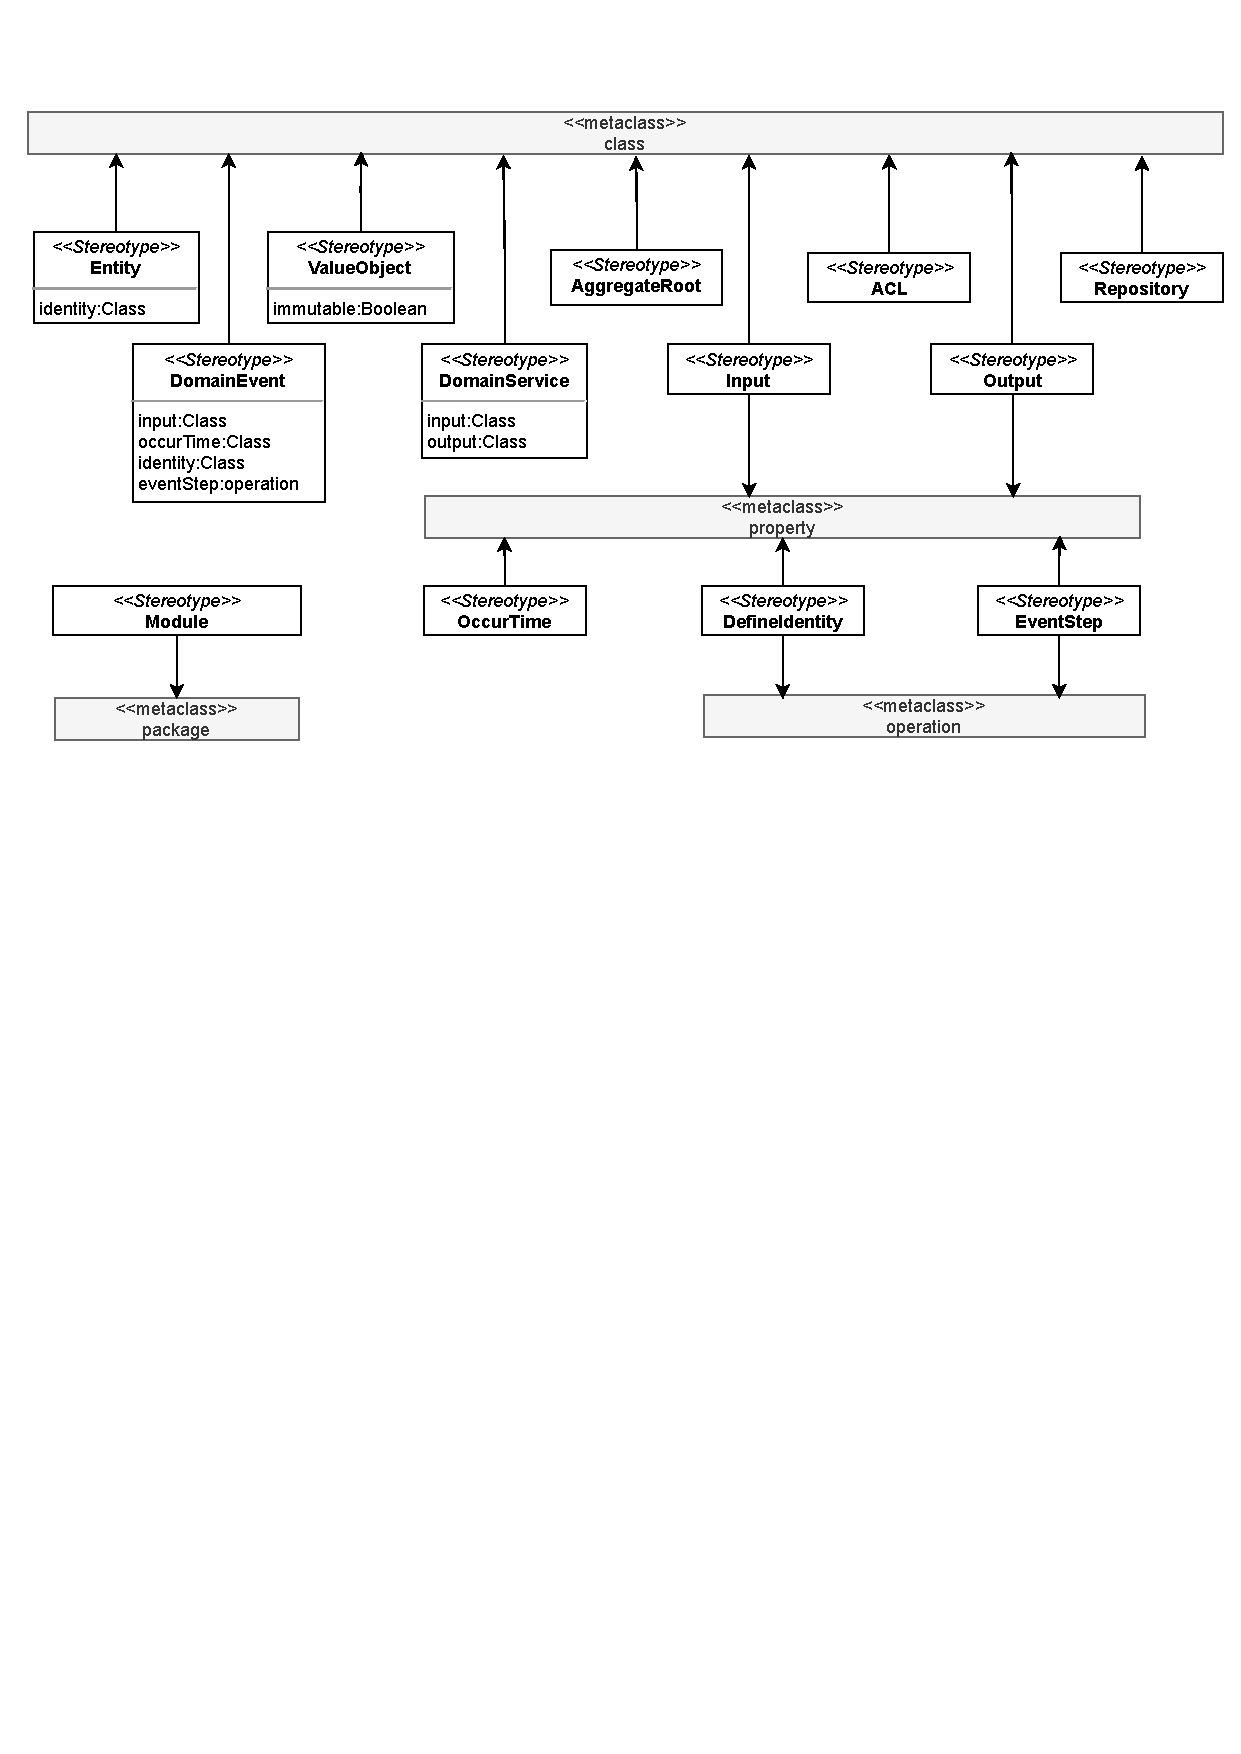
\includegraphics[width=0.8\textwidth]{FIGs/chapter3/metaclass.pdf} %中括号中的参数是设置图片充满文档的大小,你也可以使用小数来缩小图片的尺寸。
    \caption{战术建模扩展元类profile} %caption是用来给图片加上图题的
    \label{metaclass} %这是添加标签,方便在文章中引用图片。
\end{figure}%figure环境

\subsection{战术建模语言约束}

为元类添加约束可以防止不规范或错误使用元类,
为确保上述扩展元类正常使用以及建模过程的准确性,
每个元类都被添加了相应约束,具体约束如表\ref{stereotypeconstraint}所示,
使用英文单词“Constraint”的大写首字母“C”结合序号对约束进行编号,
并通过对象约束语言对约束进行标准化的实现。

% 结合profile的拓展机制形成的元模型
% 特征,约束和规则,表格形式

{\footnotesize
\begin{longtable}[h]{m{90pt}|m{295pt}}
    \caption[构造型约束规则]{构造型约束规则} \label{stereotypeconstraint} \\
        \hline  
        构造型&约束\\
        \hline
        Entity&C1:实体必须拥有一个方法或属性定义唯一标识。\\
        \hline
        DomainService&C2:领域服务类不能具有其他构造型。
        \newline C3:领域服务必须拥有输入值。
        \newline C4:领域服务必须拥有输出值。\\
        \hline
        DomainEvent&C5:领域事件类不能具有其他构造型。
        \newline C6:领域事件必须记录被触发时间。
        \newline C7:领域事件必须拥有事件发送方作为输入。
        \newline C8:领域事件必须拥有唯一标识来跟其他对象进行区分。\\
        \hline
        AggregateRoot&C9:只有实体能充当聚合根并与其他聚合根连接。
        \newline C10:一个聚合根只能由一个实体代表。\\
        \hline
        Repository&C11:资源库类不能具有其他构造型。
        \newline C12:只为实体或聚合根提供资源库。
        \newline C13:资源库只定义方法,且至少定义一个方法。
        \\
        \hline
        ValueObject&C14:值对象不可变。\\
        \hline
        DefinesIdentity&C15:唯一标识可以以属性或方法返回值的形式存在于对象中。
        \newline C16:唯一标识必须在实体或领域事件中使用。\\
        \hline
        Input&C17:输入以属性形式存在于对象中,且必须指定输入代表的对象。\\
        \hline
        Output&C18:输出以属性形式存在于对象中,且必须指定输出代表的对象。\\   
        \hline
        OccurTime&C19:触发时间必须作为属性在领域事件中使用。\\
        \hline
    \end{longtable} 
}
% 使用OCL时运用到了以JavaScript\footnote{JavaScript主页:https://www.javascript.com/}
% 为基础的开源工具包OCL.js\footnote{OCL.js开源项目仓库:https://github.com/SteKoe/ocl.js}。
% 使用该工具后,可以直接将OCL语句集成到前端项目代码中,达到校验约束、方便查看的效果。
对象约束语言(OCL)可以施加在指定元类上,
为元类附加更多约束条件,
使其在使用过程中更加标准规范,避免错误地使用元类。
由于本文篇幅有限,仅选择领域事件的约束实现进行展示,
如图\ref{DomainEventOCL}所示,展示了用OCL实现的领域事件约束。\\

\begin{figure}[!htbp] %figure环境,h默认参数是可以浮动,不是固定在当前位置。如果要不浮动,你就可以使用大写float宏包的H参数,固定图片在当前位置,禁止浮动。
    \centering %使图片居中显示
    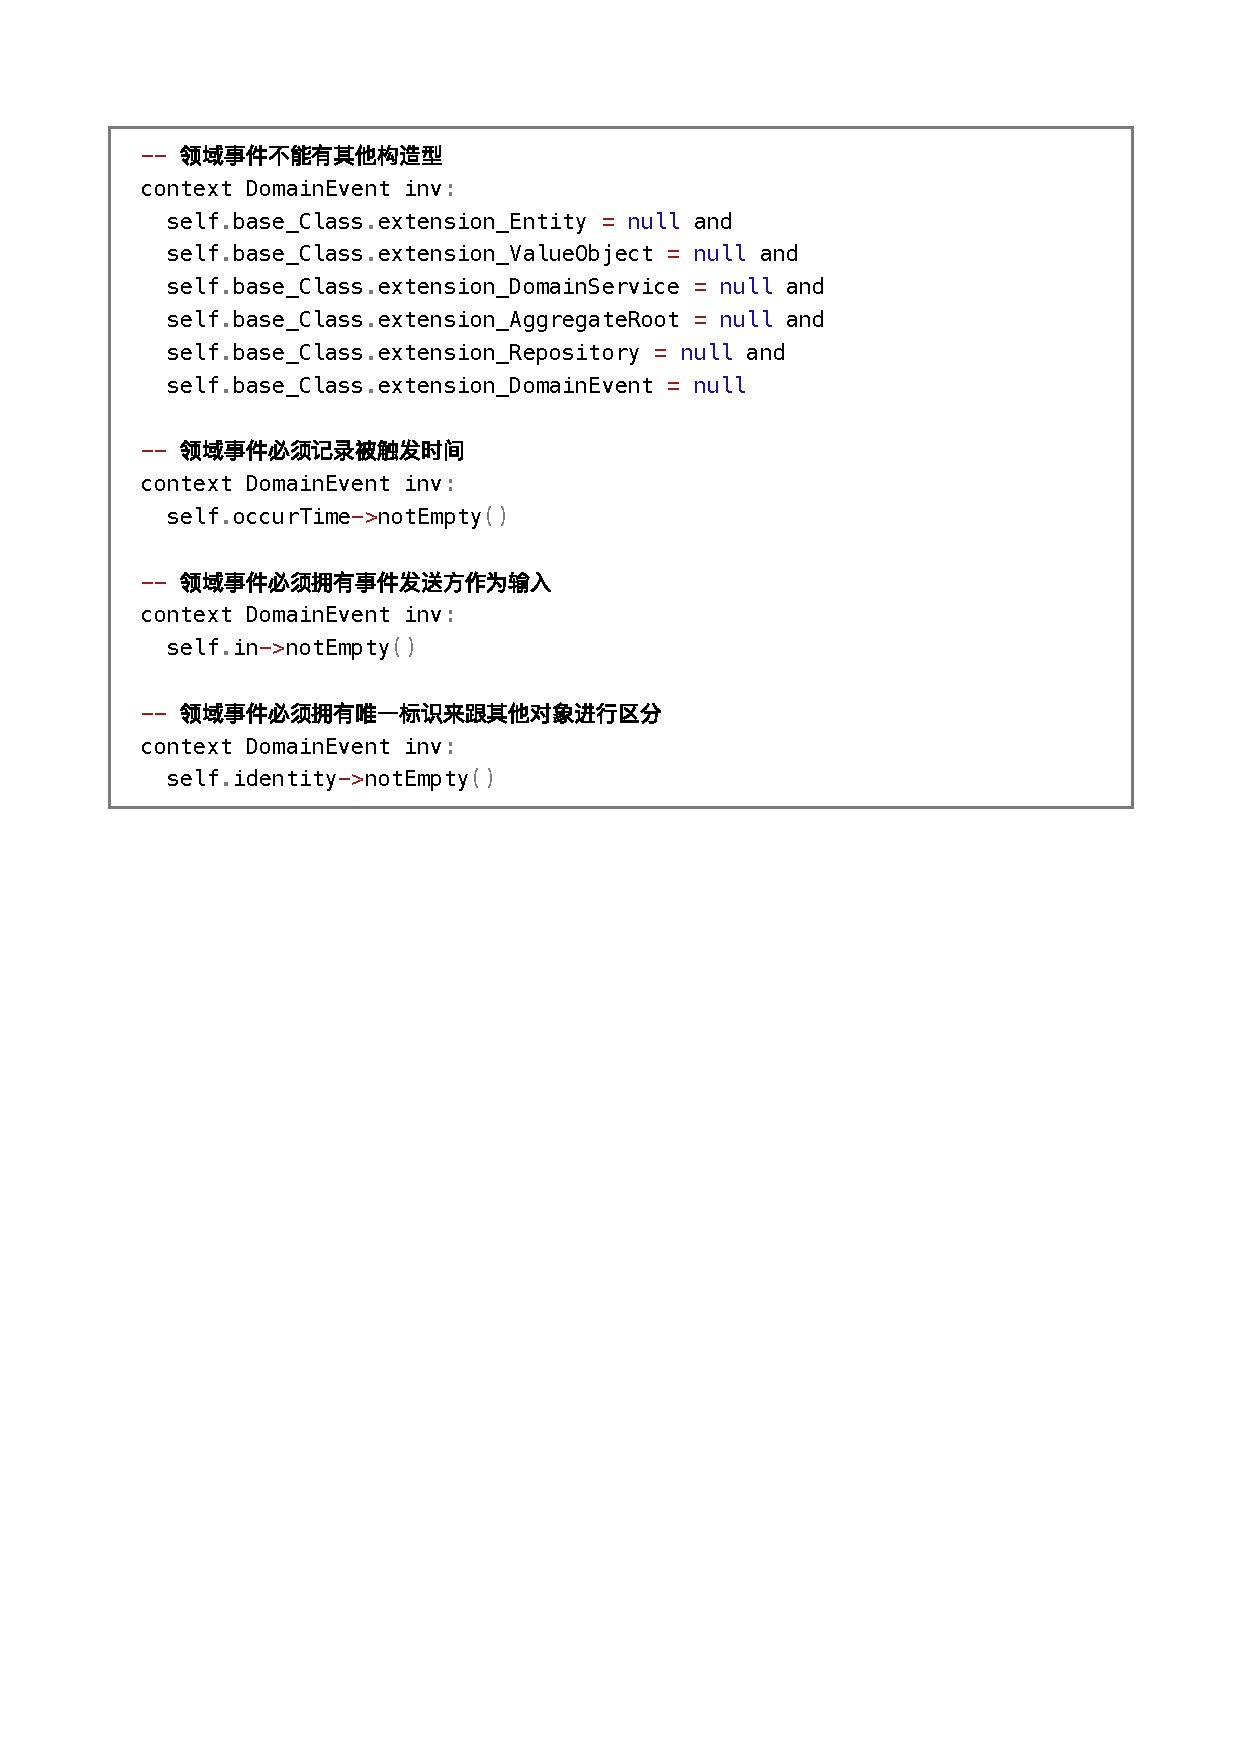
\includegraphics[width=0.8\textwidth]{FIGs/chapter3/DomainEventOCL.pdf} %中括号中的参数是设置图片充满文档的大小,你也可以使用小数来缩小图片的尺寸。
    \caption{DomainEvent约束实现} %caption是用来给图片加上图题的
    \label{DomainEventOCL} %这是添加标签,方便在文章中引用图片。
\end{figure}%figure环境

% \subsection{战术建模最佳实践经验}


% \subsection{支持工具}

% 支持框架的工具使用流程如下图\ref{toolprocess}所示。
% 开发者使用支持工具开始建模,首先可以选择学习或回顾DDD基本概念知识,
% 为后续建模做理论准备,也可以继续从上一次建模保存的结果开始继续建模;
% 进行可视化建模时,开发者可以随时进行对建模结果的验证,
% 工具将对不符合规范的建模结果给出提示和警告;如果建模结果符合规范和约束,
% 工具将保存建模结果到数据库,通过工具可以将建模结果以XML、图片或Json格式导出;
% 最后,还可以根据建模结果生成框架项目文件。

% \begin{figure}[h] %figure环境,h默认参数是可以浮动,不是固定在当前位置。如果要不浮动,你就可以使用大写float宏包的H参数,固定图片在当前位置,禁止浮动。
%     \centering %使图片居中显示
%     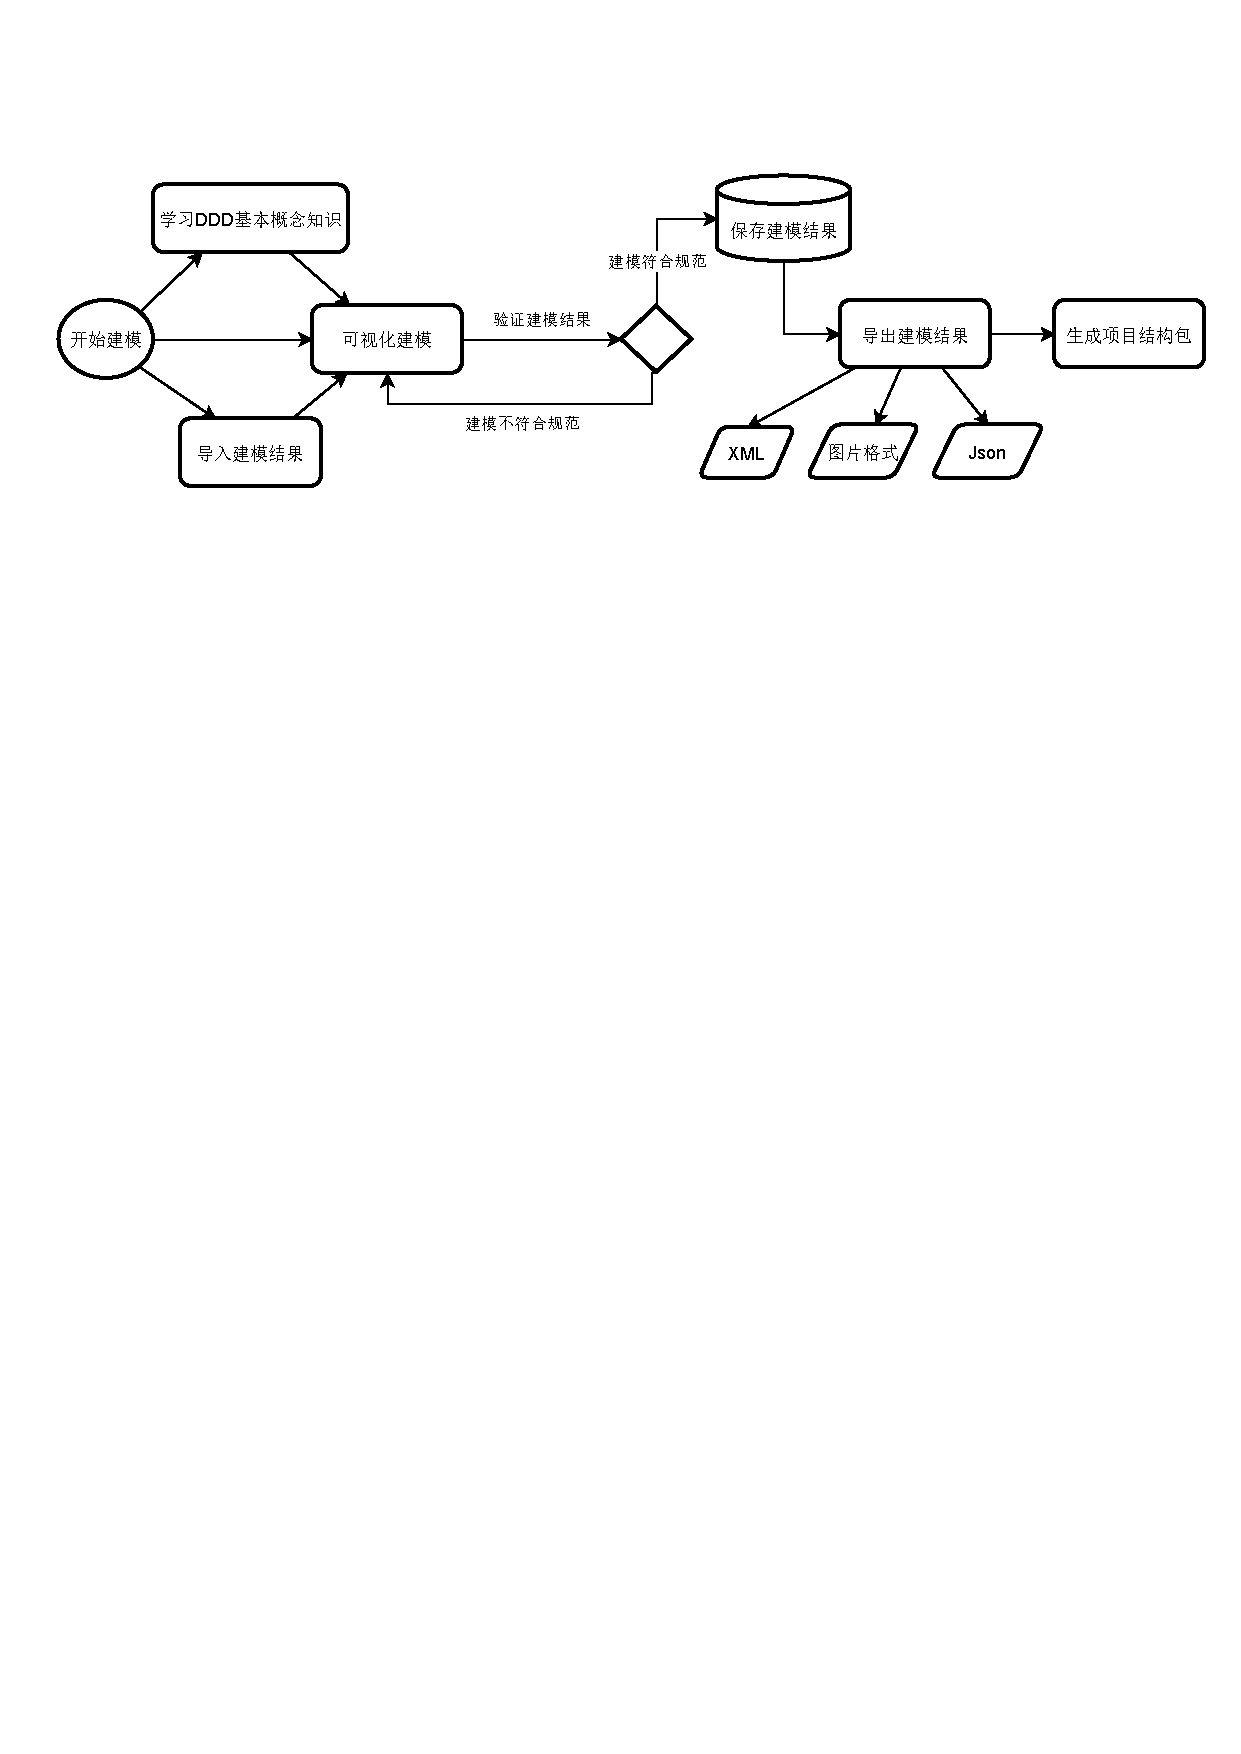
\includegraphics[width=0.8\textwidth]{FIGs/chapter3/toolprocess.pdf} %中括号中的参数是设置图片充满文档的大小,你也可以使用小数来缩小图片的尺寸。
%     \caption{框架支持工具业务流程} %caption是用来给图片加上图题的
%     \label{toolprocess} %这是添加标签,方便在文章中引用图片。
% \end{figure}%figure环境

\section{本章小结}

本章介绍了提出战术建模支持方法的研究过程及其结果。
其中研究过程包括文献综述、访谈和焦点小组,
文献综述部分对前期收集理论知识的目的和过程进行介绍,并为访谈和构建支持方法做准备工作;
访谈部分依据文献综述的成果,设计了问卷并对工业界内的领域驱动设计实践者进行访谈;
访谈后的初步产物作为焦点小组的输入,通过多次讨论,构建了战术建模支持方法。
研究结果包括由文献综述和访谈得到的战术建模指南,
即战术模式及属性、战术模式使用时机和实现技术;
还包括焦点小组讨论得出的战术建模语言。
上述战术建模指南和战术建模语言共同组成了本文提出的战术建模支持方法。






\chapter{建模支持工具设计与实现}

\section{概述}

战术建模在分析与设计阶段一直缺少一个标准化、规范化的流程指导,
许多设计过程停留在使用纸和笔简单勾画草稿的阶段,
即使是建模经验丰富的架构师,也无法保证战术建模结果的统一性。
开发人员缺少对领域的理解,甚至对战术模式的使用也不够熟悉,
导致投入战术建模的精力无法得到相应回报。

因此,一个支持标准化、规范化战术建模的工具十分重要。
本章基于第三章提出的战术建模支持方法中的战术建模语言,
提供配套的可视化建模工具DDDD(Draw for Domain-Driven Design)来支撑实现战术建模。
建模工具DDDD应具备简单的建模知识介绍,方便使用者快速获取战术建模知识,
并运用到分析设计中;
还应具有“可视化建模”模块,该模块支持依据本文提出的战术建模元模型进行可视化建模,
通过灵活的拖拽和点击,即可完成战术建模过程,
帮助架构师和开发人员更加灵活高效地进行战术建模;
还应具有“模型校验”模块,该模块支持对建模结果的验证,用于检测建模的结果是否符合第三章中提出的战术建模元模型,
并给出修改意见,保证建模结果的规范性和正确性;
最后,还应具有“模型存储与转化”模块,该模块支持将建模结果进行存储,方便后续访问和修改,保证了建模结果的可复用性,
支持对建模结果进行扩展,生成符合领域驱动设计标准的框架项目代码包,
为实现阶段提供良好开端。

本章实现的建模支持工具使用流程如下图\ref{toolprocess}所示。
开发人员或架构师使用支持工具开始建模,
首先可以通过“模型存储与转化”模块的模型加载功能继续从上一次建模保存的结果开始继续建模;
使用“可视化建模”模块进行建模时,
开发人员或架构师可以随时使用“模型校验”模块进行对建模结果的验证,
确保建模的正确性和规范性,
工具也将对不符合规范的建模结果给出提示和警告,帮助开发人员和架构师进行修改;
如果建模结果符合规范和约束,工具将通过“模型存储与转化”模块保存建模结果到数据库, 
或者以 XML、图片或 JSON 格式导出,还可以根据建模结果生成框架项目文件。


\begin{figure}[!htbp] %figure环境,h默认参数是可以浮动,不是固定在当前位置。如果要不浮动,你就可以使用大写float宏包的H参数,固定图片在当前位置,禁止浮动。
    \centering %使图片居中显示
    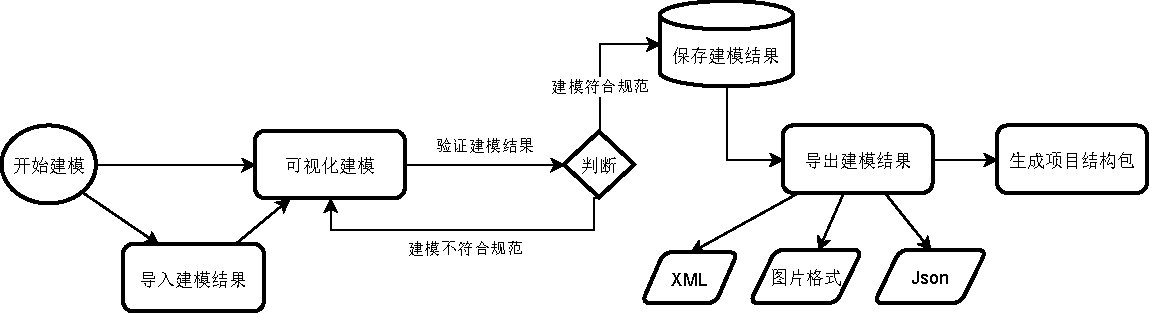
\includegraphics[width=0.8\textwidth]{FIGs/chapter4/toolprocess.pdf} %中括号中的参数是设置图片充满文档的大小,你也可以使用小数来缩小图片的尺寸。
    \caption{建模支持工具业务流程} %caption是用来给图片加上图题的
    \label{toolprocess} %这是添加标签,方便在文章中引用图片。
\end{figure}%figure环境



本章的剩余部分将对建模支持工具进行需求分析,
根据分析得到的结果对工具进行设计与实现。
首先对工具按功能模块进行划分,按模块介绍功能需求与非功能性需求;
然后对工具进行总体设计;最后介绍各模块详细设计与实现。


\section{需求分析}

\subsection{工具总体功能}

DDDD(Draw for Domain-Driven Design)建模支持工具总体功能规划
如图\ref{toolstotal}所示,
主要包括“可视化建模”模块、“模型校验”模块以及“模型存储与转化”模块,
各模块详细功能需求描述如下:

\begin{figure}[!htbp] %figure环境,h默认参数是可以浮动,不是固定在当前位置。如果要不浮动,你就可以使用大写float宏包的H参数,固定图片在当前位置,禁止浮动。
    \centering %使图片居中显示
    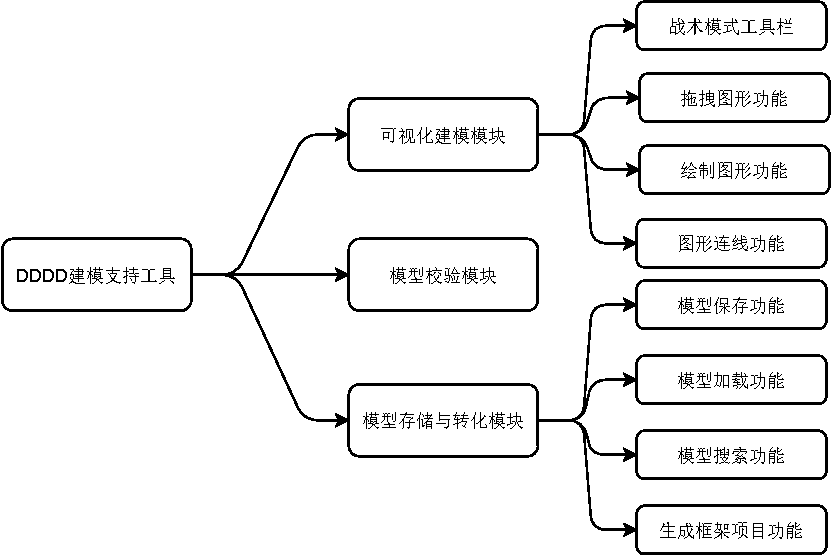
\includegraphics[width=0.8\textwidth]{FIGs/chapter4/toolstotal.pdf} %中括号中的参数是设置图片充满文档的大小,你也可以使用小数来缩小图片的尺寸。
    \caption{工具总体功能} %caption是用来给图片加上图题的
    \label{toolstotal} %这是添加标签,方便在文章中引用图片。
\end{figure}%figure环境


% \begin{figure}[!htbp] %figure环境,h默认参数是可以浮动,不是固定在当前位置。如果要不浮动,你就可以使用大写float宏包的H参数,固定图片在当前位置,禁止浮动。
%     \centering %使图片居中显示
%     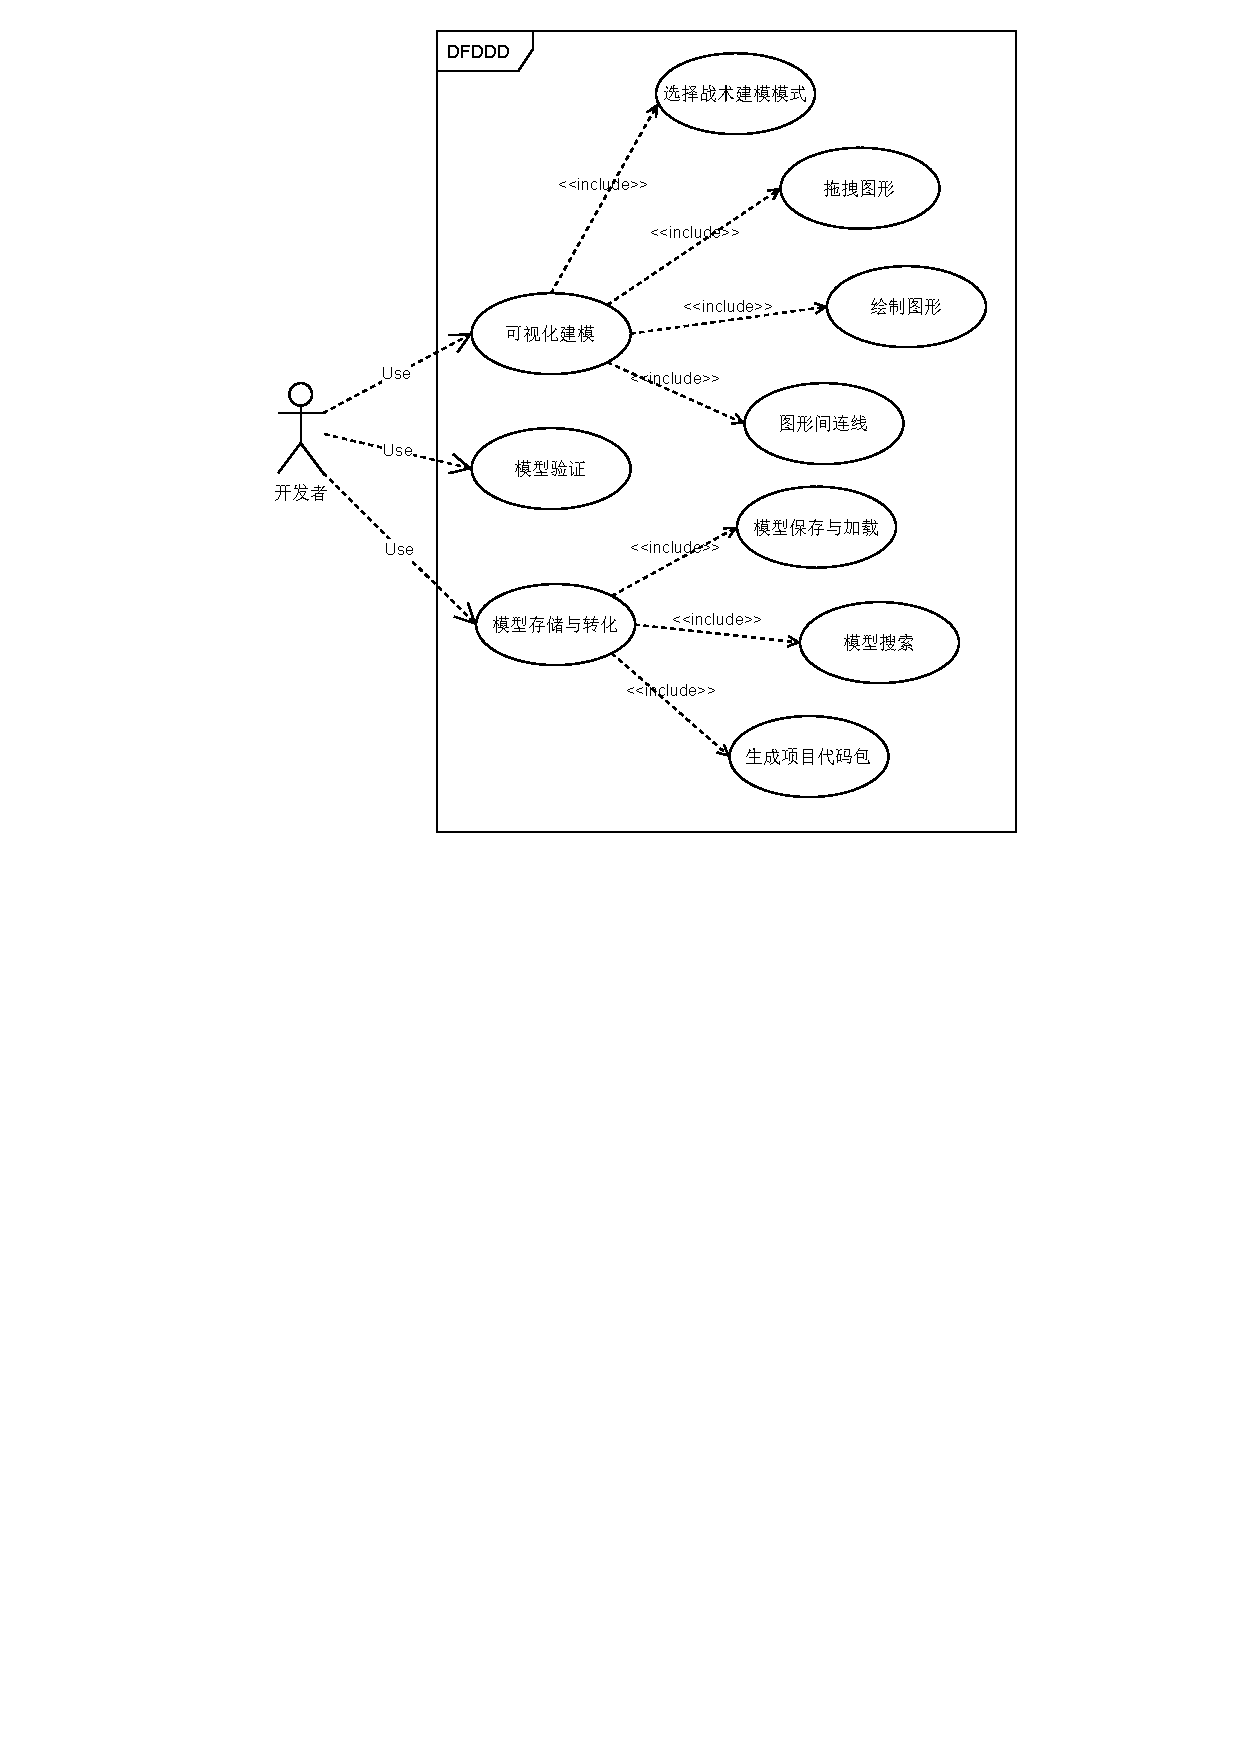
\includegraphics[width=0.8\textwidth]{FIGs/chapter4/usecaseDFDDD.pdf} %中括号中的参数是设置图片充满文档的大小,你也可以使用小数来缩小图片的尺寸。
%     \caption{建模支持工具用例图} %caption是用来给图片加上图题的
%     \label{usecaseDFDDD} %这是添加标签,方便在文章中引用图片。
% \end{figure}%figure环境

\begin{itemize}
    \item “可视化建模”模块:支持开发人员从工具栏中选择需要使用的战术模式,并灵活地将
    模式图形拖拽到建模绘图面板上进行绘制,还支持根据建模需要对不同的模式进行连线,
    表达模式间的关系,完成可视化建模过程。
    \item “模型校验”模块:在建模过程中或建模完成时,可以依据定义的战术建模元模型中的约束
    对建模的结果进行验证,并给出修改意见。
    \item “模型存储与转化”模块:建模完成后,将建模结果进行存储或导出到本地,
    也可以从数据库或本地读取模型文件,根据建模结果,生成符合领域驱动设计规范的框架项目代码包。

\end{itemize}

\subsection{可视化建模模块需求分析}

\textbf{功能性需求}

“可视化建模”模块是本建模支持工具的核心功能模块,
如图\ref{us1}所示,
开发人员或架构师可以通过“可视化建模”模块“选择战术建模模式”、“拖拽图形”、
“绘制图形”以及进行“图形间连线”。

\begin{figure}[!htbp] %figure环境,h默认参数是可以浮动,不是固定在当前位置。如果要不浮动,你就可以使用大写float宏包的H参数,固定图片在当前位置,禁止浮动。
    \centering %使图片居中显示
    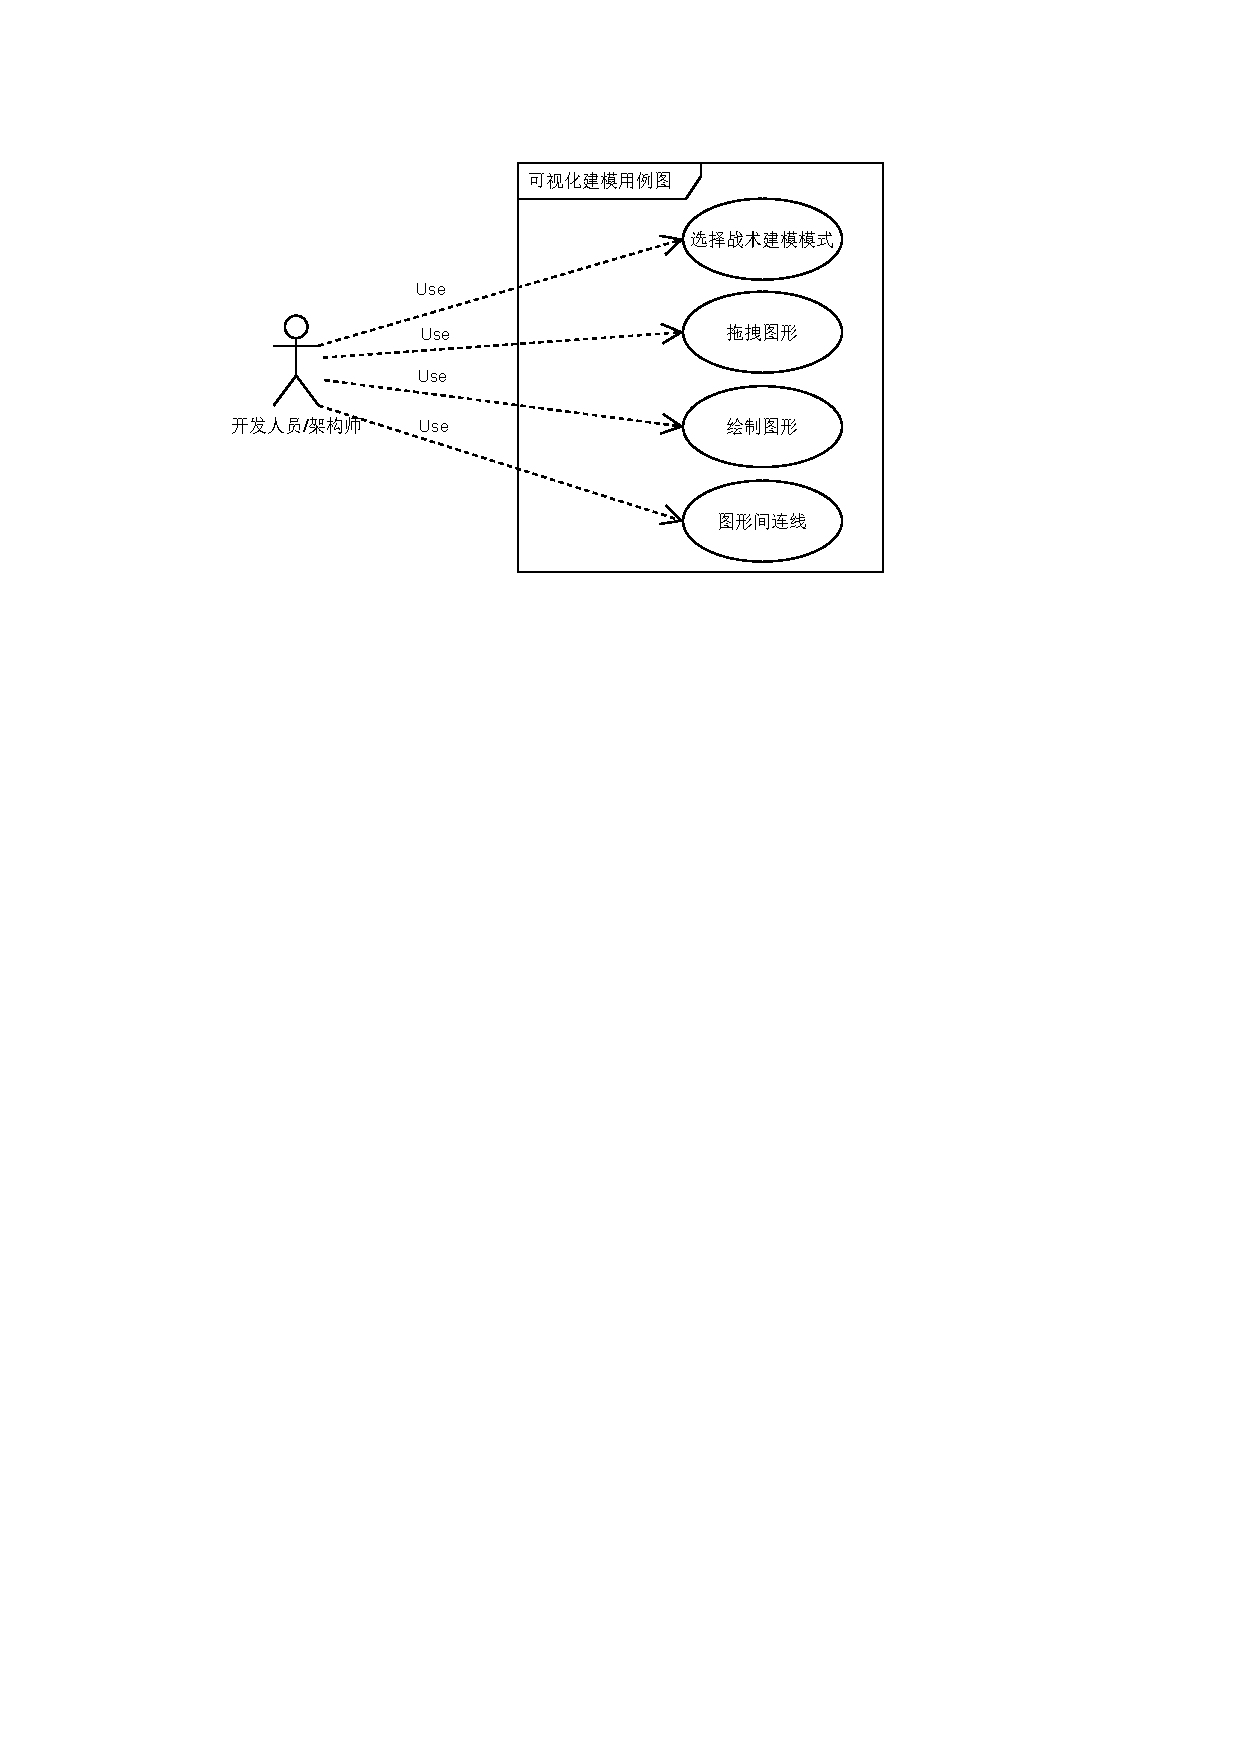
\includegraphics[width=0.8\textwidth]{FIGs/chapter4/us1.pdf} %中括号中的参数是设置图片充满文档的大小,你也可以使用小数来缩小图片的尺寸。
    \caption{可视化建模模块用例图} %caption是用来给图片加上图题的
    \label{us1} %这是添加标签,方便在文章中引用图片。
\end{figure}%figure环境

表\ref{usecase1}展示了“可视化建模”模块的用例描述,
“可视化建模”为开发者提供灵活方便的可拖拽式建模方式,
可以自由选择需要使用的战术模式,拖拽到绘制面板中进行绘制,
对绘制的模型对象可以双击修改文字信息,并将当前模型对象与其他对象进行连线,
以表示它们之间的关系,在绘制面板上方还有以按钮形式提供的绘图操作菜单。

{\footnotesize
\begin{longtable}[h]{m{80pt}|m{305pt}}
    \caption[可视化建模用例表]{可视化建模用例表} \label{usecase1} \\
        \hline  
        ID&UC1\\
        \hline
        名称&可视化建模用例\\
        \hline
        描述&开发者使用工具可以拖拽式地进行建模,选择战术模式相应图形化模型,
        拖拽到建模绘制面板中,并修改模型对象信息、对象间关系,达到灵活可视化建模。\\
        \hline
        触发条件&从主页点击“开始建模”按钮\\
        \hline
        前置条件&用户浏览器支持JavaScript\\
        \hline
        后置条件&无\\
        \hline
        正常流程& (1)用户点击“开始建模”按钮;
        \newline (2)用户点击展开战术模式列表,拖拽需要的模式进入绘图面板;
        \newline (3)松开鼠标,模型对象绘制完成,双击模型对象文字块,修改文字信息;
        \newline (4)当鼠标悬停在模型对象上且边框变绿,按住鼠标左键拖动绘制箭头,
                    连接到其他模型对象上;
        \newline (5)点击绘图板上方按钮可对模型进行验证、组合、分解、删除、撤销以及缩放画布操作。\\
        \hline
        异常流程&无\\
        \hline
    \end{longtable} 
}

\textbf{非功能性需求}

“可视化建模”模块的非功能性需求主要包括易用性、可靠性和可扩展性,
具体需求如下:

\begin{itemize}
    \item 易用性:可视化的建模过程易于学习和使用,
    用户仅需进行简单的拖拉拽操作即可完成图形化建模,
    速度快,图形变换灵活简单,建模结果清晰明确,符合用户建模的期望。

    \item 可靠性:在“可视化建模”过程中,绘图逻辑大多都在前端完成,
     即使网络连接断开也不影响建模过程,保障了建模过程的连贯性。
   
     \item 可扩展性:“可视化建模”的战术模式工具栏可以根据需求添加和删除战术模式,
     适应未来战术建模理论的更新和发展。
\end{itemize}

\subsection{模型校验模块需求分析}

\textbf{功能性需求}

“模型校验”模块用例图如图\ref{us2}所示,
该模块帮助开发人员或架构师根据元模型和约束规则对建模结果进行验证和修改。

表\ref{usecase2}展示了"模型校验"功能模块的用例描述,
“模型校验”根据本文定义的战术建模元模型约束规则和图形绘制规则对图形化的建模结果
进行验证,对不符合规范和约束的模型进行警告和给出修改提示,
对验证通过的模型进行命名并保存到数据库中。

\begin{figure}[!htbp] %figure环境,h默认参数是可以浮动,不是固定在当前位置。如果要不浮动,你就可以使用大写float宏包的H参数,固定图片在当前位置,禁止浮动。
    \centering %使图片居中显示
    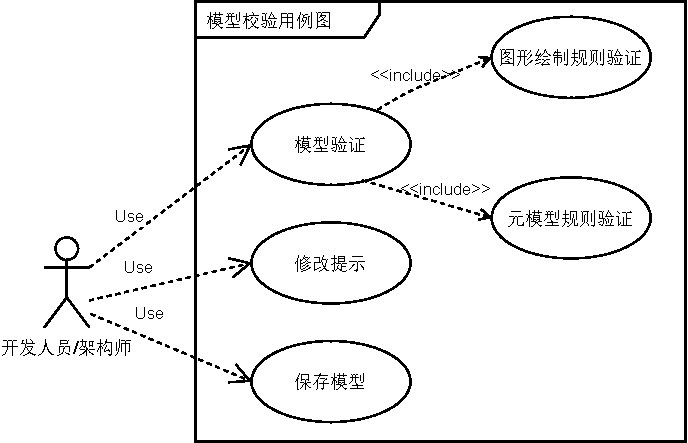
\includegraphics[width=0.8\textwidth]{FIGs/chapter4/us2.pdf} %中括号中的参数是设置图片充满文档的大小,你也可以使用小数来缩小图片的尺寸。
    \caption{模型校验模块用例图} %caption是用来给图片加上图题的
    \label{us2} %这是添加标签,方便在文章中引用图片。
\end{figure}%figure环境


{\footnotesize
\begin{longtable}[h]{m{80pt}|m{305pt}}
    \caption[模型校验用例表]{模型校验用例表} \label{usecase2} \\
        \hline  
        ID&UC2\\
        \hline
        名称&模型校验\\
        \hline
        描述&根据本文提出的战术建模元模型及约束规则对建模结果进行验证,
        并给出修改意见\\
        \hline
        触发条件&绘图界面点击“验证”按钮\\
        \hline
        前置条件&建模进行中或已经完成\\
        \hline
        后置条件&无\\
        \hline
        正常流程& (1)当建模面板不为空时,开发者点击“验证”按钮;
        \newline (2)前端界面弹出验证通过或验证失败及修改提示信息;
        \newline (3)如果验证通过,将建模结果命名并自动保存在数据库中。\\
        \hline
        异常流程&保存建模结果时未填写名称,提示填写\\
        \hline
    \end{longtable} 
}

\textbf{非功能性需求}

“模型校验”模块的非功能性需求主要包括易用性、健壮性和可靠性,
具体需求如下:

\begin{itemize}
    \item 易用性:模型的验证结果以弹窗形式展示,
    指出建模不规范的地方并给出修改建议,
    让用户明确需要修改哪些建模结果。

    \item 健壮性:验证操作能够应对各种异常情况并作出响应。
    对于错误输入、非法字符和误操作等能够规避和纠正,
    有效防止建模过程中工具的崩溃。
   
     \item 可靠性:支持每次验证操作都将建模结果自动保存到数据库,
    保障了建模结果不丢失和及时更新持久化内容。
\end{itemize}

\subsection{模型存储与转化模块需求分析}

“模型存储与转化”模块用例图如图\ref{us3}所示,
开发人员或架构师通过“模型存储与转化”模块对模型进行导入和导出,
对数据库中存储的模型进行管理,即搜索和查看模型,还能根据模型生成框架项目。

\begin{figure}[h] %figure环境,h默认参数是可以浮动,不是固定在当前位置。如果要不浮动,你就可以使用大写float宏包的H参数,固定图片在当前位置,禁止浮动。
    \centering %使图片居中显示
    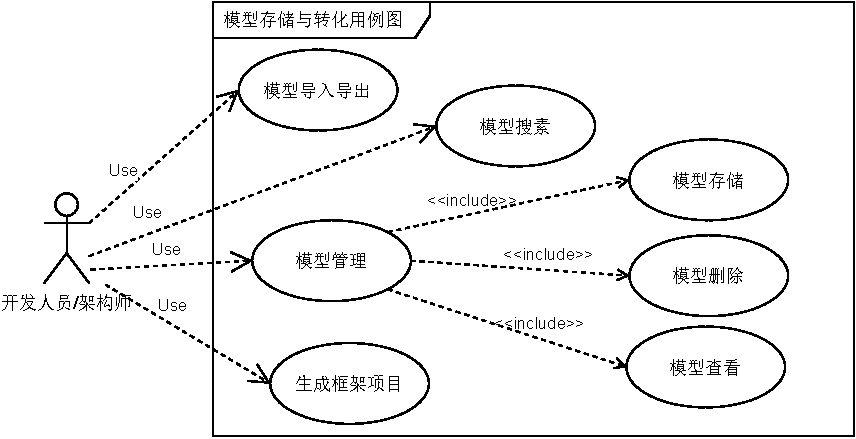
\includegraphics[width=0.8\textwidth]{FIGs/chapter4/us3.pdf} %中括号中的参数是设置图片充满文档的大小,你也可以使用小数来缩小图片的尺寸。
    \caption{模型存储与转化模块用例图} %caption是用来给图片加上图题的
    \label{us3} %这是添加标签,方便在文章中引用图片。
\end{figure}%figure环境

表\ref{usecase3}展示了“模型存储与转化”模块的用例描述,
“模型管理”可以将通过验证的建模结果保存到数据库中,
“模型导入导出”可以将模型以XML、图片等文件格式导出到本地,
也可以导入本地模型文件或搜索数据库中现有模型进行展示和修改,
通过“生成框架项目”可以得到符合领域驱动设计规范的框架项目代码包。

{\footnotesize
    \begin{longtable}[h]{m{80pt}|m{305pt}}
        \caption[模型存储与转化用例表]{模型存储与转化用例表} \label{usecase3} \\
            \hline  
            ID&UC3\\
            \hline
            名称&模型存储与转化\\
            \hline
            描述&将图形化建模结果存储到数据库,或直接以XML、图形等格式导出到本地,
            也可以从本地导入XML模型文件,根据完整的建模结果,自动生成符合领域驱动设计
            结构规范的框架项目代码\\
            \hline
            触发条件&绘图界面点击“导入”、“导出”、“验证”、“保存”或“生成项目”按钮\\
            \hline
            前置条件&建模进行中或已经完成\\
            \hline
            后置条件&无\\
            \hline
            正常流程& (1)进入绘图界面时,可以选择导入本地模型文件或搜索数据库中模型文件进行继续建模;
            \newline (2)模型验证通过后,选择导出建模结果到本地或存储到数据库中;
            \newline (3)点击绘图面板上方“生成项目”按钮可以生成框架项目文件。\\
            \hline
            异常流程&保存建模结果时未填写名称,提示填写\\
            \hline
        \end{longtable} 
}

\textbf{非功能性需求}

“模型存储与转化”模块的非功能性需求主要包括可扩展性、可靠性和性能,
具体需求如下:
        
        \begin{itemize}
            \item 可扩展性:工具采用前后端分离的结构,
            可以对前端或后端组件进行替换或扩展。
            满足存储持久化设施多样性,
            为后续存储更多模型提供保障。
        
            \item 可靠性:工具支持本地文件系统的导入导出,
            不强依赖远程数据库,满足各种网络条件下的建模需求。
           
             \item 性能:对于数据存储和检索使用了ElasticSearch,
             基于倒排索引能达到高效的全文搜索\cite{divya2013elasticsearch}。
             满足搜索模型的即时性,让工具使用速度提升。
        \end{itemize}

\section{工具设计与实现}
\subsection{总体设计}


% 支持建模方法的工具使用流程如下图\ref{toolprocess}所示。
% 开发者使用支持工具开始建模,首先可以选择学习或回顾DDD基本概念知识,
% 为后续建模做理论准备,也可以继续从上一次建模保存的结果开始继续建模;
% 进行可视化建模时,开发者可以随时进行对建模结果的验证,
% 工具将对不符合规范的建模结果给出提示和警告;如果建模结果符合规范和约束,
% 工具将保存建模结果到数据库,通过工具可以将建模结果以XML、图片或Json格式导出;
% 最后,还可以根据建模结果生成框架项目文件。

本工具的架构根据典型的四层架构\cite{王君2007基于}进行设计和划分,
整体架构图如图\ref{overallarchitecture}所示。
第一层表现层负责向用户展示业务流程和数据,包含可视化建模
与验证修改模型等功能;第二层服务层,包含对模型的
存储以及读取、对模型的二次校验和框架项目文件生成功能;
第三层持久层主要保存了业务模型对象的数据,
即对实体、值对象和领域服务等对象数据进行保存;
第四层数据层主要负责建模结果的保存和读取。

\begin{figure}[!htbp] %figure环境,h默认参数是可以浮动,不是固定在当前位置。如果要不浮动,你就可以使用大写float宏包的H参数,固定图片在当前位置,禁止浮动。
    \centering %使图片居中显示
    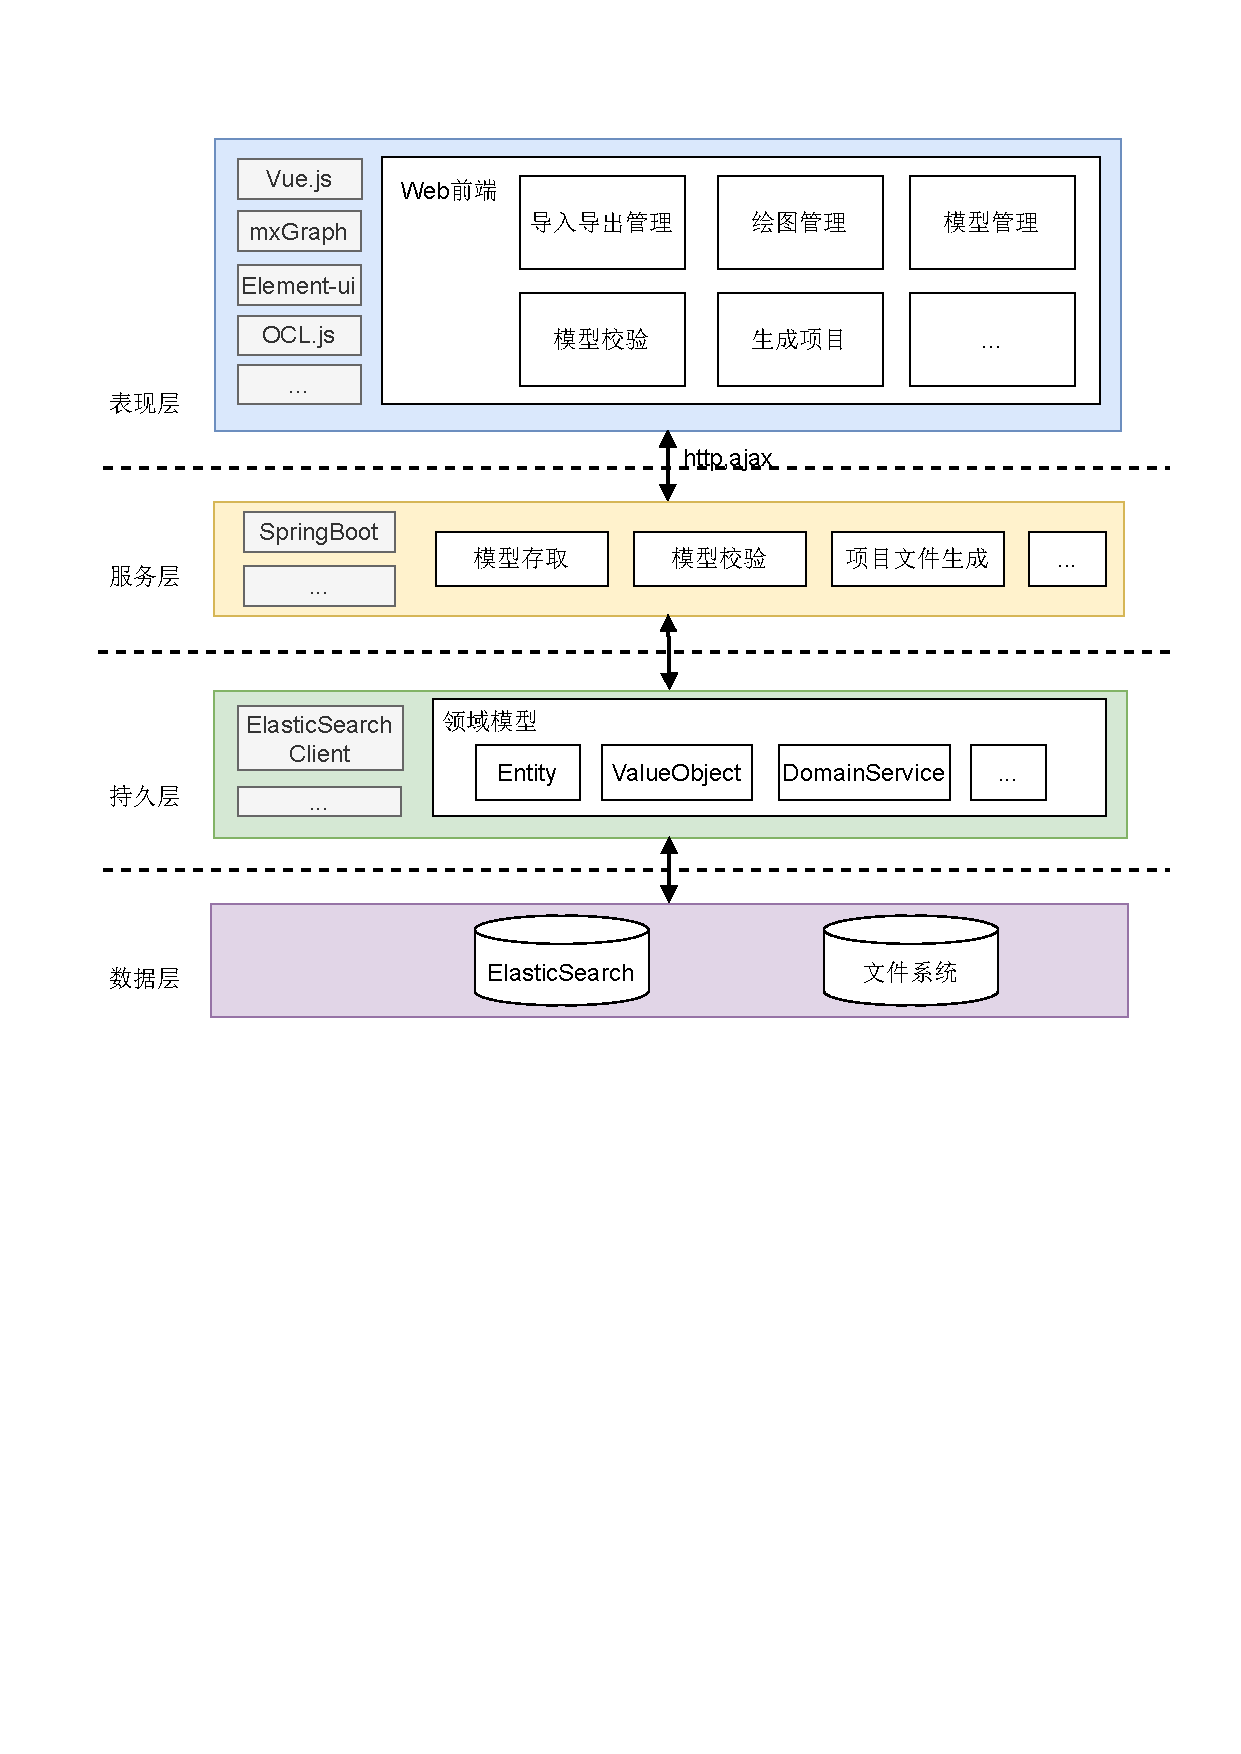
\includegraphics[width=0.8\textwidth]{FIGs/chapter4/overallarchitecture.pdf} %中括号中的参数是设置图片充满文档的大小,你也可以使用小数来缩小图片的尺寸。
    \caption{支持工具整体架构图} %caption是用来给图片加上图题的
    \label{overallarchitecture} %这是添加标签,方便在文章中引用图片。
\end{figure}%figure环境


\begin{itemize}
    \item 表现层:该层为用户提供访问入口,通过该层用户可以直观地使用
    “可视化建模”、”模型校验“等工具核心功能。工具前端采用Vue.js框架
    结合ElementUI组件进行开发,使整个页面整洁美观,交互良好;对于
    图形的拖拽和绘制,采用开源框架mxGraph作为底层支持,mxGraph拥有
    优秀的交互和卓越的性能,已经在许多商业软件中被使用,能有效支持灵活的
    图形编辑;OCL.js主要用来支持模型规范和标准的校验,充当对象约束语言和
    前端JavaScript之间的媒介,可以直接使用JavaScript完成OCL的功能。
    \item 服务层:该层主要提供后端接口服务和对建模逻辑的二次验证。
    后端整体采用Spring Boot框架进行开发,封装抽象了核心的业务逻辑模型(实体、值对象等),
    提供了模型存取与框架项目文件生成的业务逻辑。
    \item 持久层:该层主要充当数据层与服务层间交互的媒介,将业务逻辑模型
    对象转化为底层数据。持久化存储采用ElasticSearch Client与数据层进行
    通信,通过RESTful接口进行写入和读取。
    \item 数据层:该层是底层的存储数据依赖,模型底层存储格式为XML文件,
    文件篇幅较长,但对读写并发要求不高。采用两种数据基础设施进行实现,
    采用ElasticSearch支持大篇幅文档型数据存储,提高模型搜索的检索效率,
    也可根据用户需要直接存储到本地文件系统。
\end{itemize}

建模支持工具DDDD是一个前后端分离的Web应用。前端采用mxGraph结合Vue.js
进行开发实现,后端采用Spring Boot框架,以ElasticSearch作为持久化机制
进行实现,前后端采用RESTful风格进行交互\cite{richardson2008restful}。

由于建模过程的可视化描述和模型校验反馈是工具的核心内容,
负责与用户交互和展示模型的Web前端的架构也有一定复杂度,
故采用如图\ref{frontarchitecture}所描述的整洁架构\cite{martin2018clean}对前端进行划分。
整洁架构是一种与数据库、客户端接口以及框架都无关的架构,
可以用来构建复杂的前端项目,将业务逻辑抽离,但又不依赖后端,保证项目的可扩展性。
本工具使用整洁架构将前端划分为三层,包括表现层、领域层和数据层。
表现层包含绘图、校验、导入导出以及菜单等与用户交互的模块;
领域层包含展示模型和校验反馈的底层业务逻辑,如拖拽绘制、
校验模型、导入导出模型、画布管理、路由管理以及生成项目等功能;
数据层包含调用后端API连接的远程数据源和本地数据源,
负责存储和获取模型。

\begin{figure}[htb] %figure环境,h默认参数是可以浮动,不是固定在当前位置。如果要不浮动,你就可以使用大写float宏包的H参数,固定图片在当前位置,禁止浮动。
    \centering %使图片居中显示
    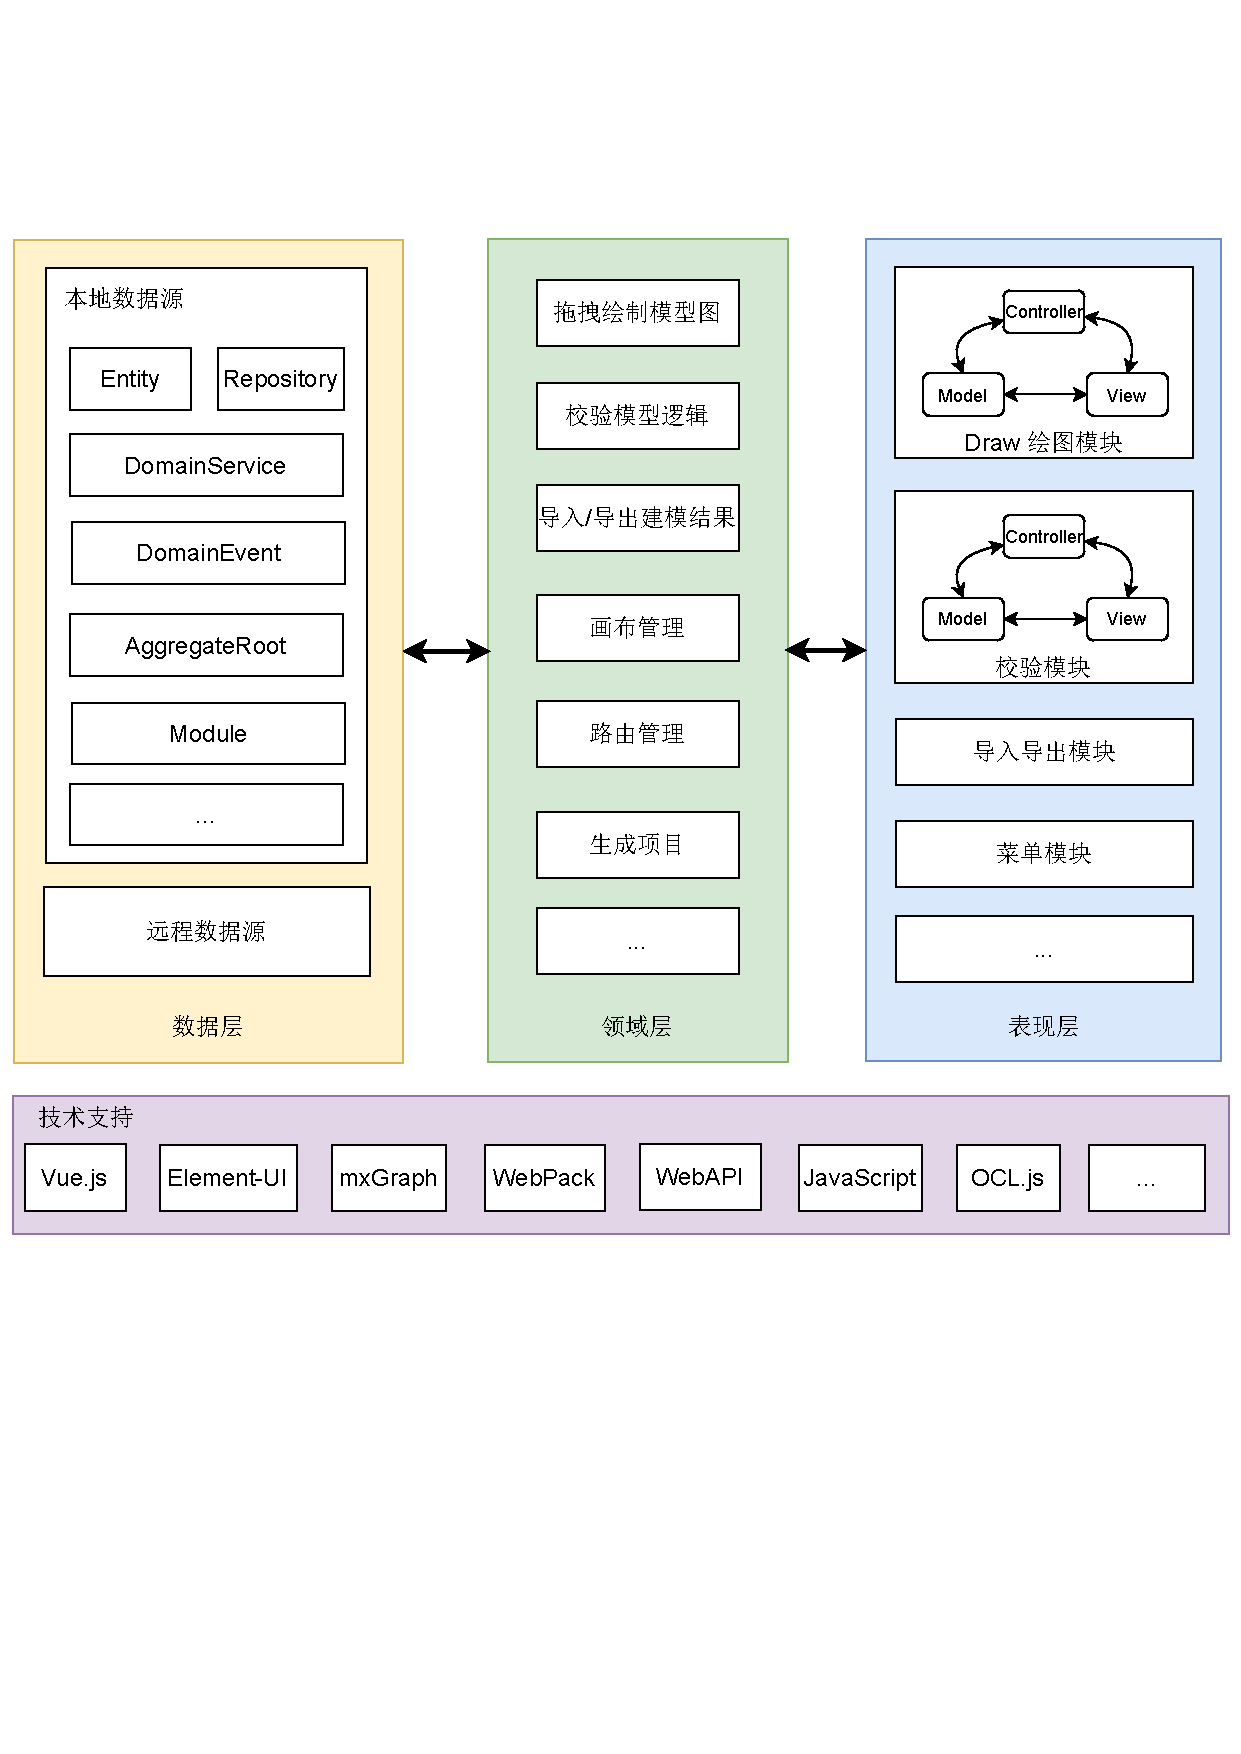
\includegraphics[width=0.8\textwidth]{FIGs/chapter4/frontarchitecture.pdf} %中括号中的参数是设置图片充满文档的大小,你也可以使用小数来缩小图片的尺寸。
    \caption{支持工具前端整洁架构图} %caption是用来给图片加上图题的
    \label{frontarchitecture} %这是添加标签,方便在文章中引用图片。
\end{figure}%figure环境


\subsection{可视化建模模块详细设计与实现}

本小节将介绍“可视化建模”模块的详细设计与实现。详细设计部分,
通过类图展现“可视化建模”模块的静态详细设计,
通过顺序图展现“可视化建模”模块的动态业务流程详细设计。
实现部分,通过部分核心功能的实现代码来进行展现。
“可视化建模”模块具体的设计如下:

\textbf{可视化建模类图}

“可视化建模”模块类图如图\ref{classDrawVisualization}所示。
本工具提供对建模过程可视化的支持,主要由Canvas类对mxGraph中
封装好的画图工具类接口进行调用,并确保工具类是单例的,
Canvas类还负责工具运行时对画布的初始化,保证画图时的线条、箭头和颜色
符合预期,最后,还包含绘制新图形时的判断逻辑。Toolbar类主要
提供了建模时对模式的选择支持,可以直接从中点击拖动实现选择战术模式。
Menu类包含了对画布操作的一系列接口。
Container类负责统一管理Toolbar、Canvas和Menu类,并收集反馈信息与用户进行交互。

\begin{figure}[!htbp] %figure环境,h默认参数是可以浮动,不是固定在当前位置。如果要不浮动,你就可以使用大写float宏包的H参数,固定图片在当前位置,禁止浮动。
    \centering %使图片居中显示
    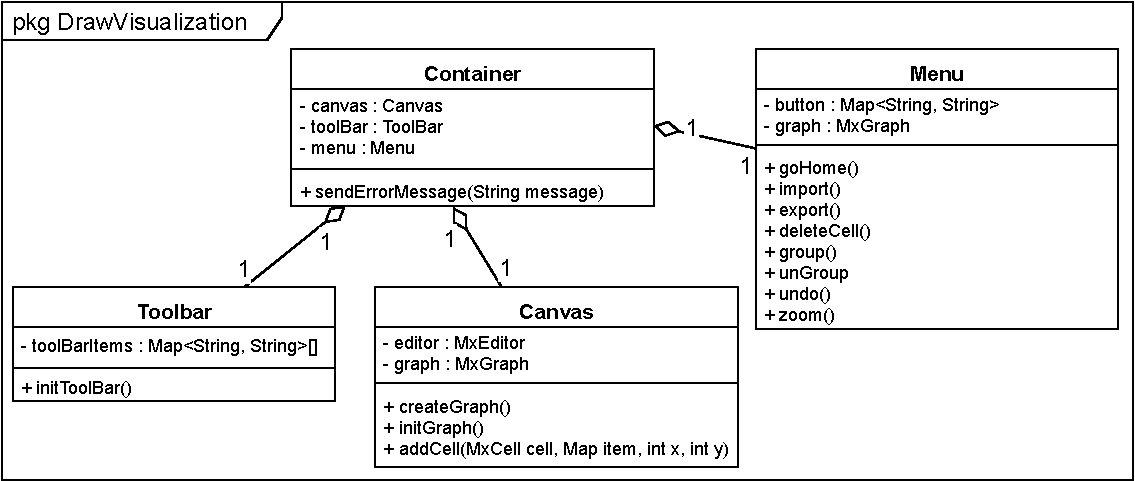
\includegraphics[width=0.8\textwidth]{FIGs/chapter4/classDrawVisualization.pdf} %中括号中的参数是设置图片充满文档的大小,你也可以使用小数来缩小图片的尺寸。
    \caption{可视化建模模块类图} %caption是用来给图片加上图题的
    \label{classDrawVisualization} %这是添加标签,方便在文章中引用图片。
\end{figure}%figure环境

\textbf{可视化建模顺序图}

“可视化建模”模块的示例过程如图\ref{sdDrawVisualization}所示。
首先开发人员或架构师通过使用Container类初始化画布、工具栏等可视化建模必要元素,
通过Toolbar类实现拖拽图形化模式对象,并在合适的位置由Canvas类绘制,
在建模过程中,通过菜单可以实现撤销、重做、组合、删除、缩放画布等一系列操作,
辅助完成建模过程,在建模过程中画布会实时反馈信息给用户。

\begin{figure}[!htbp] %figure环境,h默认参数是可以浮动,不是固定在当前位置。如果要不浮动,你就可以使用大写float宏包的H参数,固定图片在当前位置,禁止浮动。
    \centering %使图片居中显示
    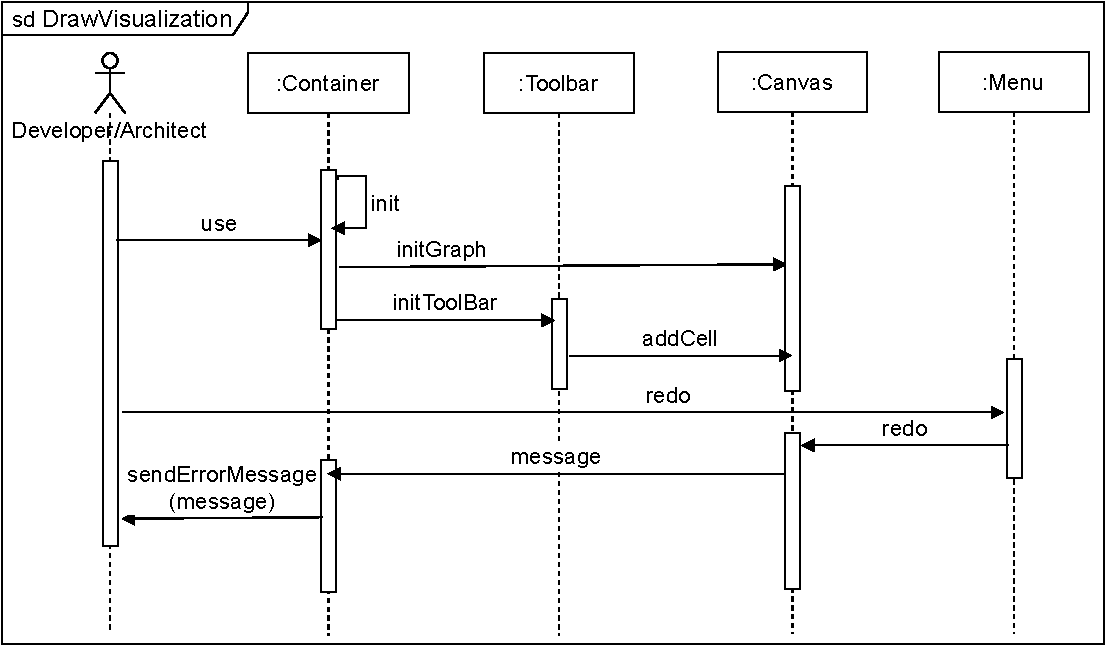
\includegraphics[width=0.8\textwidth]{FIGs/chapter4/sdDrawVisualization.pdf} %中括号中的参数是设置图片充满文档的大小,你也可以使用小数来缩小图片的尺寸。
    \caption{可视化建模模块顺序图} %caption是用来给图片加上图题的
    \label{sdDrawVisualization} %这是添加标签,方便在文章中引用图片。
\end{figure}%figure环境

\newpage
\textbf{可视化建模实现代码}

如图\ref{initToolbar}所示为“可视化建模”核心功能工具栏的初始化代码。
代码描述了获取图形对象数组、拖动图形、绘制图形的逻辑。

\begin{figure}[!htbp] %figure环境,h默认参数是可以浮动,不是固定在当前位置。如果要不浮动,你就可以使用大写float宏包的H参数,固定图片在当前位置,禁止浮动。
    \centering %使图片居中显示
    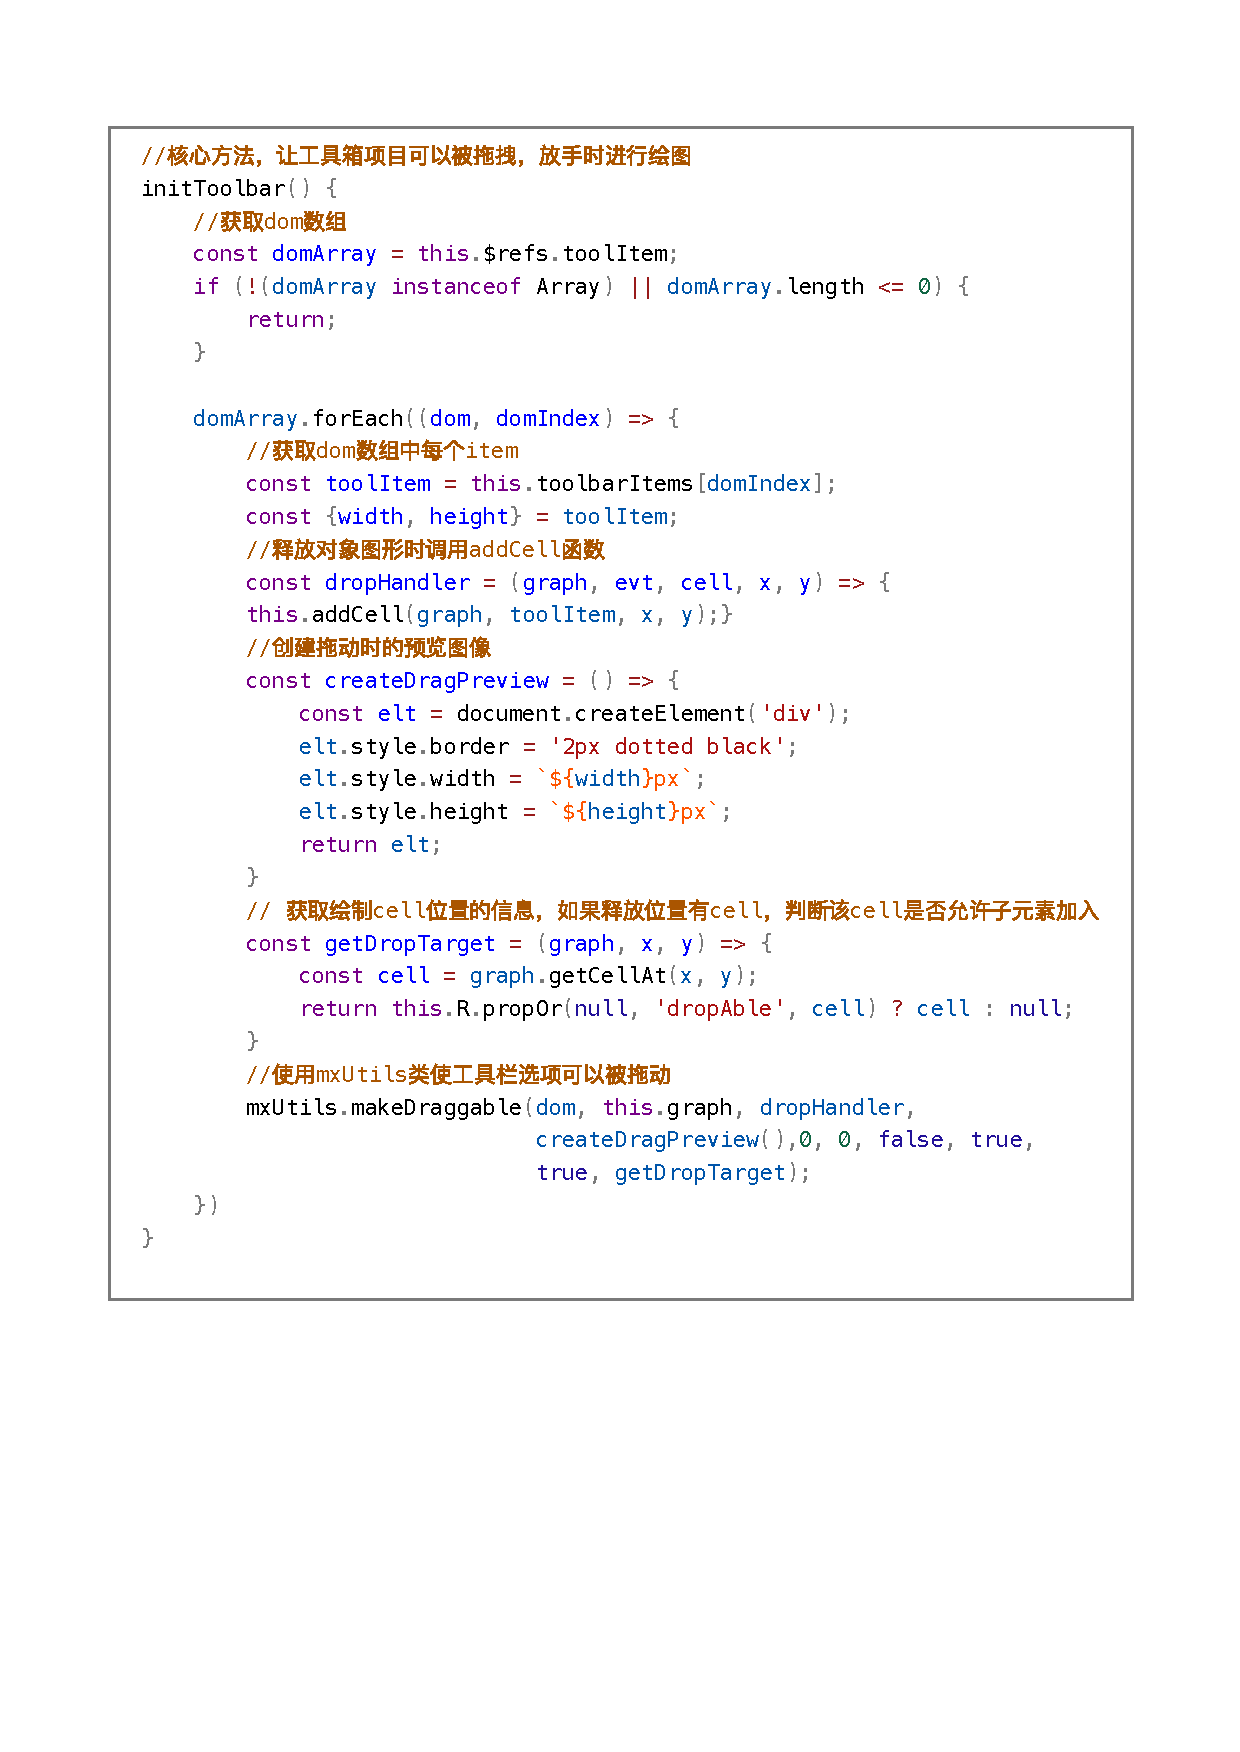
\includegraphics[width=0.8\textwidth]{FIGs/chapter4/initToolbar.pdf} %中括号中的参数是设置图片充满文档的大小,你也可以使用小数来缩小图片的尺寸。
    \caption{初始化ToolBar代码} %caption是用来给图片加上图题的
    \label{initToolbar} %这是添加标签,方便在文章中引用图片。
\end{figure}%figure环境 

\subsection{模型校验模块详细设计与实现}

本小节将介绍“模型校验”模块的详细设计与实现。详细设计部分,
通过类图展现“模型校验”模块中各战术模式的静态详细设计;
实现部分,
通过校验算法展现“模型校验”模块的验证逻辑的设计,
通过部分实现代码展示具体实现。
“模型校验”模块具体的设计如下:

\newpage
\textbf{模型校验类图}

“模型校验”模块类图如图\ref{classValidation}所示。
本工具提供对建模结果的校验,战术模式统一继承自Pattern类,
Pattern类描述了模式的名称、类型、连接输入以及连接输出,
并在validation方法中调用OCLEngine对象实例完成对象约束语言的验证。
PatternData用来记录所有Pattern子类实例的数据细节,
辅助校验过程。


\begin{figure}[!htbp] %figure环境,h默认参数是可以浮动,不是固定在当前位置。如果要不浮动,你就可以使用大写float宏包的H参数,固定图片在当前位置,禁止浮动。
    \centering %使图片居中显示
    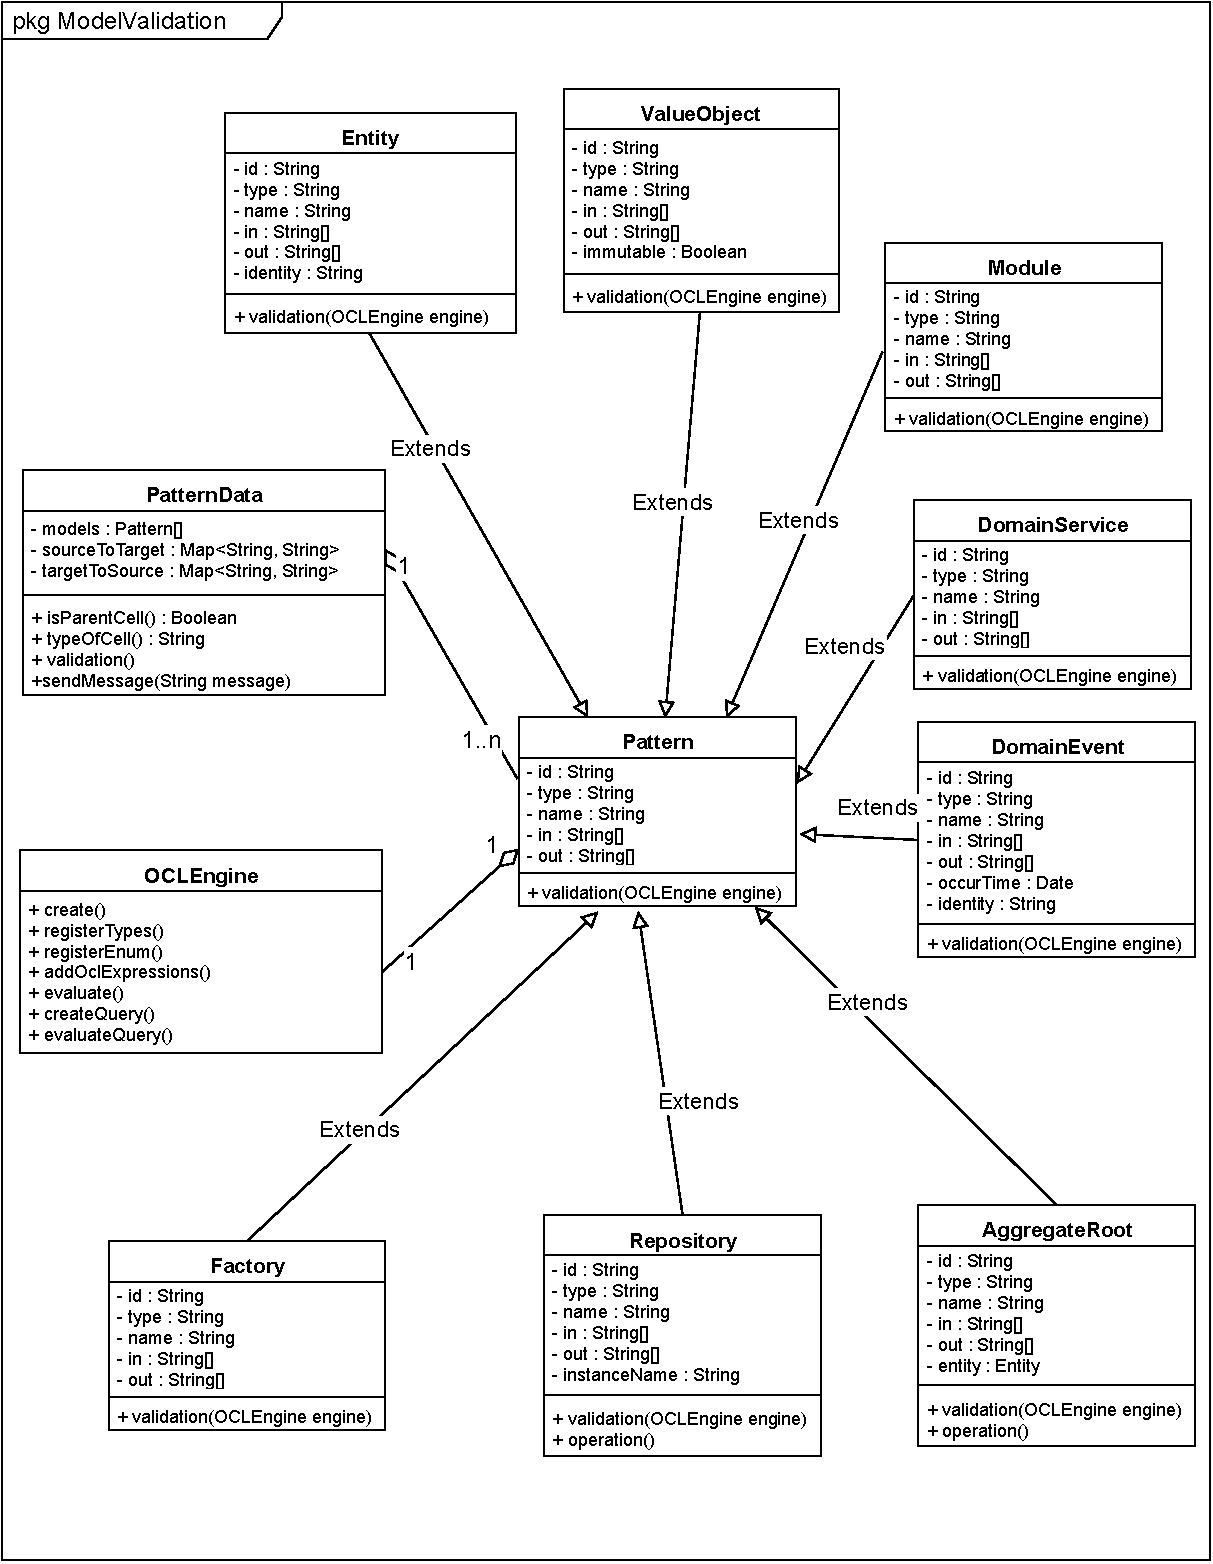
\includegraphics[width=0.8\textwidth]{FIGs/chapter4/classValidation.pdf} %中括号中的参数是设置图片充满文档的大小,你也可以使用小数来缩小图片的尺寸。
    \caption{模型校验模块类图} %caption是用来给图片加上图题的
    \label{classValidation} %这是添加标签,方便在文章中引用图片。
\end{figure}%figure环境

\textbf{模型校验算法}

“模型校验”功能的具体实现逻辑如算法\ref{algorithm1}所示。该算法首先通过遍历所有图形化对象节点,
建立两种连接关系双向映射,第一种描述源对象到目标对象映射关系,第二种描述目标对象到源对象映射关系;
然后进行第二次遍历,首先判断该对象节点是否为顶级节点,只有顶级节点才作为战术模式元素,
如果为顶级节点,则调用PatternData类中的validation函数进行模式属性以及OCL约束验证,
验证通过将该对象以具体模式(实体、值对象等)添加到patternData的models数据结构中,若验证失败,
将布尔型成功标识变量标记为否,并退出循环体。无论验证是否通过,都将非顶级节点的子节点跳过,节省验证时间;
如果不是顶级节点,则继续执行循环体;最终返回验证结果及具体建模结果。


\begin{algorithm}[!htbp]
    \floatname{algorithm}{\footnotesize 算法}
    \caption{\footnotesize 模型校验算法}
    \label{algorithm1}
    {\footnotesize
    \begin{algorithmic}
        \renewcommand{\algorithmicrequire}{ \textbf{Input:}}
        \REQUIRE  
        mxCells:HTMLCollectionOf<Element>

        \REQUIRE
        patterns:PatternData

        \renewcommand{\algorithmicensure}{\textbf{Output:}}
        \ENSURE
        models:Map<String, Pattern>

        \STATE{Boolean success = true;}
        \FOR{mxCell in mxCells}

        \STATE{patterns.setSourceToTarget(mxCell.getId, mxCell.getTarget);}

        \STATE{patterns.setTargetToSource(mxCell.getSource, mxCell.getId);}
        
        \ENDFOR

        \FOR{mxCell in mxCells}
            \IF{patterns.isParentCell(mxCell)}
                \IF{patterns.validation(mxCell)}
                    \STATE{newPattern = new Pattern(mxCell);}
                    \STATE{patterns.models.add(mxCell.getId, newPattern);}
                \ELSE
                    \STATE{success = false;}
                    \STATE{break;}
                \ENDIF
            \STATE{skip loopStep;}
            \ELSE
            \STATE{continue loop;}
            \ENDIF
        \ENDFOR
          
        \IF{success}

            \STATE{sendSuccessMessage();}

            \STATE{return patterns.models;}

        \ELSE
            \STATE{sendErrorMessage();}
        
        \ENDIF
        
    \end{algorithmic}
    }
\end{algorithm}


\textbf{模型校验实现代码}

如图\ref{validationCode}所示是“模型校验”功能部分实现代码。主要描述validation方法中
对DomainService对象的验证过程,包括从图形化对象转化为抽象模式类的过程以及
对象约束语言验证与属性验证。

\begin{figure}[!htbp] %figure环境,h默认参数是可以浮动,不是固定在当前位置。如果要不浮动,你就可以使用大写float宏包的H参数,固定图片在当前位置,禁止浮动。
    \centering %使图片居中显示
    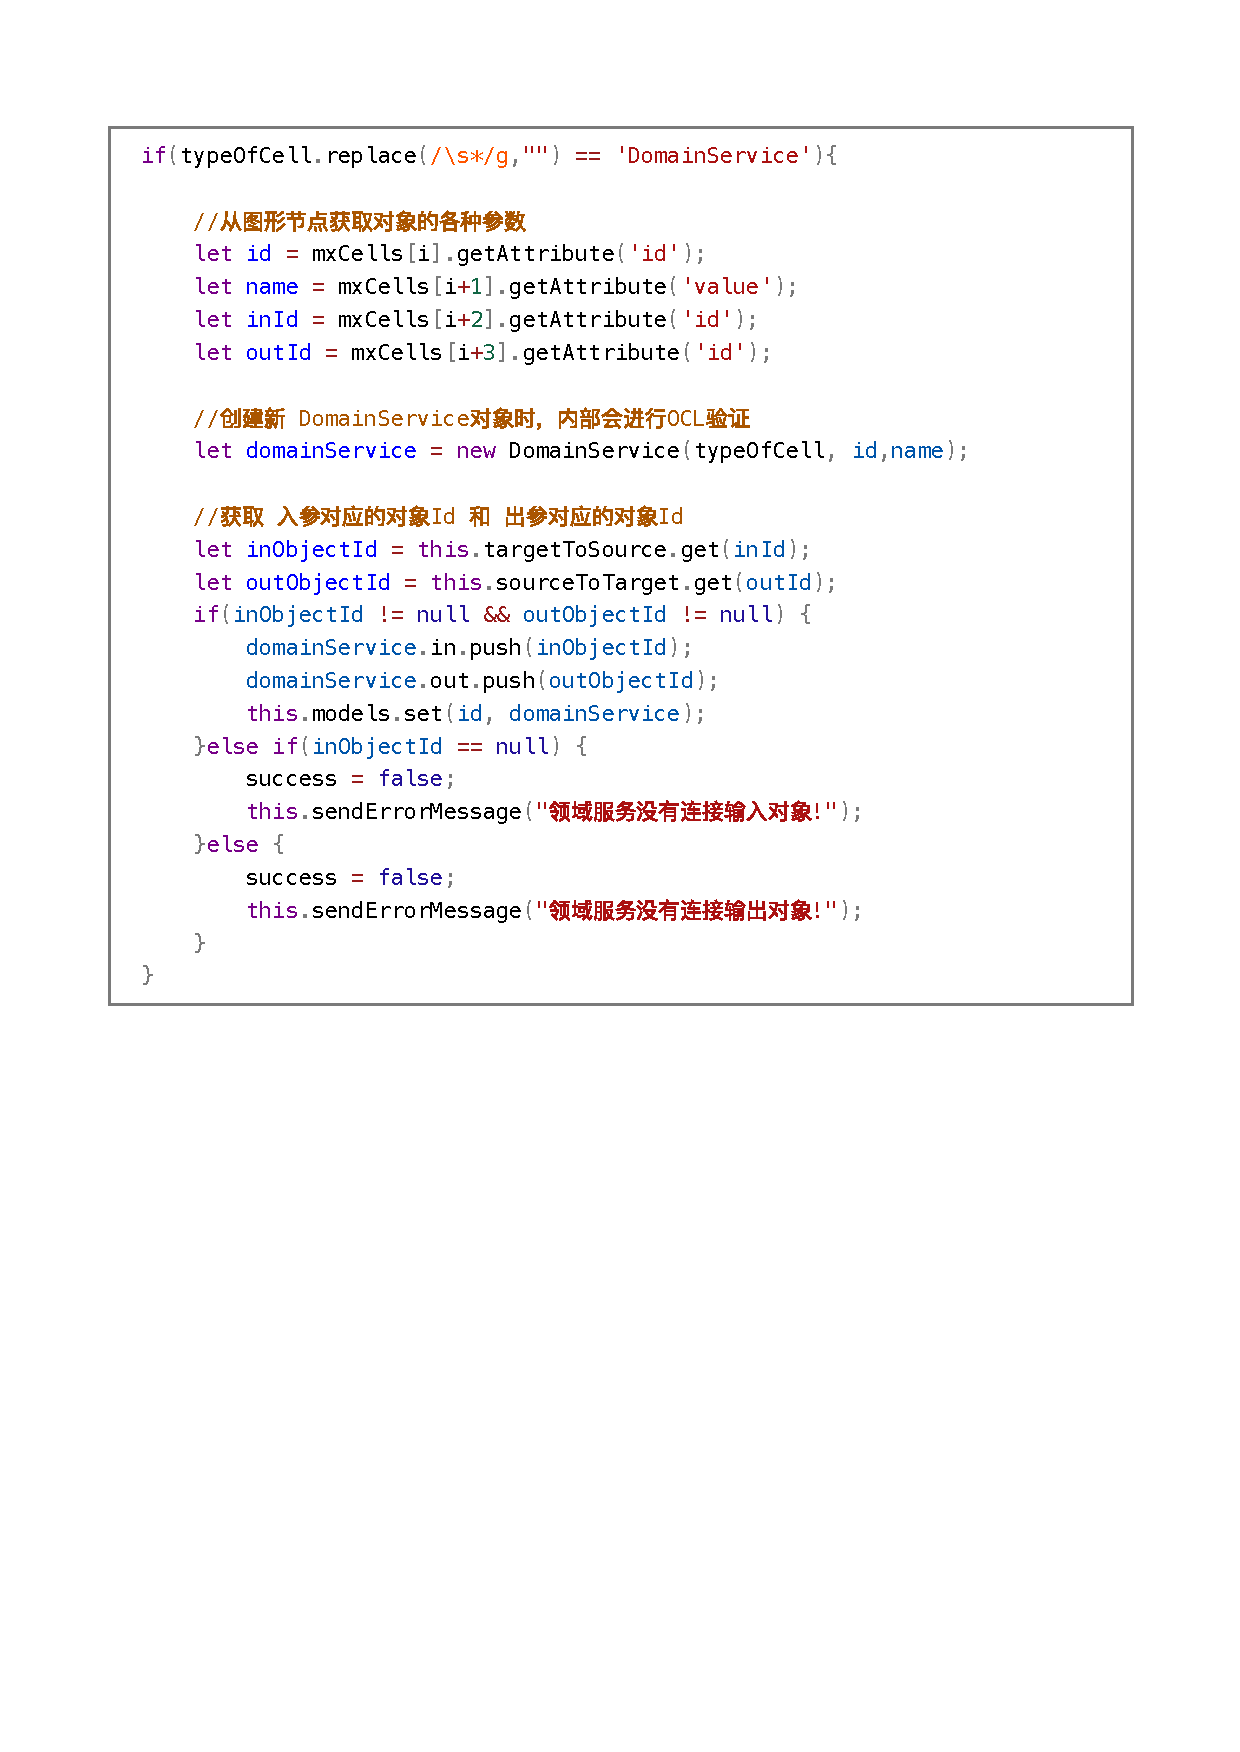
\includegraphics[width=0.8\textwidth]{FIGs/chapter4/validation.pdf} %中括号中的参数是设置图片充满文档的大小,你也可以使用小数来缩小图片的尺寸。
    \caption{模型校验部分实现代码} %caption是用来给图片加上图题的
    \label{validationCode} %这是添加标签,方便在文章中引用图片。
\end{figure}%figure环境


\subsection{模型存储与转化详细设计与实现}

本小节将介绍“模型存储与转化”模块的详细设计与实现。详细设计部分,
通过类图展现“模型存储与转化”模块的静态详细设计,
通过顺序图展现“模型存储与转化”模块的动态业务流程详细设计。
实现部分,通过部分核心功能实现代码进行展现。
“模型存储与转化”模块具体的设计如下:

\textbf{模型存储与转化类图}

“模型存储与转化”模块的类图如图\ref{classModelStorage}所示。
本工具提供对建模结果的存储与转化,由File类负责收集和组织图形化模式
的具体信息,可以直接在浏览器客户端导出建模结果的XML格式文件和图像格式文件,
也可以导入模型的XML文件,直接将模型绘制在画布上继续进行编辑;
当与后端进行通信时,会将模型信息抽象为Model类,由ModelRepository负责
模型的存储、修改、删除以及检索,
使用ElasticSearch提供的客户端进行持久化支持,
可以极大提升检索模型文件的效率。

\begin{figure}[!htbp] %figure环境,h默认参数是可以浮动,不是固定在当前位置。如果要不浮动,你就可以使用大写float宏包的H参数,固定图片在当前位置,禁止浮动。
    \centering %使图片居中显示
    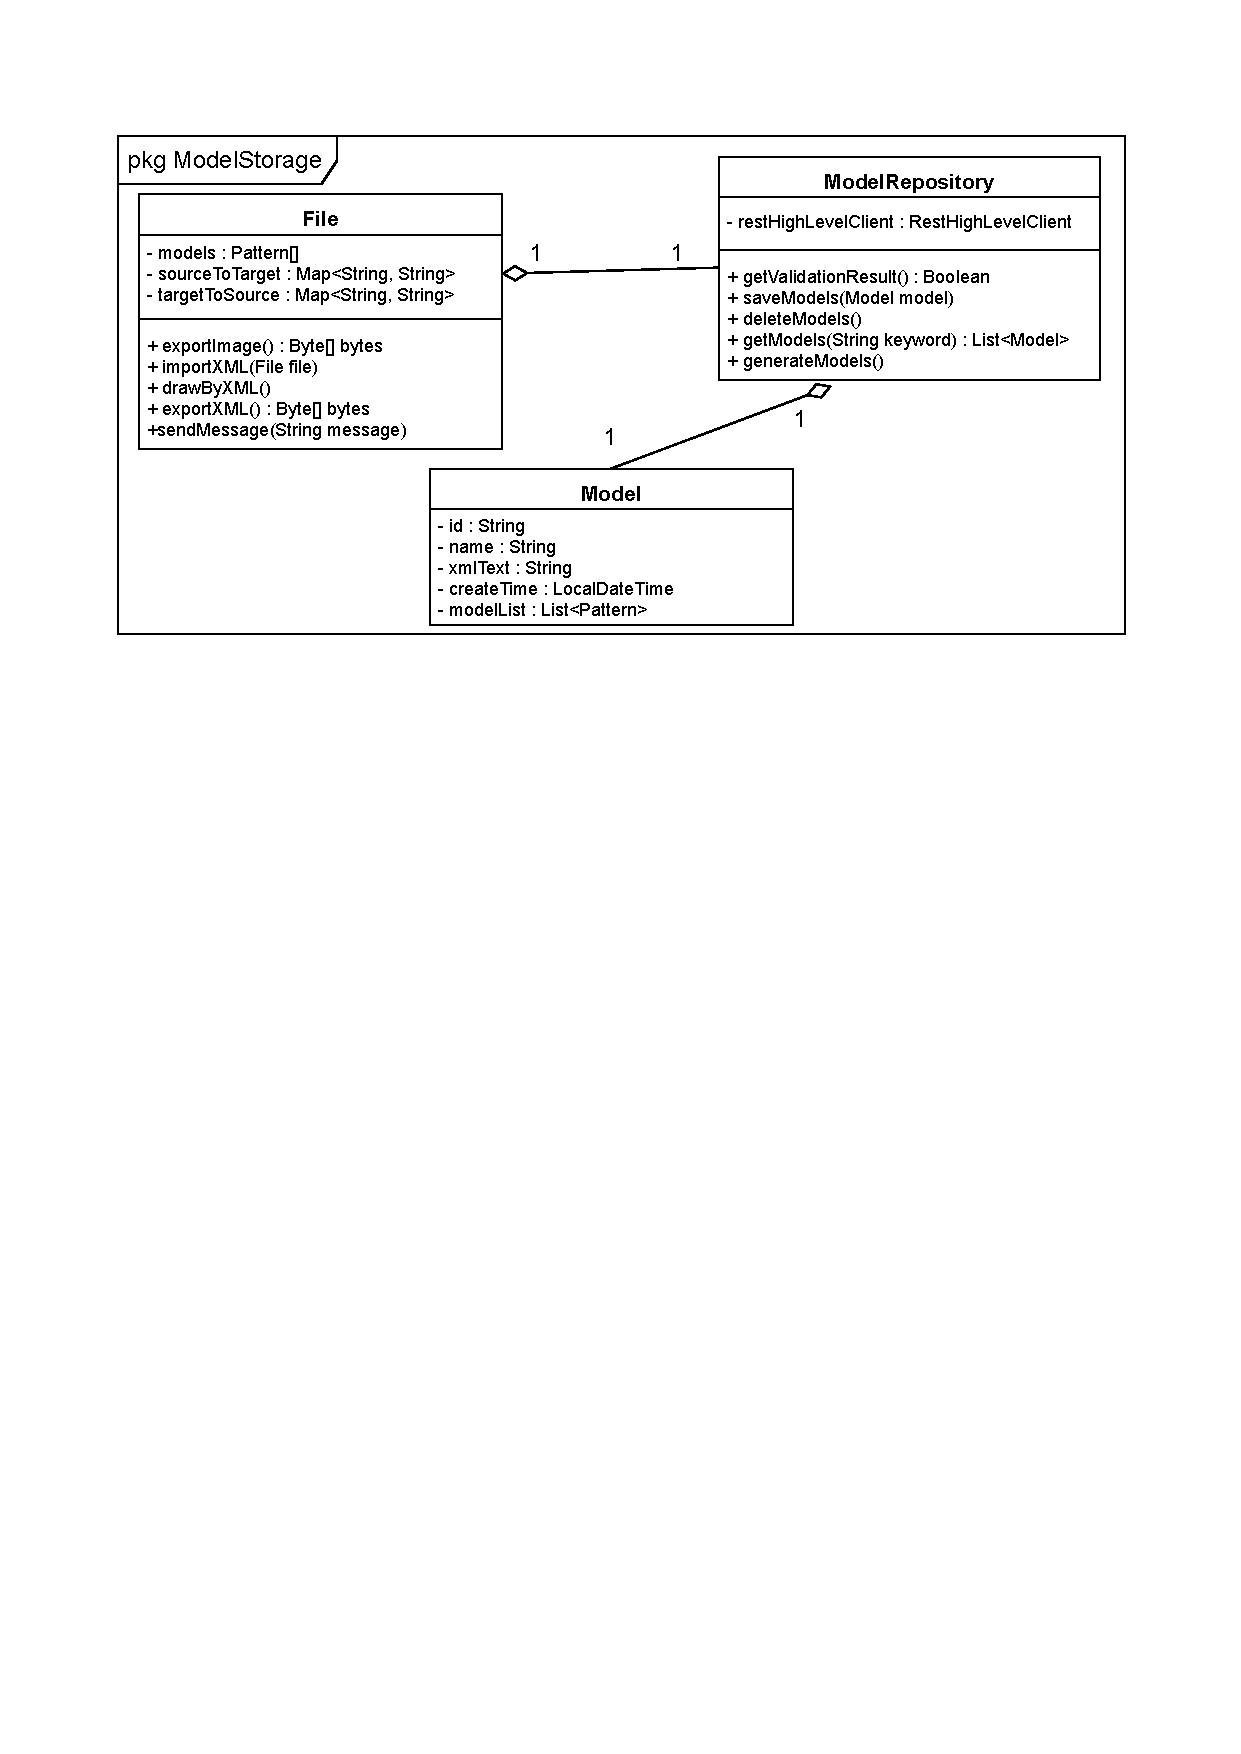
\includegraphics[width=0.8\textwidth]{FIGs/chapter4/classModelStorage1.pdf} %中括号中的参数是设置图片充满文档的大小,你也可以使用小数来缩小图片的尺寸。
    \caption{模型存储与转化类图} %caption是用来给图片加上图题的
    \label{classModelStorage} %这是添加标签,方便在文章中引用图片。
\end{figure}%figure环境

\newpage
\textbf{模型存储与转化顺序图}

“模型存储与转化”功能的示例过程如图\ref{sdModelStorage}所示。
开发人员或架构师使用浏览器客户端将XML模型文件导入画布,可以直接进行编辑,
编辑完成后,可以选择导出为XML文件或图像格式,
也可以将模型存储到数据库中并生成符合领域驱动设计规范的框架项目。

\begin{figure}[!htbp] %figure环境,h默认参数是可以浮动,不是固定在当前位置。如果要不浮动,你就可以使用大写float宏包的H参数,固定图片在当前位置,禁止浮动。
    \centering %使图片居中显示
    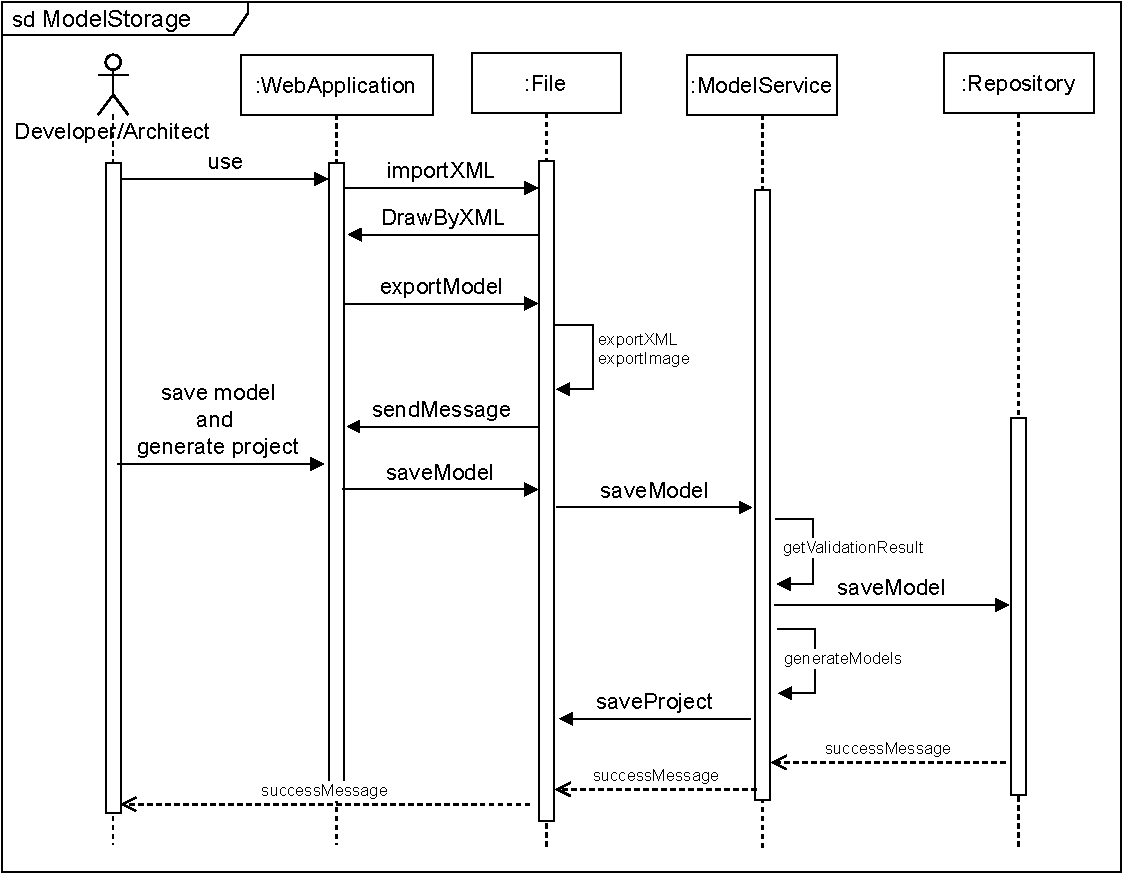
\includegraphics[width=0.8\textwidth]{FIGs/chapter4/sdModelStorage.pdf} %中括号中的参数是设置图片充满文档的大小,你也可以使用小数来缩小图片的尺寸。
    \caption{模型存储与转化顺序图} %caption是用来给图片加上图题的
    \label{sdModelStorage} %这是添加标签,方便在文章中引用图片。
\end{figure}%figure环境

\newpage
\textbf{模型存储部分实现代码}

如图\ref{saveModelcode}所示是“模型存储”部分实现代码。
主要描述将模型存储进ElasticSearch中的过程,
包括对模型对象的构建、存储格式的转化、发起存储请求与接收响应。


\begin{figure}[!htbp] %figure环境,h默认参数是可以浮动,不是固定在当前位置。如果要不浮动,你就可以使用大写float宏包的H参数,固定图片在当前位置,禁止浮动。
    \centering %使图片居中显示
    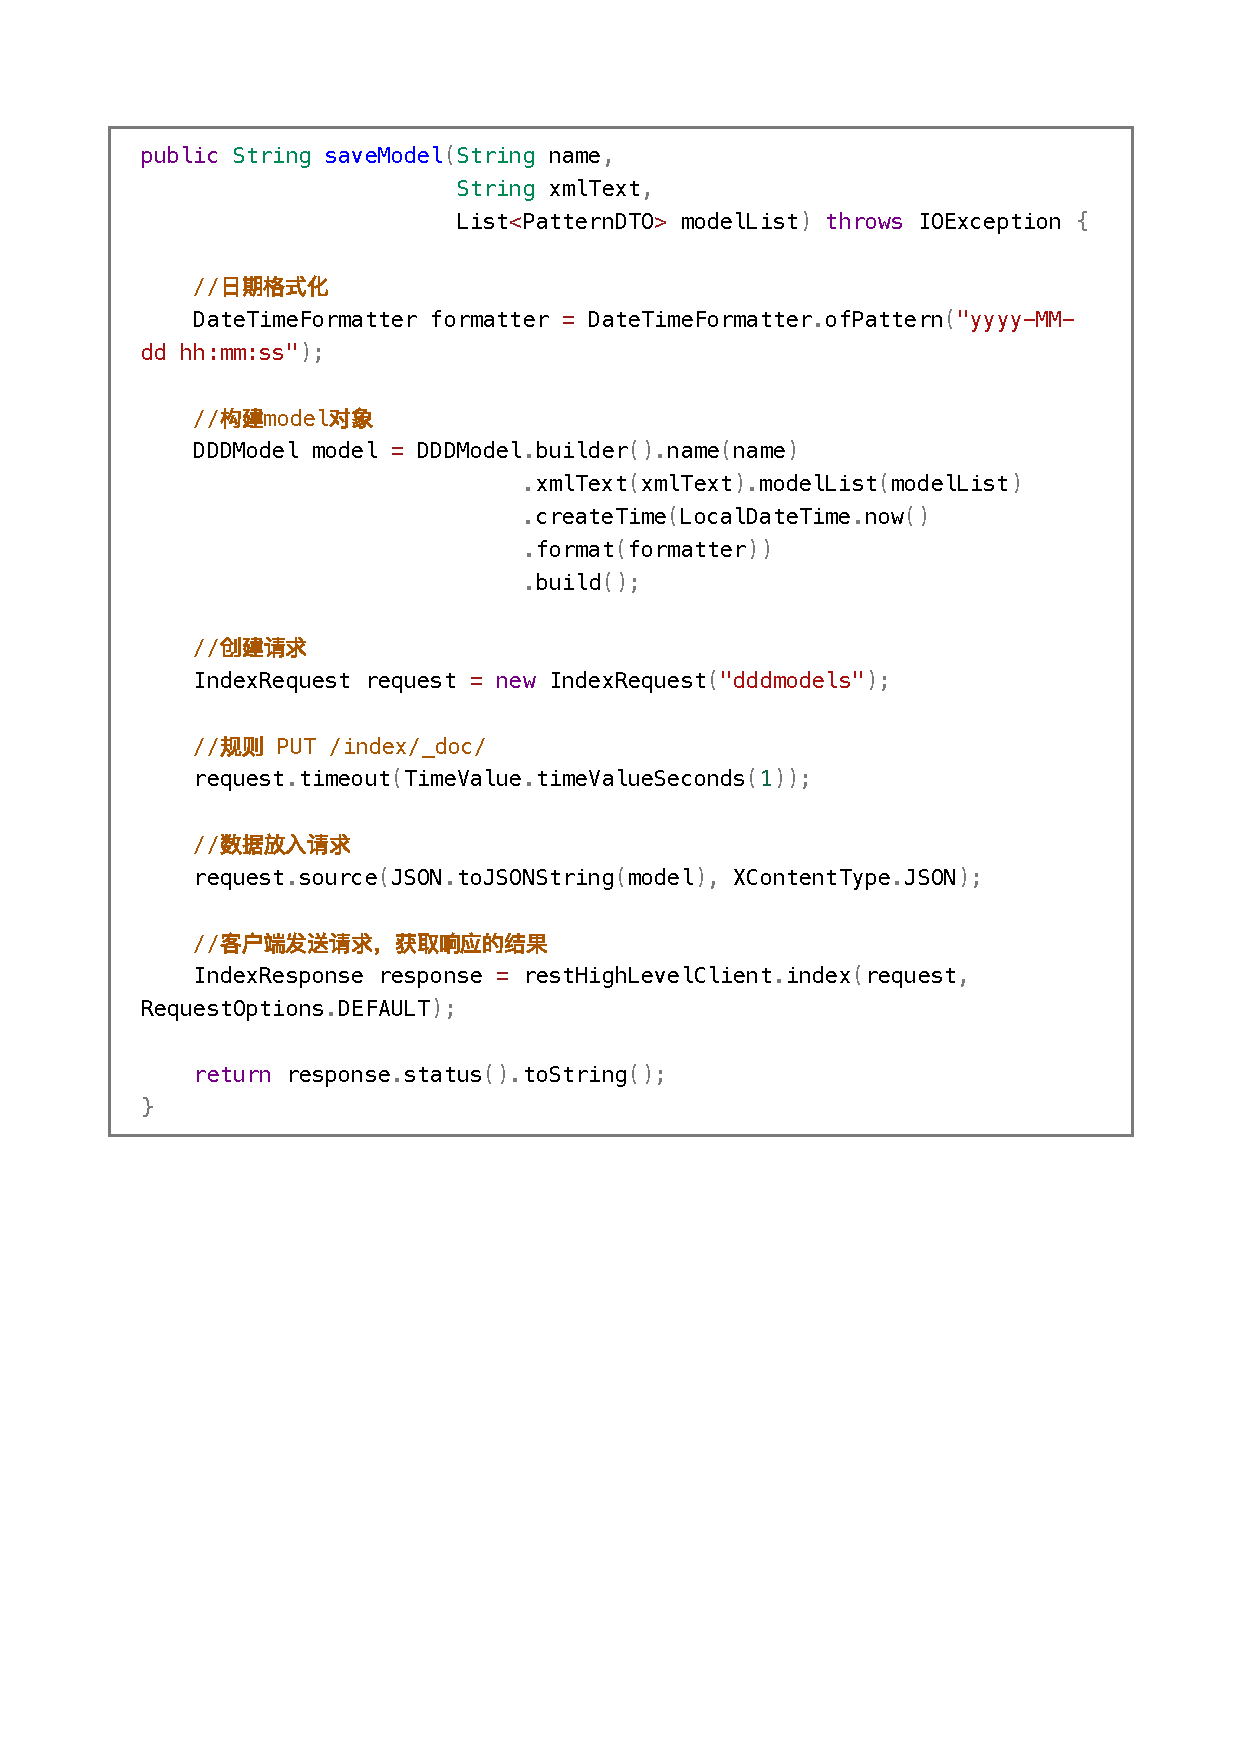
\includegraphics[width=0.8\textwidth]{FIGs/chapter4/saveModelcode.pdf} %中括号中的参数是设置图片充满文档的大小,你也可以使用小数来缩小图片的尺寸。
    \caption{模型存储部分实现代码} %caption是用来给图片加上图题的
    \label{saveModelcode} %这是添加标签,方便在文章中引用图片。
\end{figure}%figure环境

\section{本章小结}

本章介绍了建模支持工具的设计与实现。首先通过对建模场景中的用例分析,
获取具体需求,包括“可视化建模”、“模型校验”以及“模型存储与转化”三个主要模块。
然后对工具进行了功能性与非功能性需求的分析与展示,通过需求对工具进行总体设计
与详细设计。最后通过各模块功能类图、顺序图、功能算法逻辑和实现代码来展示工具的具体实现过程。



\chapter{测试与评估}

本章将介绍面向Hyperledger Fabric的区块链云化框架的测试与评估工作。首先, 本章以典型案例以及SAAM方法对原型工具基本能力自证; 其次, 采用五层成熟度模型进行成熟度衡量; 最后, 与官方工具Cello\footnotemark[1]\footnotetext[1]{\href{https://github.com/hyperledger/cello}{Hyperledger Cello}}进行对比评估。



\section{测试环境}

如图\ref{assessment}所示, 本文从三个方面对本文提出的区块链云化框架与工具进行综合评估。首先是基本能力自证, 本文以典型案例研究的方式证明原型工具的功能完备性以及智能合约微服务改造的可行性, 结合软件体系结构评估方法Software Architecture Analysis Method(简称SAAM)验证区块链云化节点的质量属性; 其次是成熟度衡量, 本文以定性研究\cite{tashakkori1998mixed}的方式结合Operator五层成熟度模型对原型工具进行成熟度能力的评估; 最后是工具的对比分析, 本文将原型工具与Cello进行定量对比, 评估原型工具的网络节点部署时间以及链码交付效率。

\begin{figure}[h] %figure环境,h默认参数是可以浮动,不是固定在当前位置。如果要不浮动,你就可以使用大写float宏包的H参数,固定图片在当前位置,禁止浮动。
    \centering %使图片居中显示
    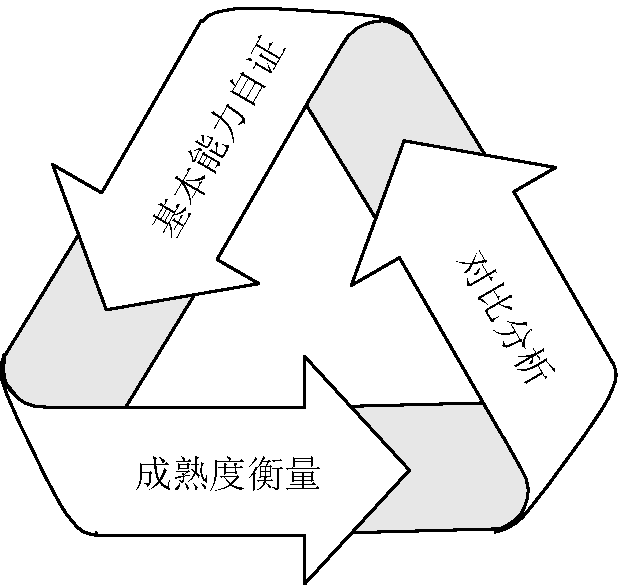
\includegraphics[width=0.4\textwidth]{FIGs/chapter6/assessment.pdf} %中括号中的参数是设置图片充满文档的大小,你也可以使用小数来缩小图片的尺寸。
    \caption{评估体系} %caption是用来给图片加上图题的
    \label{assessment} %这是添加标签,方便在文章中引用图片。
\end{figure}%figure环境

由于在本机环境下搭建Cello会出现诸多问题, 如文件挂载权限、编译等, 所以本文准备了两套测试环境。本文首先在本地环境进行功能方面的测试, 本地机器为MacBook Pro, 并采用Docker for Desktop搭建的单节点Kubernetes充当集群环境; 其次, 在第\ref{section: tool_comparison}节中, 为顺利运行对比工具Cello, 本文利用云主机Ubuntu 18.04搭建Minikube充当集群环境。上述两种环境具体配置如表\ref{computer}所示。

{\footnotesize
\begin{longtable}[h]{m{40pt} m{100pt} m{100pt}}
    \caption[配置详情]{配置详情} \label{computer} \\
        \toprule    
        \textbf{环境} & \textbf{配置项目} & \textbf{配置详情} \\
        \hline
        \multirow{2}*{\parbox[c]{40pt}{本机环境}}    
        & Docker for Desktop&Version 4.7.0\\     
        & Kubernetes&v1.22.5\\
        \hline
        \multirow{3}*{\parbox[c]{40pt}{云主机}} 
        & Docker & Community 20.10.13 \\
        & minikube & v1.25.2 \\
        & Kubernetes & v1.23.3 \\
        \bottomrule 
    \end{longtable} 
}


\section{基本能力自证}\label{section: tool_test}

\subsection{案例研究}

本小节主要以案例研究的方式对原型工具进行功能性测试。如图\ref{fabric_net}所示, 本节将以搭建最经典、简单的HF网络案例的方式针对\ref{section: requirement}节的用例进行完整的功能测试。测试重点针对于Ca、Peer、Orderer启动、创建通道、部署链码、调用的全部过程,验证HF网络启动及链码部署的正确性。

\begin{figure}[h] %figure环境,h默认参数是可以浮动,不是固定在当前位置。如果要不浮动,你就可以使用大写float宏包的H参数,固定图片在当前位置,禁止浮动。
    \centering %使图片居中显示
    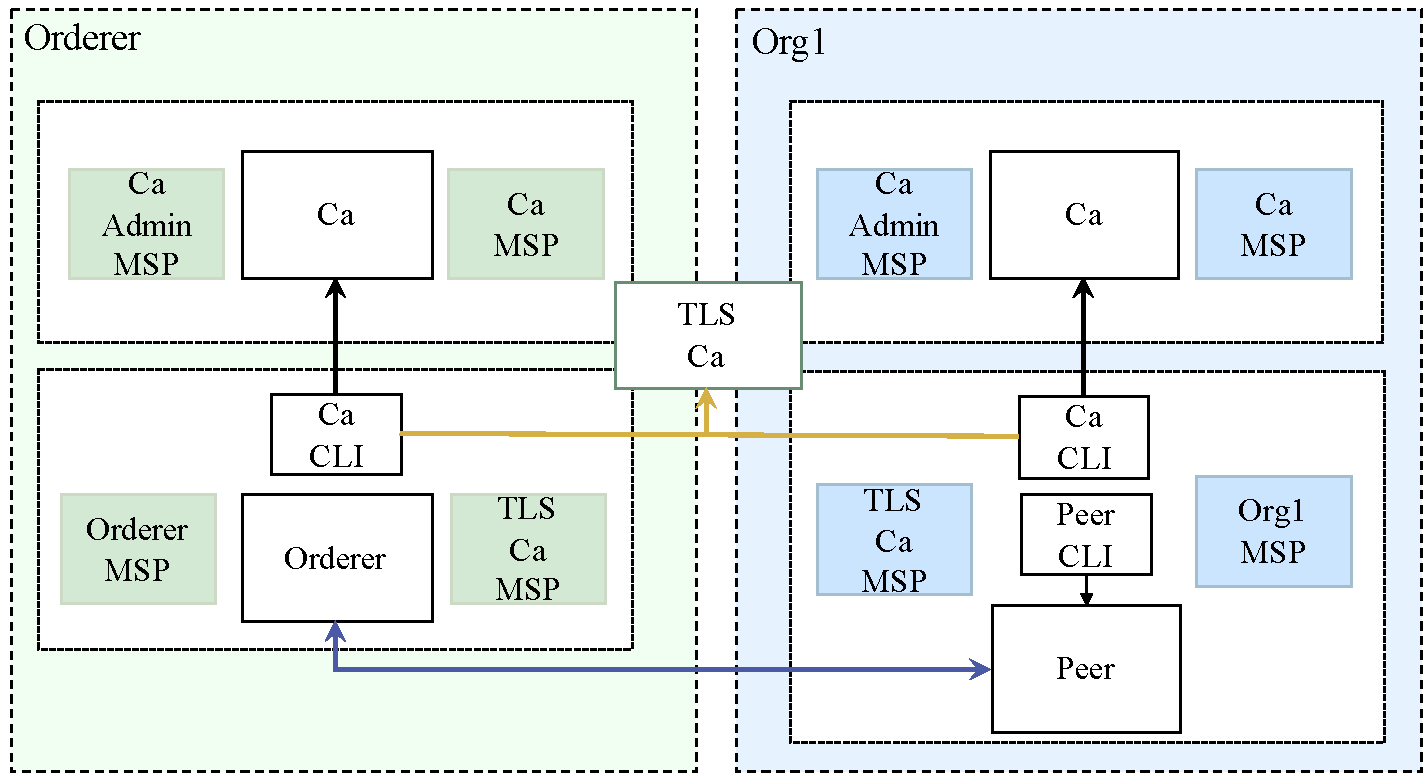
\includegraphics[width=1.0\textwidth]{FIGs/chapter6/fabric_net.pdf} %中括号中的参数是设置图片充满文档的大小,你也可以使用小数来缩小图片的尺寸。
    \caption{测试网络} %caption是用来给图片加上图题的
    \label{fabric_net} %这是添加标签,方便在文章中引用图片。
\end{figure}%figure环境

\textbf{前置条件:}原型工具首先将编写好的HF网络各节点的CRD注入Kubernetes。注入的CRD可以通过原生kubectl命令进行管理。如图\ref{crdresult}所示为部署之后的结果, 已经将Ca、Peer、Orderer和链码的CRD部署入集群。

\begin{figure}[h] %figure环境,h默认参数是可以浮动,不是固定在当前位置。如果要不浮动,你就可以使用大写float宏包的H参数,固定图片在当前位置,禁止浮动。
    \centering %使图片居中显示
    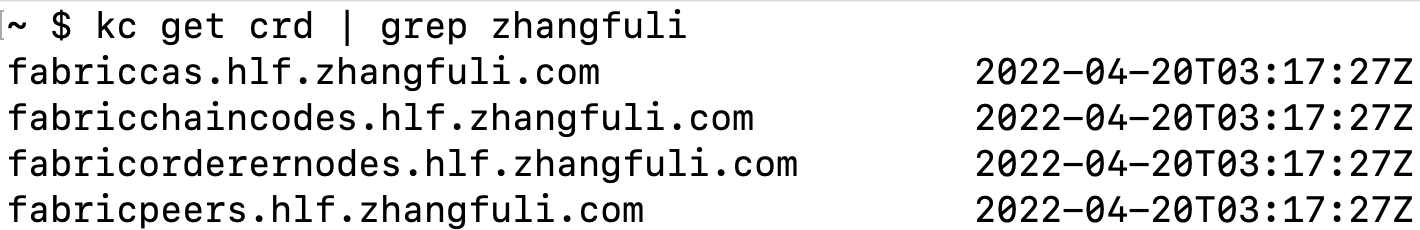
\includegraphics[width=1.0\textwidth]{FIGs/chapter6/crds.png} %中括号中的参数是设置图片充满文档的大小,你也可以使用小数来缩小图片的尺寸。
    \caption{CRD部署结果} %caption是用来给图片加上图题的
    \label{crdresult} %这是添加标签,方便在文章中引用图片。
\end{figure}%figure环境

\textbf{步骤一:} 如表\ref{org1_test}所示, HF网络管理员首先为org1创建了名为“org1-ca”的Ca节点; 其次, 在org1中创建了名为“org1-peer0”的Peer节点,并利用链外存储CouchDB作为账本存储单元。如图\ref{testcase1result}所示为测试结果。

{\footnotesize
\begin{longtable}[h]{m{45pt} m{45pt} m{180pt} m{50pt} m{20pt}}
    \caption[创建Org1测试用例]{Org1测试用例} \label{org1_test}\\
        \toprule  
        \textbf{用例编号}&\textbf{测试编号}&\textbf{用户输入}&\textbf{预期结果}&\textbf{实际}\\
        \hline
        UC-Ca & TC1.1 & 创建名为org1-ca的Ca节点 & 成功启动Ca & 通过 \\
        \hline
        UC-Peer & TC1.2 & 创建名为org1-peer0的Peer节点, 其拥有外部存储CouchDB, 所属于Org1MSP & 成功启动Peer节点 & 通过 \\
        \bottomrule
    \end{longtable} 
}

\begin{figure}[h] %figure环境,h默认参数是可以浮动,不是固定在当前位置。如果要不浮动,你就可以使用大写float宏包的H参数,固定图片在当前位置,禁止浮动。
    \centering %使图片居中显示
    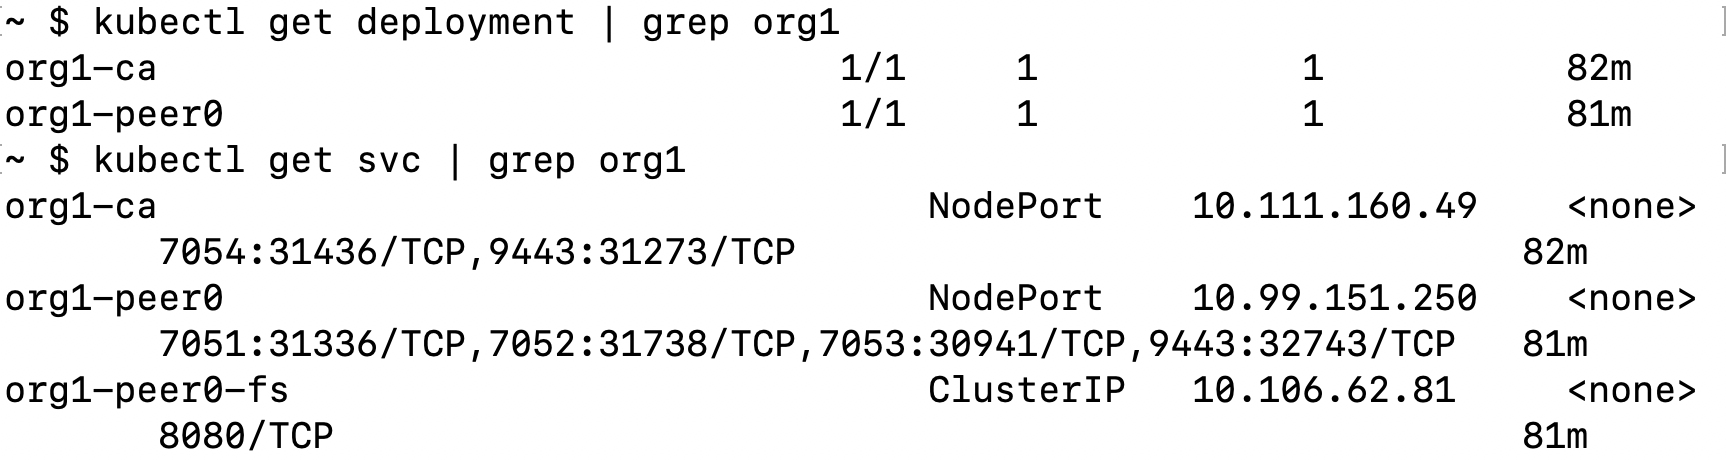
\includegraphics[width=0.9\textwidth]{FIGs/chapter6/peer.png} %中括号中的参数是设置图片充满文档的大小,你也可以使用小数来缩小图片的尺寸。
    \caption{创建Org1测试结果} %caption是用来给图片加上图题的
    \label{testcase1result} %这是添加标签,方便在文章中引用图片。
\end{figure}%figure环境

\textbf{步骤二:} 如表\ref{orderer_test}所示, HF网络管理员需要首先为OrdererMSP创建名为“ord-ca”的Ca节点; 其次, 在OrdererMSP中创建了名为“ord-node1”的Peer节点。如图\ref{testcase2result}所示为测试结果, 原型工具可以为HF网络管理员创建Orderer组织的Ca与Orderer节点, 其中包含但不限于Deployment、Service、Pod、Secret等。

{\footnotesize
\begin{longtable}[h]{m{45pt} m{45pt} m{180pt} m{50pt} m{20pt}}
    \caption[创建Orderer测试用例]{创建Orderer测试用例} \label{orderer_test}\\
        \toprule  
        \textbf{用例编号}&\textbf{测试编号}&\textbf{用户输入}&\textbf{预期结果}&\textbf{实际}\\
        \hline
        UC-Ca & TC2.1 & 创建名为ord-ca的Ca节点 & 成功启动Ca & 通过 \\
        \hline
        UC-Orderer & TC2.2 & 创建名为ord-node1的Orderer节点, 所属于OrdererMSP & 成功启动Orderer节点 & 通过 \\
        \bottomrule
    \end{longtable} 
}

\begin{figure}[h] %figure环境,h默认参数是可以浮动,不是固定在当前位置。如果要不浮动,你就可以使用大写float宏包的H参数,固定图片在当前位置,禁止浮动。
    \centering %使图片居中显示
    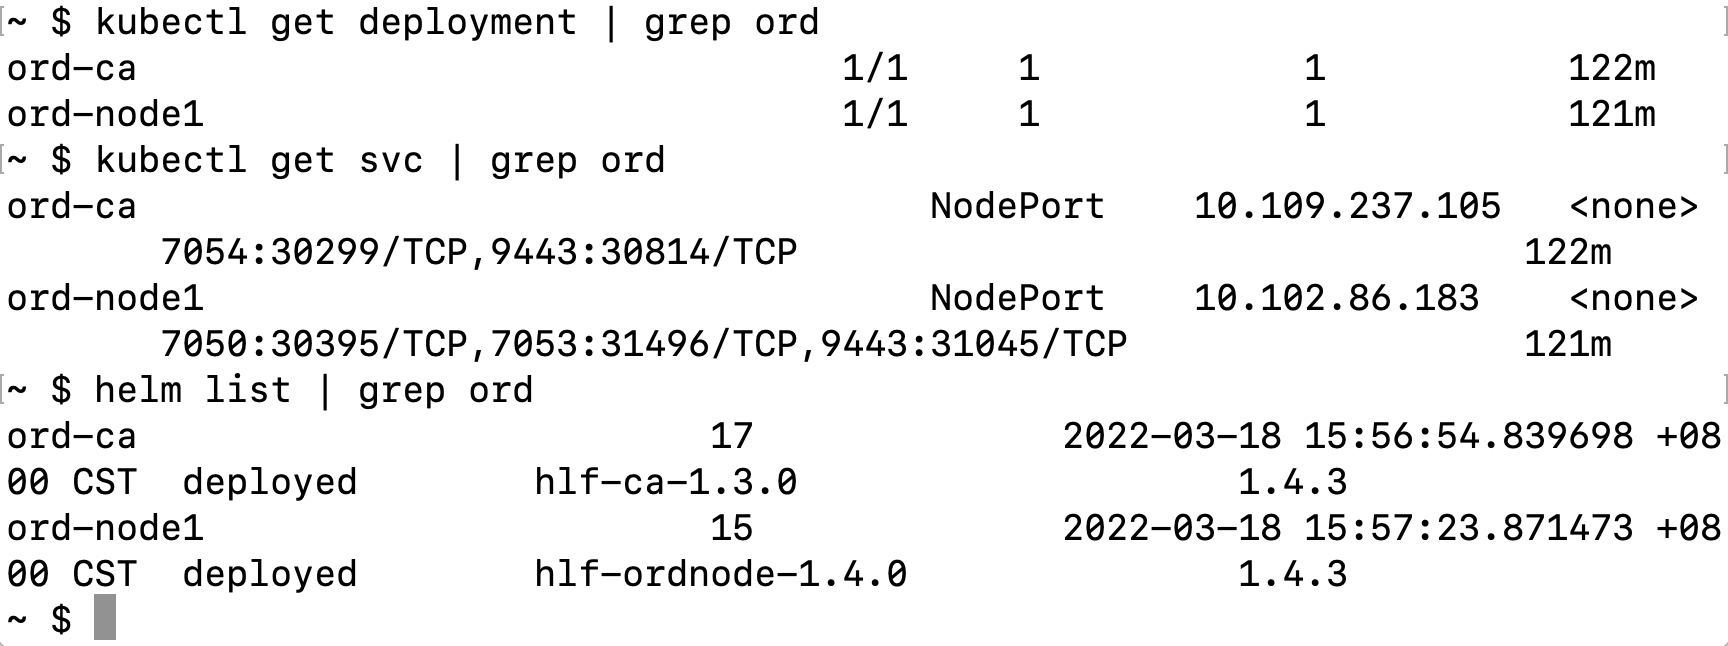
\includegraphics[width=0.9\textwidth]{FIGs/chapter6/orderer.png} %中括号中的参数是设置图片充满文档的大小,你也可以使用小数来缩小图片的尺寸。
    \caption{创建Orderer测试结果} %caption是用来给图片加上图题的
    \label{testcase2result} %这是添加标签,方便在文章中引用图片。
\end{figure}%figure环境

\textbf{步骤三:} 如表\ref{reg_enroll_test}所示, HF网络管理员需要为OrdererMSP以及Org1注册并登记若干用户, 并将用户的证书密钥信息导到Yaml文件中。表中仅展示在Orderer中注册用户, Org1中步骤相似, 注册名为peeruser的用户。测试结果表明, 可以成功将用户及OrdererMSP信息导出。

{\footnotesize
\begin{longtable}[h]{m{45pt} m{45pt} m{180pt} m{50pt} m{20pt}}
    \caption[注册、登记用户测试用例]{注册、登记用户测试用例} \label{reg_enroll_test}\\
        \toprule  
        \textbf{用例编号}&\textbf{测试编号}&\textbf{用户输入}&\textbf{预期结果}&\textbf{实际}\\
        \hline
        UC-Ca & TC3.1 & 为OrdererMSP注册名为ordereruser的用户, 其密码为ordererpw & 成功注册 & 通过 \\
        \hline
        UC-Ca & TC3.2 & 输入用户名密码, 为ordereruser用户登记 & 成功登记,输出证书文件 & 通过 \\
        \bottomrule
    \end{longtable} 
}

\textbf{步骤四:} 如表\ref{channel_test}所示, HF开发人员需要在新创建的HF网络上创建通道, 并初始化该通道内的创世区块。当通道被创建完成之后, 需要将在该通道内进行交易的Orderer、Peer加入该通道。最后, HF开发人员可以指定锚节点并查看通道的高度。如图\ref{channel_test_result}所示为测试结果, 展示了新创建的通道的高度。

{\footnotesize
\begin{longtable}[h]{m{45pt} m{45pt} m{180pt} m{50pt} m{20pt}}
    \caption[创建通道测试用例]{创建通道测试用例} \label{channel_test}\\
        \toprule  
        \textbf{用例编号}&\textbf{测试编号}&\textbf{用户输入}&\textbf{预期结果}&\textbf{实际}\\
        \hline
        UC-Chan & TC4.1 & 选择OrdererMSP为排序组织在Org1MSP上创建通道 & 成功创建通道 & 通过 \\
        \hline
        UC-Chan & TC4.2 & 在通道内创建创世节点 & 成功创建创世节点 & 通过 \\
        \hline
        UC-Orderer & TC4.2 & 将ord-node1加入通道 & 加入成功 & 通过 \\
        \hline
        UC-Peer & TC4.3 & 将org1-peer0加入通道 & 加入成功 & 通过 \\
        \hline
        UC-Chan & TC4.4 & 指定锚节点 & 指定成功 & 通过 \\
        \hline
        UC-Chan & TC4.5 & 查看通道高度 & 查看成功 & 通过 \\
        \bottomrule
    \end{longtable} 
}

\begin{figure}[h] %figure环境,h默认参数是可以浮动,不是固定在当前位置。如果要不浮动,你就可以使用大写float宏包的H参数,固定图片在当前位置,禁止浮动。
    \centering %使图片居中显示
    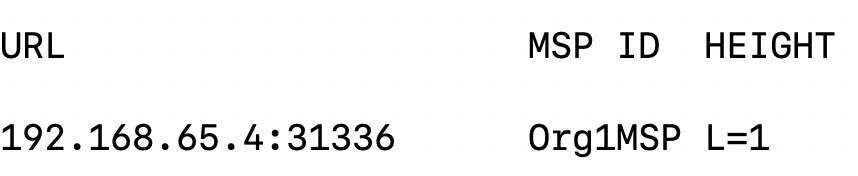
\includegraphics[width=0.6\textwidth]{FIGs/chapter6/channel.png} %中括号中的参数是设置图片充满文档的大小,你也可以使用小数来缩小图片的尺寸。
    \caption{查看通道高度测试结果} %caption是用来给图片加上图题的
    \label{channel_test_result} %这是添加标签,方便在文章中引用图片。
\end{figure}%figure环境

\textbf{步骤五:} 如表\ref{chaincode_test}所示, 为测试通道内所有的参与节点按照链码的合同规则执行, HF开发人员需要在新创建的通道内安装官方提供的asset\footnotemark[1]\footnotetext[1]{\href{https://github.com/hyperledger/fabric-samples/blob/main/asset-transfer-basic/chaincode-go/chaincode/smartcontract.go}{asset链码}}链码, 安装完链码之后, 需要对其进行审批、提交。最后, HF开发人员可以调用链码接口对其进行初始化、查询等一系列操作。如图\ref{chaincode_test_result}所示仅为调用测试结果, 第\ref{section: smart_contract_microservice_test}节已经证明了智能合约微服务化的可行性。

{\footnotesize
\begin{longtable}[h]{m{45pt} m{45pt} m{180pt} m{50pt} m{20pt}}
    \caption[创建通道测试用例]{创建通道测试用例} \label{chaincode_test}\\
        \toprule  
        \textbf{用例编号}&\textbf{测试编号}&\textbf{用户输入}&\textbf{预期结果}&\textbf{实际}\\
        \hline
        UC-CC & TC5.1 & 安装链码并指定语言、label & 安装成功 & 通过 \\
        \hline
        UC-CC & TC5.2 & 查询已经安装的链码 & 查询成功 & 通过 \\
        \hline
        UC-CC & TC5.3 & 审批链码, 并提供链码ID以及策略 & 审批成功 & 通过 \\
        \hline
        UC-CC & TC5.4 & 提交链码, 并提供链码ID以及策略 & 指定成功 & 通过 \\
        \hline
        UC-CC & TC5.5 & 调用链码, 并提供链码调用函数 & 调用成功 & 通过 \\
        \bottomrule
    \end{longtable} 
}

\begin{figure}[h] %figure环境,h默认参数是可以浮动,不是固定在当前位置。如果要不浮动,你就可以使用大写float宏包的H参数,固定图片在当前位置,禁止浮动。
    \centering %使图片居中显示
    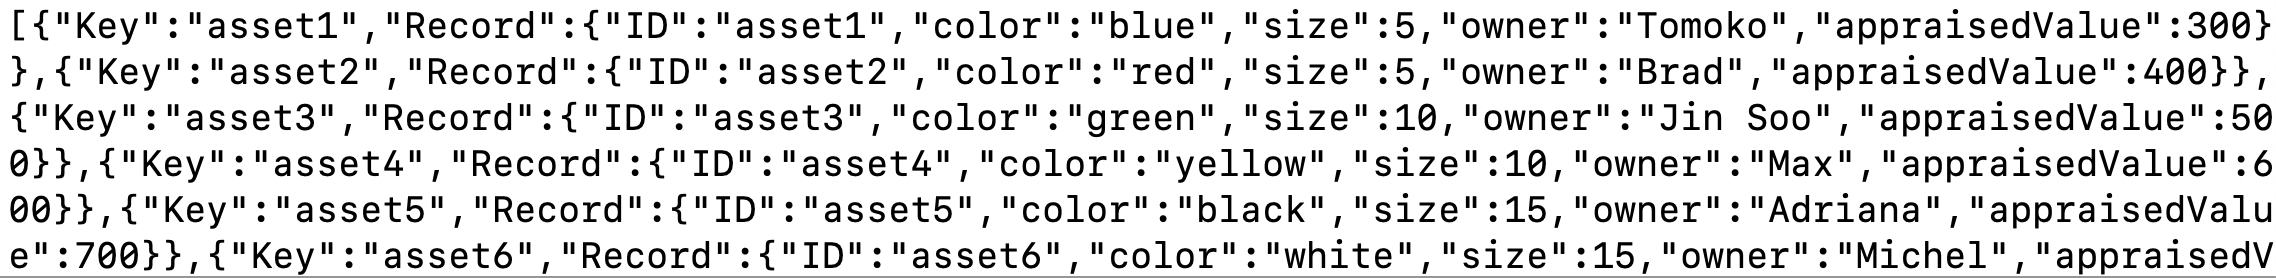
\includegraphics[width=1.0\textwidth]{FIGs/chapter6/chaincode.png} %中括号中的参数是设置图片充满文档的大小,你也可以使用小数来缩小图片的尺寸。
    \caption{查询链码} %caption是用来给图片加上图题的
    \label{chaincode_test_result} %这是添加标签,方便在文章中引用图片。
\end{figure}%figure环境


经过上述步骤1-5, 最终的网络节点状态如图\ref{fabric_result}所示, 本文搭建了一个单Orderer以及单Org、单Peer的经典HF网络, 并分别为Orderer、以及Peer组织搭配Ca证书认证。在搭建了基本的网络之后, 分别为Orderer、Peer注册并登记用户, 最后在组织Org中搭建了一个通道并成功安装调用并链码。由案例分析的结果可知, 本文的区块链云化框架及原型工具能够成功搭建HF网络节点并能够正确地部署、运行链码。

\begin{figure}[h] %figure环境,h默认参数是可以浮动,不是固定在当前位置。如果要不浮动,你就可以使用大写float宏包的H参数,固定图片在当前位置,禁止浮动。
    \centering %使图片居中显示
    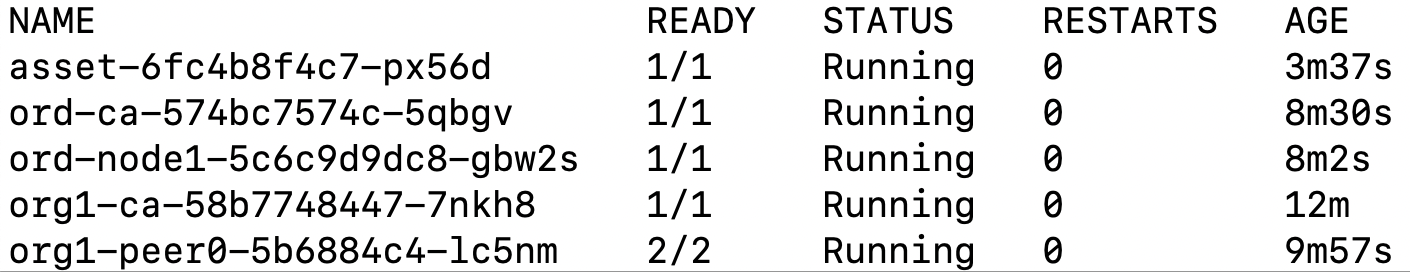
\includegraphics[width=1.0\textwidth]{FIGs/chapter6/fabric_result.png} %中括号中的参数是设置图片充满文档的大小,你也可以使用小数来缩小图片的尺寸。
    \caption{网络节点状态} %caption是用来给图片加上图题的
    \label{fabric_result} %这是添加标签,方便在文章中引用图片。
\end{figure}%figure环境


\subsection{架构评估}

在软件工程中, 常见的评估软件体系结构的方法有Software Architecture Analysis Method(SAAM)、Architecture Trade-off Analysis Method(ATAM), 以上都是基于场景的质量属性评估方法\cite{ionita2002scenario}。SAAM相较于ATAM而言其结构以及评估过程相对简单, 需要准备的工作较少并且SAAM适用于对软件最终版本的评估\cite{huhonglei2004}。本文首先对第\ref{section: framework_characteristics}节所涉及到的设计原则的描述映射到对应的质量属性, 然后采取SAAM方法对其进行评估。

在SAAM评估方法开始之前, 本文邀请了4位熟悉HF基本概念及网络搭建流程的软件开发工程师分别两两扮演HF网络管理员、HF开发人员, 1位熟悉Kubernetes操作的集群运维工程师扮演集群管理员, 以上5位分别为本次SAAM评估方法的风险承担者。本节实施SAAM评估方法涉及以下步骤:

\textbf{1. 场景开发: }所有的风险承担者通过头脑风暴的方式, 提出反应自己需求的场景, 产出结果见步骤3。

\textbf{2. 软件架构描述: }本文详细的为各位风险承担者介绍面向Hyperledger Fabric的区块链云化框架及其原型工具, 包括框架设计理念与原理、原型工具功能和工具实现细节。

\textbf{3. 场景分类: }在这个过程中, 如表\ref{saam_step3}所示, 本文对步骤1所产出的场景进行分类并设定优先级。同时, 在分析时根据场景是否需要修改特定的体系结构把场景分为直接场景与间接场景。

{\footnotesize
\begin{longtable}[h]{m{20pt} m{60pt} m{90pt} m{40pt} m{40pt} m{40pt} m{30pt}}
    \caption[场景分类结果]{场景分类结果} \label{saam_step3}\\
        \toprule  
        \textbf{编号}&\textbf{风险承担者}&\textbf{场景描述}&\textbf{设计原则}&\textbf{质量属性}&\textbf{场景分类}&\textbf{优先级}\\
        \hline
        T1&  HF网络管理员 & 命令式启停HF网络中的任意节点 & 简单易用  & 功能需求 & 直接需求 &  高 \\
        \hline
        T2&  HF网络管理员 & 命令创建HF网络用户 & 简单易用 & 功能需求 & 直接需求 &  高 \\
        \hline
        T3&  HF开发人员 & 命令式创建通道 & 简单易用 & 功能需求 & 直接需求 &  高 \\
        \hline
        T4&  HF开发人员 & 持续交付部署链码 & 简单易用 & 功能需求 & 直接需求 &  高 \\
        \hline
        T5&  HF开发人员 & 命令式操作链码 & 简单易用 & 功能需求 & 直接需求 &  高 \\
        \hline
        T6&  HF网络管理员 \newline HF开发人员 & 能在30min内启动完整网络 & 简单易用 & 易用性 & 间接需求 &  高 \\
        \hline
        T7&  HF网络管理员 & 扩容HF节点资源 & 灵活扩展 & 可扩展性 & 间接需求 &  中 \\
        \hline
        T8&  HF网络管理员 & 扩容账本存储单元 & 灵活扩展 & 可扩展性 & 间接需求 &  高 \\
        \hline
        T9&  HF开发人员 & 保存用户密钥 & 安全可靠 & 安全性 & 间接需求 &  高 \\
        \hline
        T10&  HF开发人员 & 操作网络时需要身份认证 & 安全可靠 & 安全性 & 间接需求 &  高 \\
        \hline    
        T11&  k8s管理员 & HF网络与其他集群程序进行隔离 & 安全可靠 & 安全性 & 间接需求 &  高 \\
        \hline
        T12&  k8s管理员 & Operator限定管理HF网络节点 & 安全可靠 & 安全性 & 间接需求 &  高 \\
        \hline
        T13&  HF网络管理员 \newline HF开发人员 & 良好异常反馈机制 & 安全可靠 & 可靠性 & 间接需求 &  高 \\
        \hline
        T14&  HF网络管理员 \newline HF开发人员 & HF网络节点的全面监控能力 & 可视运维 & 可靠性 & 间接需求 &  高 \\
        \hline
        T15&  HF网络管理员 \newline HF开发人员 & Operator在不同云平台之间迁移的便捷性 & 云链结合 & 可移植性 & 间接需求 &  中 \\
        \bottomrule
    \end{longtable} 
}

\textbf{4. 场景评估: }这个过程重点针对间接场景, 并对其进行评估。针对直接场景, 第\ref{section: tool_test}节已经对其进行了较为全面的功能性测试。

简单易用, 本文同时邀请了这5位风险承担者对本文的原型工具进行易用性测试。为了排除网络的影响,
本文提前下载好原型工具搭建HF网络所需要的Docker镜像。在介绍了本工具的基本原理以及命令行的基本使用方法后, 5位风险承担者分别独立自行搭建不同规格的HF网络, 最终5位风险承担者都能够在30分钟内学习并掌握原型工具的使用方法。


\begin{figure}[h] %figure环境,h默认参数是可以浮动,不是固定在当前位置。如果要不浮动,你就可以使用大写float宏包的H参数,固定图片在当前位置,禁止浮动。
    \centering %使图片居中显示
    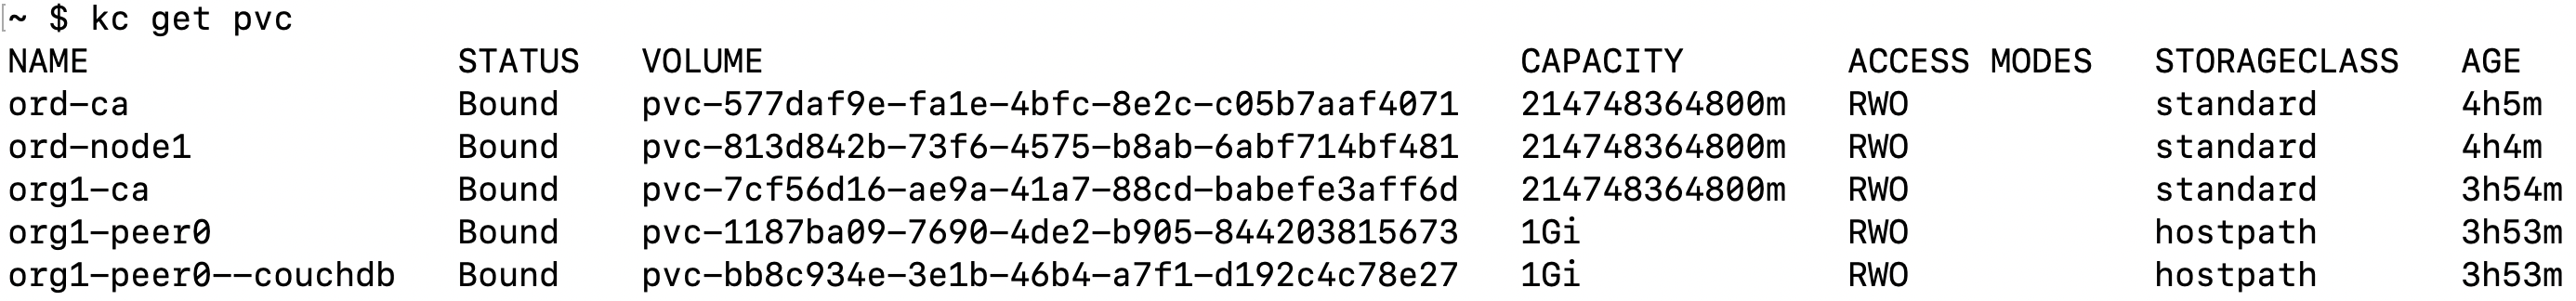
\includegraphics[width=1.0\textwidth]{FIGs/chapter6/db.png} %中括号中的参数是设置图片充满文档的大小,你也可以使用小数来缩小图片的尺寸。
    \caption{网络存储状态} %caption是用来给图片加上图题的
    \label{db} %这是添加标签,方便在文章中引用图片。
\end{figure}%figure环境

灵活扩展, 在HF网络节点资源方面, 由于HF网络节点的CR中配置了HF网络节点运行态时所需的资源(CPU、内存)大小, 所以当对节点CR进行修改时, Controller会监听到CR的变化并更新运行中节点Deployment的资源大小。在数据存储的可扩展性方面,如图\ref{db}所示, 原型工具为每个HF网络中的工作节点设置了专属存储单元。每个存储单元配置专属的PVC管理, HF网络管理员可以不仅可以通过修改节点的CR进行扩容, 可以直接在Kubernetes中对PVC进行动态扩容。值得注意的是, 由于存储单元PVC扩容依赖于StorageClass, 当前只有AWS-EBS、GCE-PD、Azure磁盘、Azure文件、Glusterfs、Cinder、Portworx和Ceph RBD数据卷插件才能支撑数据扩容操作。


安全可靠, 原型工具通过可以以文件形式导出HF网络登记用户产生的密钥信息, 并可以通过Secret进行保存。当这些用户操作HF网络时, 原型工具会要求提供对应的密钥文件作为身份认证的方式。同时, 原型工具将所有的HF资源放在同一命名空间下, 并通过RBAC为该命名空间提供了两种类型的角色。当集群其他用户对已经部署的HF网络节点拥有超越权限的操作时, 原型工具会提示并不进行相关操作。在可靠性方面, 本文在使用原型工具搭建HF网络过程中有意输入错误的命令行参数, 输入不正确的密钥文件等, 原型工具都能在1s内给出参数的异常情况; 同时, 原型工具能够有效利用Prometheus监控体系对工具本身以及HF网络的所有节点、链码以及DB进行监控, 如图\ref{monitoring}展示了利用Prometheus与Grafana对Ca Resource进行监控的画面, 图中展示了Ca CPU的使用情况。在搭建完HF网络之后, 原型工具在两周内仅崩溃1次, 且能通过日志以及Prometheus的告警设置在5分钟内进行恢复。

\begin{figure}[h] %figure环境,h默认参数是可以浮动,不是固定在当前位置。如果要不浮动,你就可以使用大写float宏包的H参数,固定图片在当前位置,禁止浮动。
    \centering %使图片居中显示
    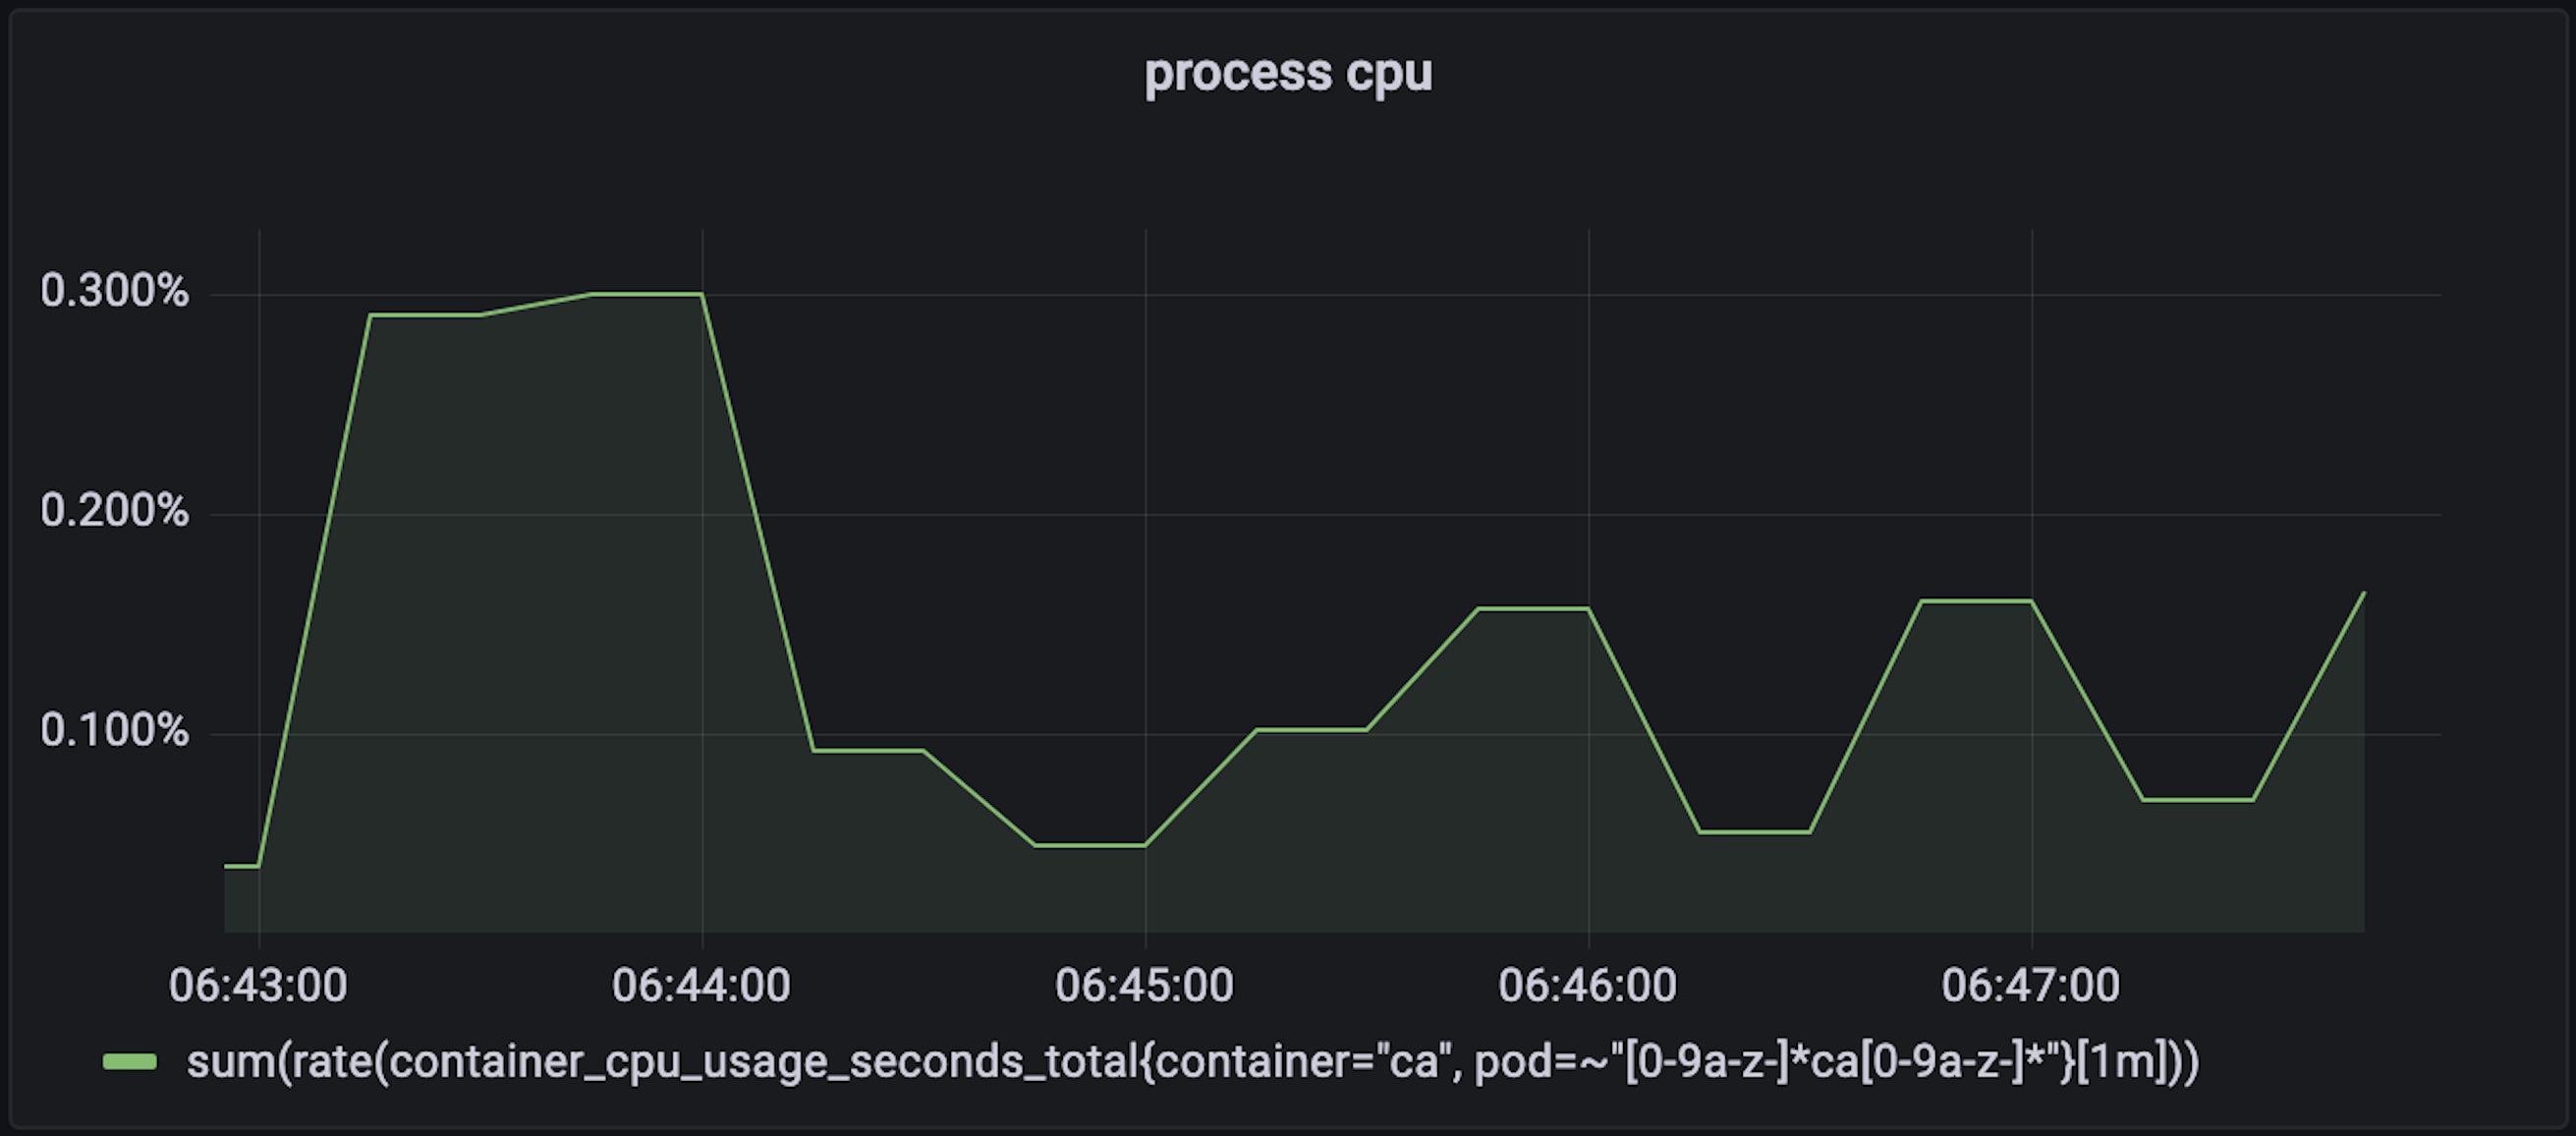
\includegraphics[width=0.9\textwidth]{FIGs/chapter6/ca_cpu.png} %中括号中的参数是设置图片充满文档的大小,你也可以使用小数来缩小图片的尺寸。
    \caption{Ca CPU监控图} %caption是用来给图片加上图题的
    \label{monitoring} %这是添加标签,方便在文章中引用图片。
\end{figure}%figure环境

云链结合, 重点是在可移植性下的场景。本文通过Dockerfile将本工具打包成Docker镜像\footnotemark[1]\footnotetext[1]{\href{https://hub.docker.com/repository/docker/zhangfuli/hfoperator}{HFOperator镜像}}, 使用预先打包并经过检验的镜像, 并为该原型工具配备专用的Helm chart, 其中包含有关原型工具构建的所有必要信息, 这样可以以最少的时间部署。结果表明, 原型工具可以通过Helm在支持Kubernetes 1.18版本以上的云平台上运行, 原型平台具备良好的可移植性。

\textbf{5. 总体评估: }本文的原型工具可以有效利用Kubernetes Operator云化策略来提升HF网络节点的易用性、可扩展性、安全性、以及可靠性。


\section{成熟度衡量}

\begin{figure}[h] %figure环境,h默认参数是可以浮动,不是固定在当前位置。如果要不浮动,你就可以使用大写float宏包的H参数,固定图片在当前位置,禁止浮动。
    \centering %使图片居中显示
    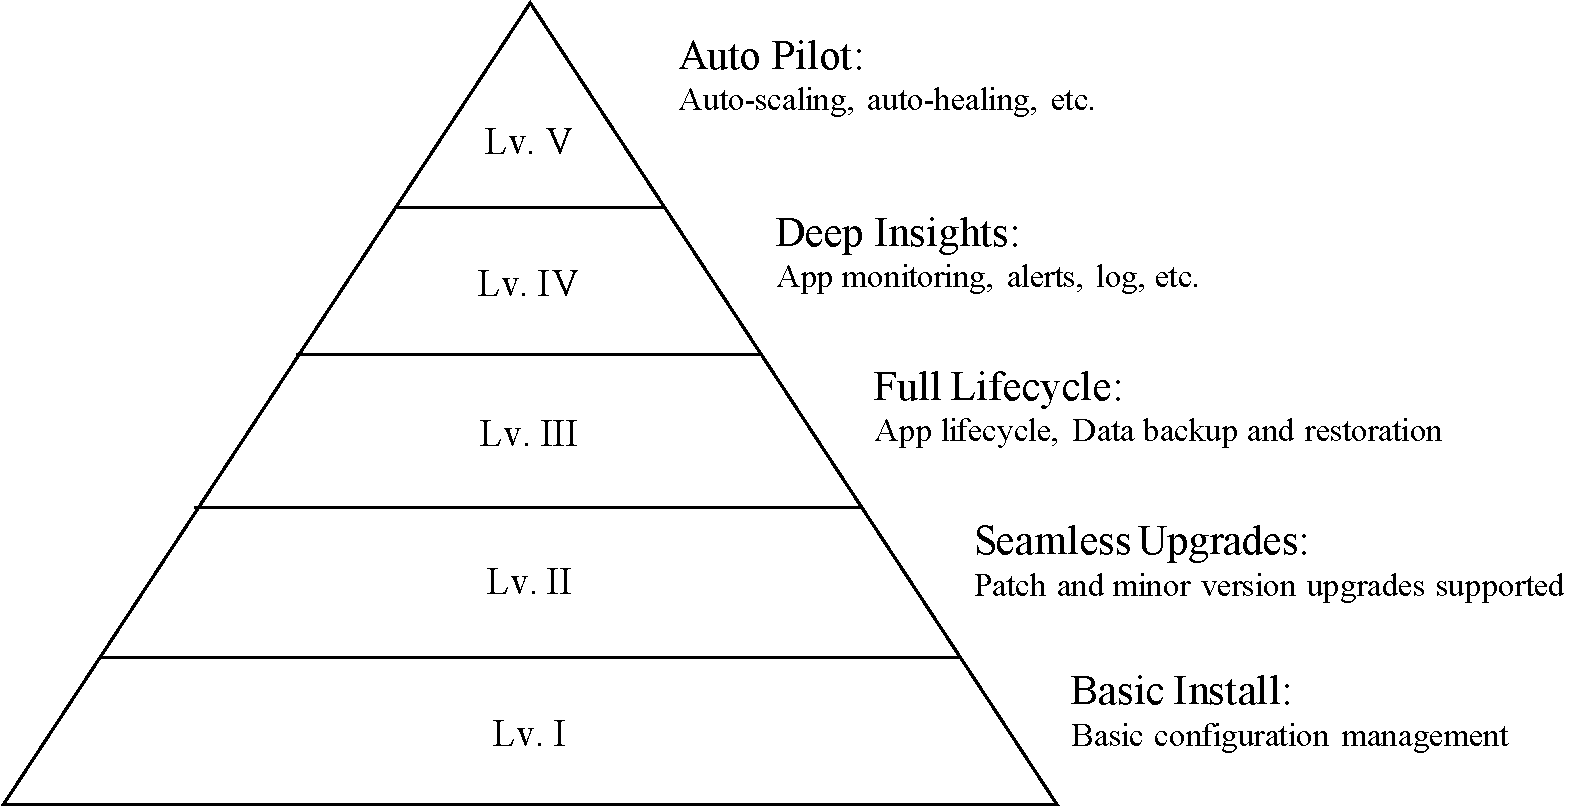
\includegraphics[width=0.95\textwidth]{FIGs/chapter6/maturity.pdf} %中括号中的参数是设置图片充满文档的大小,你也可以使用小数来缩小图片的尺寸。
    \caption{成熟度模型} %caption是用来给图片加上图题的
    \label{maturity} %这是添加标签,方便在文章中引用图片。
\end{figure}%figure环境


如图所示\ref{maturity}, Kubernetes Operator拥有5个成熟度级别的定义\cite{duan2021case}, 其通过定性的方式分析某个Operator应用是否达到了某个级别, 这5个成熟度级别定义如下:

\begin{itemize}[itemindent=2em]
    \item 第一级: Basic Install, 该级是Operator成熟度模型中最基本的级别。在该级中, 用户能够使用CRD对目标程序进行配置和安装;

    \item 第二级: Seamless Upgrades, 在该级别上的Operator能够不丢失数据的升级所管理的工作负载;

    \item 第三级: Full Lifecycle, 是否能达到该级别取决于Operator是否具备生命周期管理和的数据备份、恢复能力。在该级别上的Operator能够备份数据, 并在发生任何数据灾难时从备份数据中恢复数据;

    \item 第四级: Deep Insights, Operator提供监控和报警等功能。在该级别, Operator能够包含所有组件的运行状况指标, 并根据指标配备报警功能;

    \item 第五级: Auto Pilot, 最终级别拥有许多高级功能, 如自动伸缩。Operator可以根据收集到的指标来扩展工作负载。

\end{itemize}

\textbf{Basic Install}

借助于原型工具, 用户能够通过命令行方式一键启停HF网络中任意节点, 而且不需要进行复杂的证书管理。一旦原型工具被部署在Kubernetes网络中, 原型工具就可以对CR以及Helm进行管理, HF网络管理人员可以借助命令行参数的方式进行创建、更新CR以此来创建特定规格的HF网络。 一旦CR进行更新, 原型工具就会将当前状态调整为与指定状态一致。

\textbf{Seamless Upgrades}

在原型工具中, HF网络管理员可以通过修改CR的内容对包括HF网络节点镜像、端口、Host、版本等进行无缝修改。此外, 由于原型工具依赖于链外存储的CouchDB以及外部的Prometheus监控体系, 这两者的升级并不会对原型工具产生严重的负面影响。 

\textbf{Full Lifecycle}

虽然原型工具能够在Mangager中对结合Helm对HF网络进行全生命周期管理, 但目前原型工具目前仍缺少数据备份和恢复的能力。要达到这一能力需要在CR中指定远程备份的数据存储平台, 并在CR中指定数据备份的凭证以及远程备份的链接。同时, 原型工具需要在一定的时间周期内将数据备份到远程的数据存储平台上。

\textbf{Deep Insights}

原型工具利用Prometheus监控体系实现监控与报警的功能, 与此同时, 除了利用Prometheus抓取Pod的基本指标外, CRD中还设定了PodMonitor、ServiceMonitor、CouchDBExporter接口, 可以让Prometheus更全面的抓取HF网络的监控指标。HF网络管理员可以通过Grafna可视化图表查看整体HF网络运行状态, 并且能够根据监控指标创建自定义的告警规则。

\textbf{Auto Pilot}

在Kubernetes中存在两种自动伸缩的插件, 即HPA、VPA。当负载超过一定的阈值时, 就会对其进行伸缩或配置更多的资源。然而在HF网络中, 每个Peer都有记录全部账本的职责, 并且只需要超过51\%的Peer节点保持一致即可, 所以针对于Peer并不需要根据监控进行自我伸缩的能力。在数据存储方面, 随着账本的膨胀, 原型工具可以针对链外存储进行扩容。

综上, 通过定性分析, 本文原型工具利用Operator管理HF网络能够完美的具备第一级、第二级的能力, 在第三级上能够支持全生命周期管理但是对于数据的备份能力依旧是存在欠缺, 借助Prometheus实现了第四级的监控, 对于自动伸缩方面支持资源及数据层面的扩展, 所以本文原型工具基本满足5层成熟度模型的功能。

\section{对比分析} \label{section: tool_comparison}

除上述通过定性分析的手段对原型工具进行评估外, 本文选取了Hyperledger官方推出的BaaS平台Cello进行定量的对比分析。本文重点关注的是对HF网络节点的云化问题, 所以需要在网络部署时间与链码交付时间上对Cello以及原型工具进行对比。

本文在云主机环境下拉取Cello的release-0.9.0-h3c并进行打包构建以及运行。Cello通过图形化的Cello Operator进行主机绑定、组织管理、网络管理以及用户管理。操作Cello Operator的就是HF网络管理员, 管理员首先在主机管理中添加主机, 主机就是Cello将要部署的目标Docker或者Kubernetes环境, 然后再依次创建组织并启动网络, 整个过程全都通过图形化界面的方式完成。

% 如图\ref{cello}所示,
% \begin{figure}[h] %figure环境,h默认参数是可以浮动,不是固定在当前位置。如果要不浮动,你就可以使用大写float宏包的H参数,固定图片在当前位置,禁止浮动。
%     \centering %使图片居中显示
%     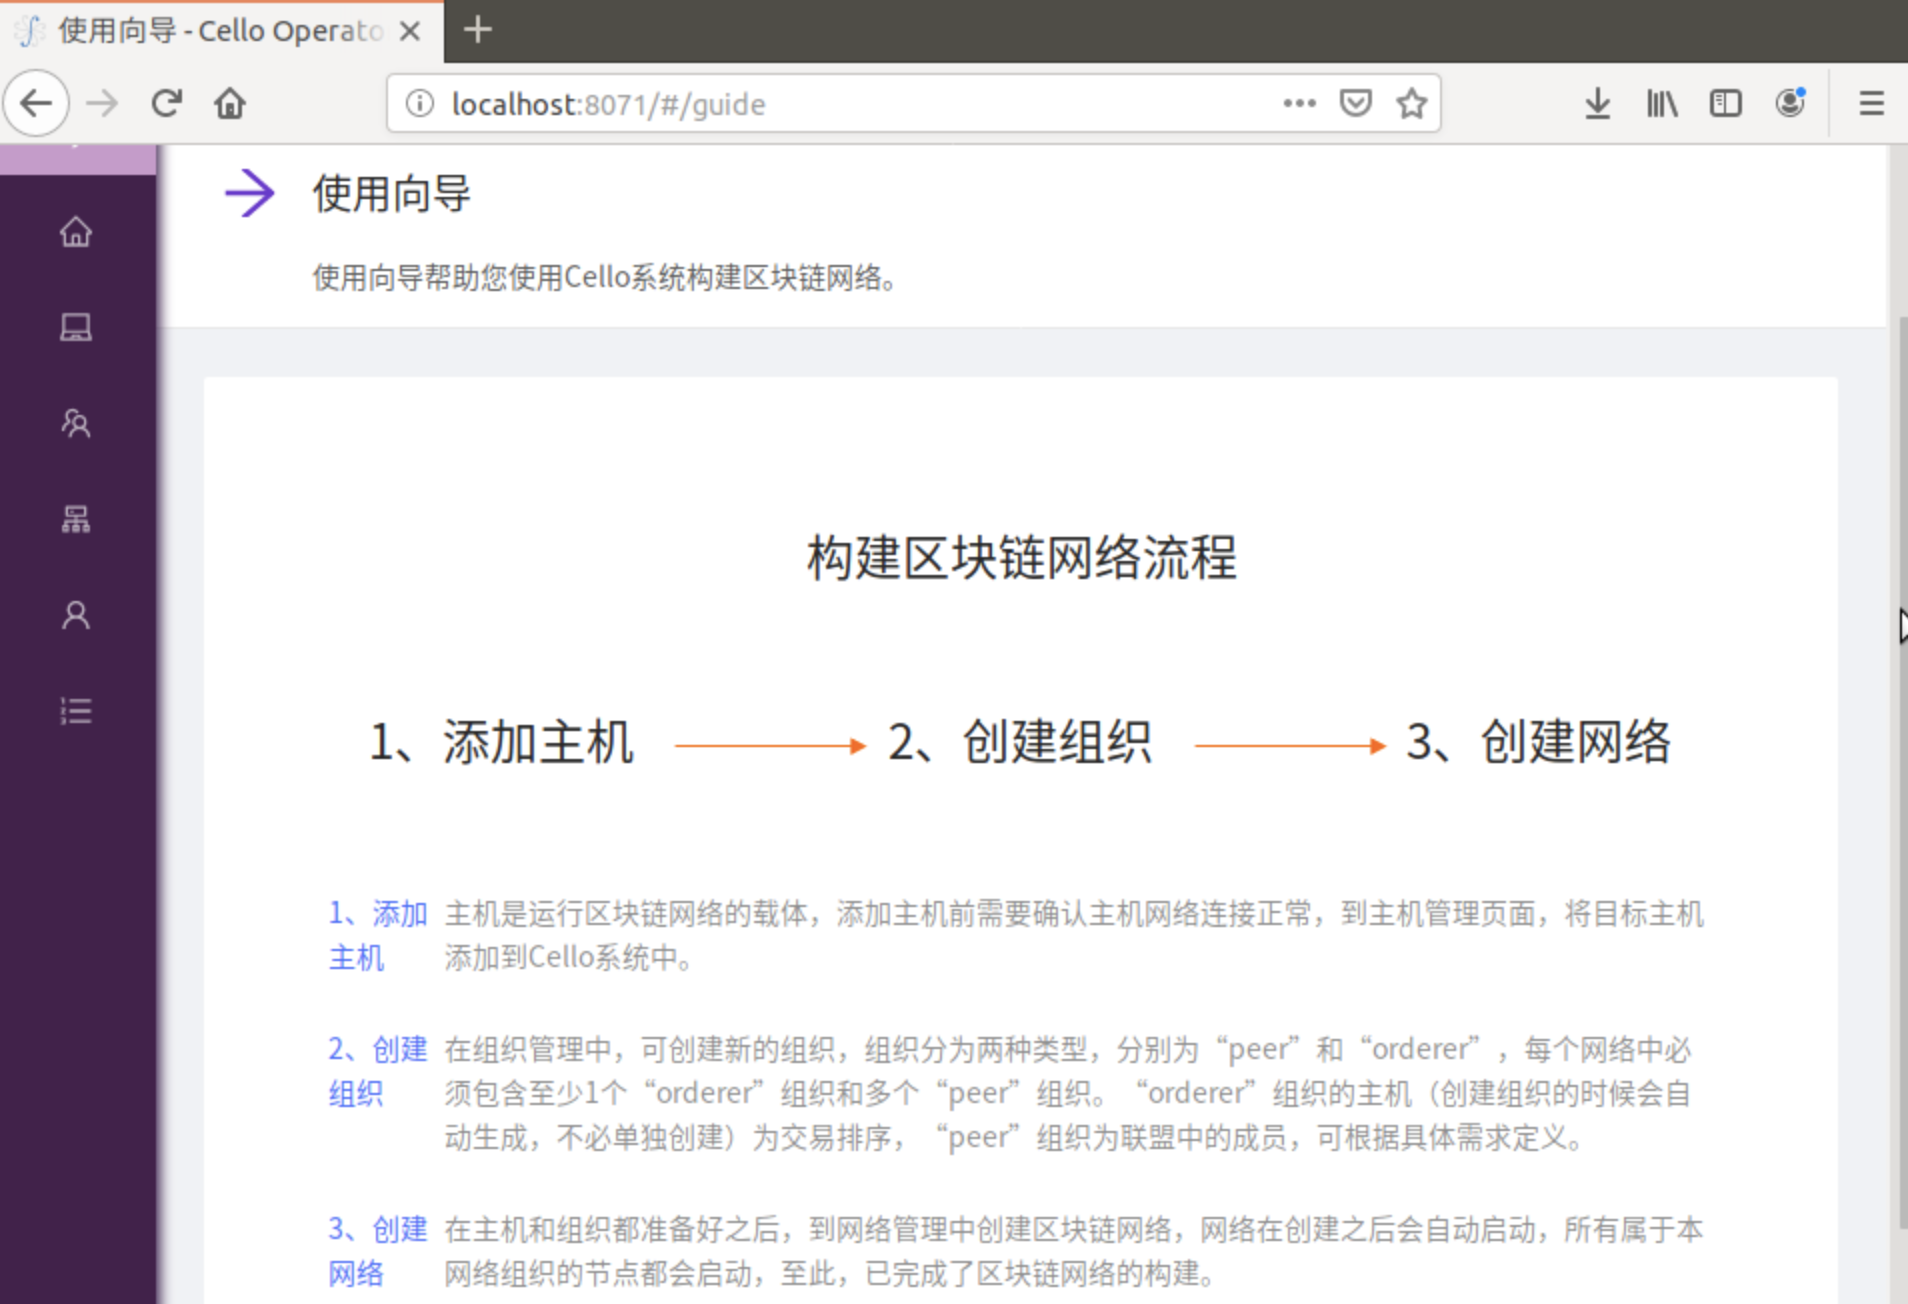
\includegraphics[width=0.95\textwidth]{FIGs/chapter6/cello.png} %中括号中的参数是设置图片充满文档的大小,你也可以使用小数来缩小图片的尺寸。
%     \caption{图形化Cello Operator} %caption是用来给图片加上图题的
%     \label{cello} %这是添加标签,方便在文章中引用图片。
% \end{figure}%figure环境


{\footnotesize
\begin{longtable}[h]{m{100pt} m{100pt} m{100pt}}
    \caption[Hyperledger Fabric版本信息]{Hyperledger Fabric版本信息} \label{test_fabric_net} \\
        \hline  
        \textbf{镜像}&\textbf{Cello版本}&\textbf{原型工具版本}\\
        \hline
        Fabric-Ca & 1.4.2 & 1.4.9 \\
        Fabric-Peer & 1.4.2 & 2.4.1 \\
        Fabric-Orderer & 1.4.2 & 2.4.1 \\
        \hline
    \end{longtable}
}

由于现在在Docker环境中部署HF网络仍旧是主流, 所以本文利用Cello在Docker中部署作为测试基准。由于Cello的局限性, 仅支持在部署HF网络的1.4版本, 而原型工具能更优地支持HF网络2.X以上版本。
如表\ref{test_fabric_net}展示了本次工具对比所部署的HF网络各节点的版本信息, 测试基准为基于单组织单Peer的网络部署时间, 共识算法选择Solo, 数据存储选择LevelDB。


为了避免人为的手工干扰, 获得更加准确的网络部署时间。本文提前在Cello Operator中创建好Orderer以及org1组织并为每个组织配置一个对应的节点。当点击提交网络时开始计时, 刚开始创建时, 网络节点的状态是“故障”, 当网络节点的状态从“故障”变成“正常”时停止计时, 随后删除该网络。重复10次上述操作, 且为避免后端镜像遗留干扰, 每次操作间隔3min~5min。在原型工具中, 为避免手工输入命令而带来的人为误差, 本文预先编写好创建网络的脚本, 脚本中创建10次网络, 创建完成后删除该网络并在删除后休眠30s, 如此循环10次共得到10次网络启动时间如表\ref{net_deployment_time}所示。

{\footnotesize
\begin{longtable}[h]{m{35pt}|m{40pt}|m{15pt} m{15pt} m{15pt} m{15pt} m{15pt} m{15pt} m{15pt} m{15pt} m{15pt} m{15pt}|m{20pt}}
    \caption[网络部署时间(单位: 秒(s))]{网络部署时间(单位: 秒(s))} \label{net_deployment_time}\\
        \hline
        \multirow{2}*{工具类型}
        & \multirow{2}*{\parbox[c]{40pt}{节点类型}}
        & \multicolumn{10}{c|}{序号}
        
        & \multirow{2}*{\parbox[c]{20pt}{平均}}\\
        \cline{3-12}
        & & 1 & 2 & 3 & 4 & 5 & 6 & 7 & 8 & 9 & 10 & \\
        \hline
        Cello & 整体网络 & 73 & 119 & 115 & 90 & 73 & 89 & 137 & 85 & 103 & 127 & 101.1\\
        \hline  
        \multirow{5}*{\parbox[c]{40pt}{原型工具}}
        & ca(peer) & 13 & 12 & 13 & 13 & 13 & 13 & 13 & 12 & 12 & 12 & 12.6 \\
        & peer & 20 & 21 & 29 & 16 & 23 & 27 & 20 & 20 & 16 & 22 &  21.4 \\
        & ca(ord) & 13 & 13 & 13 & 13 & 13 & 13 & 14 & 13 & 15 & 15 & 13.5 \\
        & orderer & 27 & 36 & 34 & 24 & 33 & 24 & 27 & 25 & 32 & 25 & 28.7 \\
        \cline{2-13}
        & 整体网络 & 73 & 82 & 89 & 66 & 82 & 77 & 74 & 70 & 75 & 74 & 76.2\\
        \hline
    \end{longtable} 
}

\begin{figure}[h] %figure环境,h默认参数是可以浮动,不是固定在当前位置。如果要不浮动,你就可以使用大写float宏包的H参数,固定图片在当前位置,禁止浮动。
    \centering %使图片居中显示
    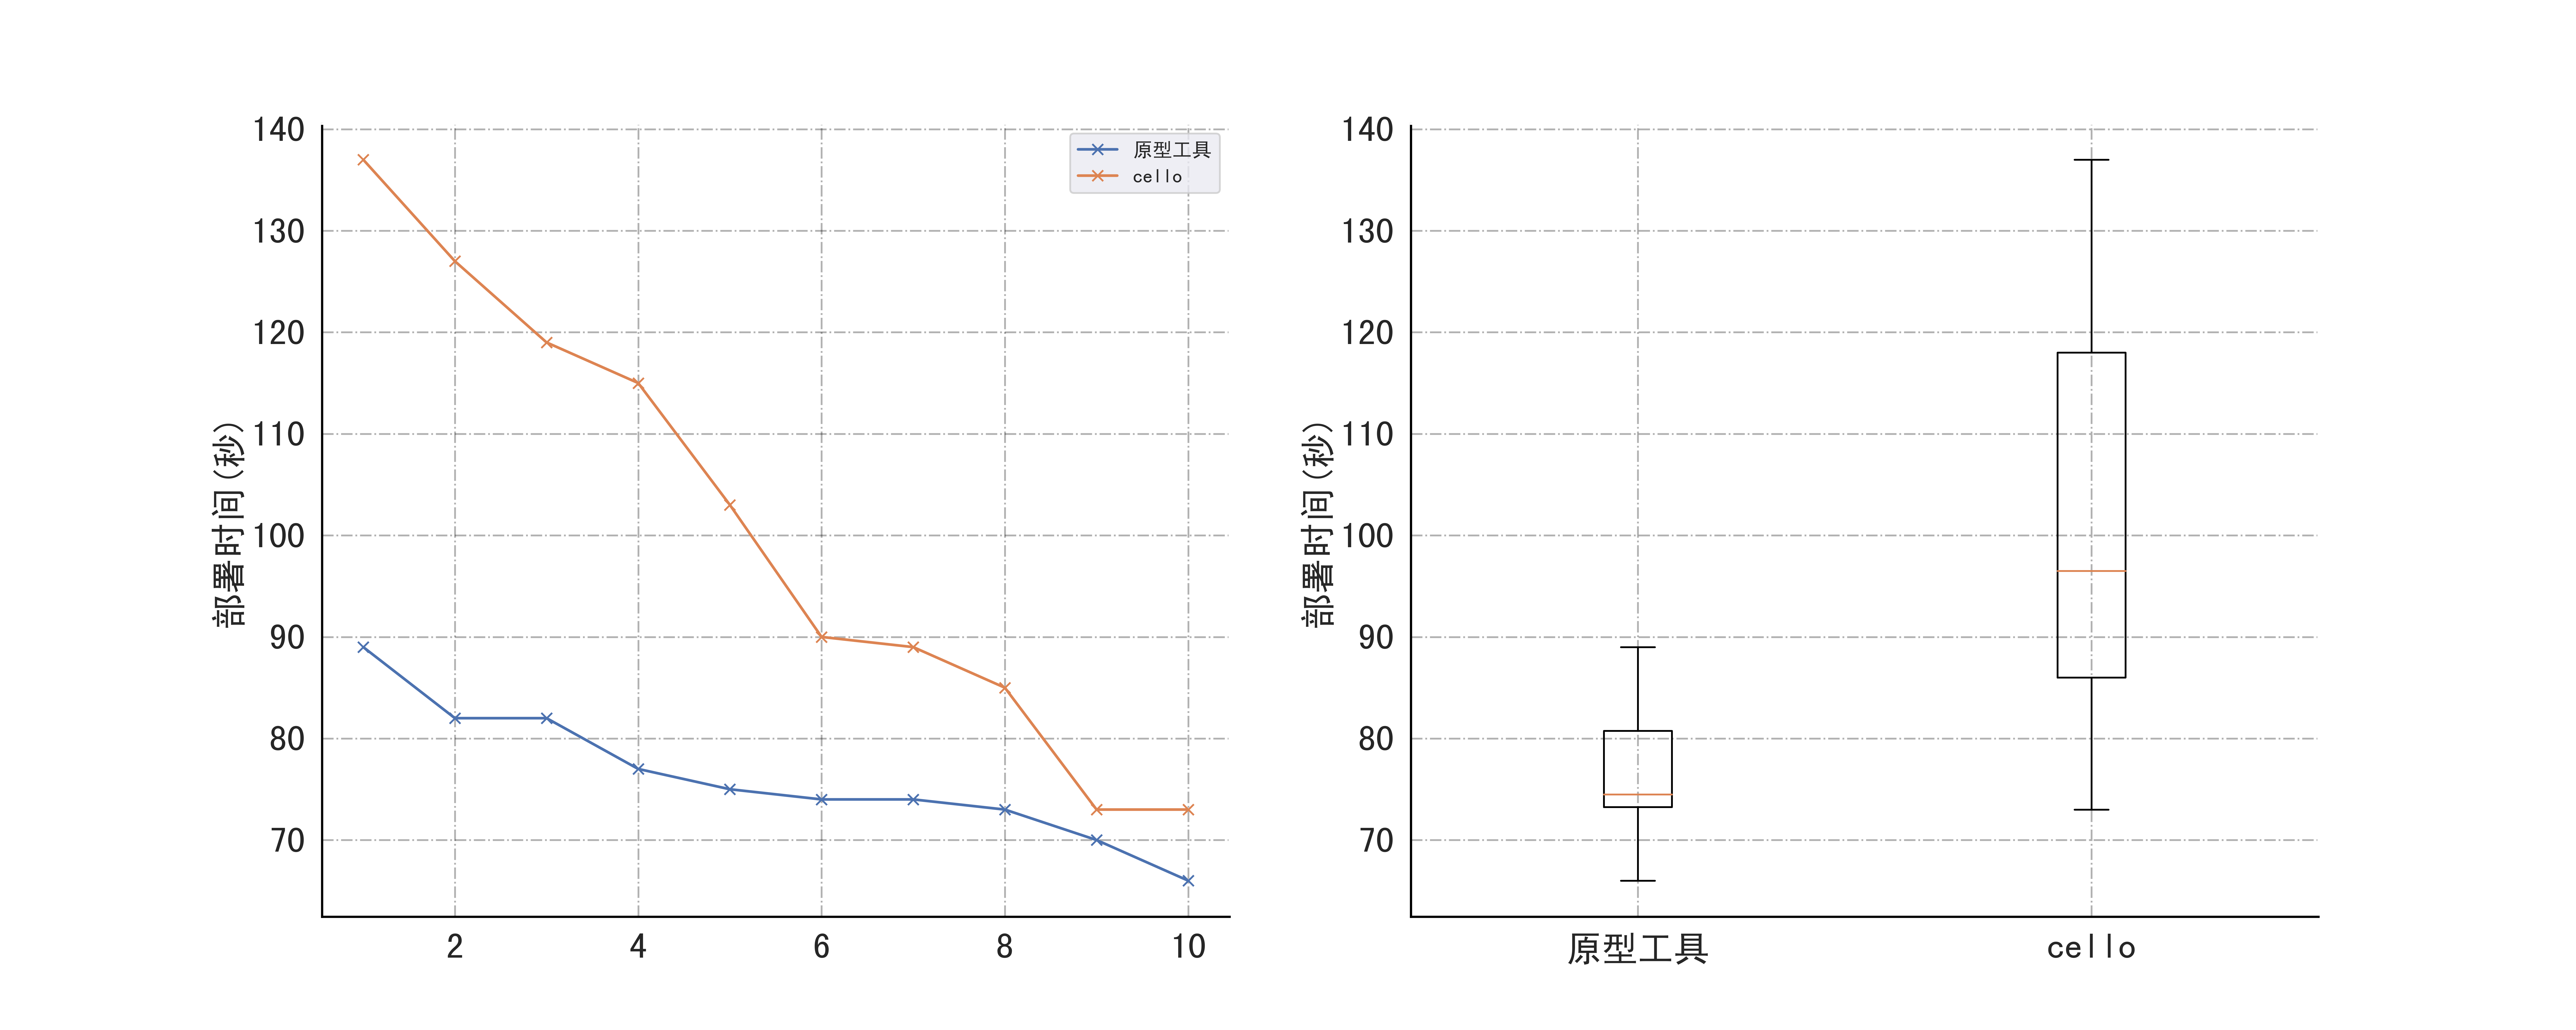
\includegraphics[width=1.0\textwidth]{FIGs/chapter6/plt_deployment.png} %中括号中的参数是设置图片充满文档的大小,你也可以使用小数来缩小图片的尺寸。
    \caption{网络部署时间对比图} %caption是用来给图片加上图题的
    \label{plt_deployment} %这是添加标签,方便在文章中引用图片。
\end{figure}%figure环境

如图\ref{plt_deployment}展示了原型工具和Cello分别部署HF网络的对比图。值得注意的是, 由于Cello采用图形化界面无法配置单个Ca的启停, 所以采用Cello部署的单Orderer单组织的HF网络仅在单个组织内部启动了一个Ca节点, 共计3个网络节点。 而采用原型工具部署的单Orderer单组织的HF网络分别为Orderer以及单组织部署了一个Ca节点, 共计4个网络节点。图\ref{plt_deployment}左侧展示了10次部署排序后的时间曲线图, 图中可以较为直观的看到原型工具比Cello部署的时间要少, 原型工具部署整体网络的平均时间为76.2秒, 而Cello部署整体网络的平均时间为101.1秒; 经计算, 原型工具的总体标准偏差约为6.29, Cello的总体标准偏差约为21.41。图\ref{plt_deployment}右侧分别展示了两者的箱线图, 结合标准偏差可知原型工具部署时间相对而言更为稳定, 尤其在部署Ca节点时, 稳定在13秒左右。

通过分析源码\footnotemark[1]\footnotetext[1]{\href{https://github.com/hyperledger/cello/blob/release-0.9.0-h3c/src/modules/blockchain_network.py}{cello create network}}可知, 当在Cello Operator前端中提交网络之后, Cello对应的Docker Agent会循环解析传入的HF网络节点信息及数量的数据结构, 解析完成后串行构建HF网络中的各类节点。构建过程中, 生成Docker Compose文件并启动对应的网络节点。同样, 当Cello选择在Kubernetes部署时根据Template模板在代码中硬编码生成Yaml文件。由此可得, Cello网络部署时间会随着HF网络中节点数量的增加而线性递增。本文的原型工具, 因需要手动以命令方式部署对应的网络节点, 其部署时间也会随着节点数量增加而递增。因此, 只对单Orderer单Peer进行对比测试即可预估出不同网络规模下的网络部署时间。

在链码部署方面, Cello与原型工具都需要经过创建通道、将账本节点加入至通道内、安装链码等过程。在Cello中上述过程均在图行化界面中配置完成, 原型工具通过命令行方式构建。这两者在安装链码这个环节均在1s内完成, 这对于HF开发人员而言都是能够接受的, 所以这两者仅在安装链码这个环节不需要进行对比。智能合约微服务化的优势在于将智能合约进行解耦, 将智能合约单独作为可交付物。同时开发人员可以利用传统成熟的工具链扩充智能合约开发运维领域的工具空白, 利用已有成熟工具对智能合约进行持续测试、持续交付与持续监控。

{\footnotesize
\begin{longtable}[h]{m{35pt}|m{15pt} m{15pt} m{15pt} m{15pt} m{15pt} m{15pt} m{15pt} m{15pt} m{15pt} m{15pt}|m{20pt}}
    \caption[链码交付时间(单位: 秒(s))]{链码交付时间(单位: 秒(s))} \label{cc_deployment_time}\\
        \hline
        \multirow{2}*{工具类型}
        & \multicolumn{10}{c|}{序号}
        & \multirow{2}*{\parbox[c]{20pt}{平均}}\\
        \cline{2-11}
        & 1 & 2 & 3 & 4 & 5 & 6 & 7 & 8 & 9 & 10 & \\
        \hline
        Cello  & 141 & 128 & 185 & 153 & 166 & 105 & 137 & 160 & 186 & 117 & 147.7\\
        \hline  
        \multirow{1}*{\parbox[c]{40pt}{原型工具}}
        & 119 & 89 & 100 & 76 & 104 & 140 & 136 & 125 & 83 & 164 &  113.6 \\
        \hline
    \end{longtable} 
}

本文对比链码部署过程中所有消耗的时间, 即HF开发人员编写完链码后到将链码成功部署于HF网络节点上所用的时间。如表\ref{cc_deployment_time}展示了原型工具和Cello分别部署asset链码所用的时间对比表。Cello部署链码依次为: 创建通道、加入节点、代码仓库下载链码、压缩链码、计算压缩包MD5、上传链码、安装链码; 原型工具在持续交付流水线中的流程为: 创建通道、加入节点、代码仓库下载链码、打包链码镜像、安装链码。值得注意的是, 本次由于人工操作以及网络波动等情况, 数据可能会存在偏差。最终, Cello的部署链码的平均时间为147.7秒, 原型工具部署链码的平均时间为113.6秒。

综上, 本节对Cello与原型工具进行了定量的对比分析。在网络节点部署方面, 本文原型工具相较于Cello在具有更优的节点部署时间, 并且每次节点部署时间更加稳定。虽然在链码的部署时间方面原型工具表现的较为良好, 但智能合约微服务化的开发运维流程相较于Cello固定式的部署流程能够在流水线中纳入更多的环节如智能合约代码质量、安全等, 以促进智能合约更全面的发展。

\section{本章小结}

本章介绍了对原型工具的测试与评估。首先介绍了本文涉及到的两个测试环境, 并进行了三个维度的评估工作: (1)基本能力自证, 利用典型案例研究的方式进行功能可行性测试, 利用SAAM架构评估方式进行质量属性验证; (2)成熟度衡量, 利用五层成熟度模型的定性评估;(3)对比分析, 与Cello对比的定量分析。


\chapter{总结与展望}

\section{总结}

区块链网络具有去中心化、不可伪造、不可篡改的特性, 其被称为下一代的新型生产关系。随着区块链概念的普及, 其为供应链、金融等传统领域带来了巨大变革。当前, 去中心化应用逐步从概念验证阶段转变为工程化实践阶段。在去中心化应用落地的过程中, 在区块链网络的构建上消耗了大量的时间成本。BaaS基于包括云容器集群在内的云原生技术体系可以帮助区块链开发人员构建、管理、托管区块链网络, 这降低了去中心化应用的落地门槛。

然而, 当前BaaS平台依旧存在着诸多挑战。首先是商业化应用工具不完善, 当前BaaS平台由云提供商巨头把控, 行业马太效应明显。不同云厂商拥有其独立的BaaS平台, 缺乏顶层规划导致多云网络及区块链数据孤岛。其次, 虽然各个云厂商拥有独立的BaaS平台及其相关生态, 但本质上还是将云原生平台作为部署环境, 仅提供一种类似于脚本化部署区块链网路的功能, 远未挖掘云原生底层弹性伸缩、安全性等特性。

因此, 本文针对上述存在的挑战, 本文提出了一种面向Hyperledger Fabric的区块链云化框架。由于Kubernetes Operator可以将领域知识有效的集成到云原生基础设施, 充分发挥云原生的特性。因此本文首先对Kubernetes Operator进行快速评审, 快速评审的范围涵盖了计算机与软件工程领域的4个权威全文数据库并将Scoups和谷歌学术作为补充。将得到的51篇论文经过筛选得到15篇, 对这15篇论文进行数据抽取获得了基于Kubernetes Operator云化的策略集。针对策略集中的策略在区块链背景中进行适配获得了具体区块链云化的具体实施方案。

其次, 根据区块链云化的具体实施方案设计实现了面向Hyperledger Fabric的区块链云化框架及其原型平台。云化框架及其原型平台利用Operator将分别管理HF网络中的Ca、Orderer、Oeer节点。CRD作为框架的输入, 根据官方功能以及配置对节点的属性进行可插拔配置, 如Ca节点的CRLSizeLimit、Orderer节点的Genesis、Peer节点的LevelDB/CouchDB; Manager作为中枢处理单元, 通过对应三个Controller对上述三个节点进行协调循环, 时刻保持节点状态在期望状态。同时, 本文结合实施方案中的策略来提升框架及HF网络的的可迁移性、数据可扩展性、安全性以及可视运维的能力并支持通过命令行方式启停HF网络节点; HF网络作为输出, 包含维持HF网络节点稳定运行的Deployement、Service等Kubernetes配置。

最后, 本文对原型工具进行了全面的测试与评估。以典型案例的方式搭建了单Orderer单组织的HF网络进行功能性测试, 并能够利用云原生的特性满足工具的易用性、可扩展性、安全性等非功能性需求; 在框架及原型工具的评估方面, 本文不仅采用定性分析的方式结合五层成熟度模型对原型工具进行评估而且采用定量分析的方式对比HF官方BaaS平台Cello在网络部署时间上进行了全面对比。结果表明, 原型工具基本满足五层成熟度模型的功能且在部署时间和时间稳定性上优于Cello。


本文提出的面向Hyperledger Fabric的区块链云化框架及其原型工具依托于Kubernetes基础设施, 可以方便的迁移到支持Kubernetes的任何云, 包括公有云、专有云以及混合云, 打破云厂商的垄断格局; 利用输入本应由领域专家执行的参数与操作, 减轻HF网络管理员的负担。利用Kubernetes Operator更原生的管理HF网络, 复用Kubernertes API的公共功能, 如PVC存储、资源隔离、内置认证等方式更好的发挥云原生的潜能, 提升HF网络的易用性、可迁移性、数据可扩展性、安全性以及可视运维的能力。

\section{局限}

本文搭建了原型平台并与Cello进行对比验证, 虽然原型平台在网络部署时间上优于Cello, 但本文提出的面向Hyperledger Fabric的区块链云化框架及其原型工具依旧还有很多局限性:

\begin{itemize}[itemindent=2em]
    \item 为轻量级、快速的将已有知识转移到实践中, 在区块链云化框架调研过程中采用了快速评审的方式, 其相对于系统文献综述(Systematic literature reviews, 简称SLRs)而言缺乏更加深层次的知识掌握。同时Kubernetes Operator以及云原生技术体系在工业界应用广泛而本文的快速评审面对的对象重点是学术工作, 未对灰色文献进行调研。

    \item 本文的Manager中枢控制系统利用Controller对Helm进行进行生命周期监控, 并通过CRD的配置对Helm value进行参数传递。这种方式虽然有利于快速启动Fabric网络, 但增加了Helm作为中间传递的过程, 未能直接对HF网络节点本身的Deployment等配置进行关联。同时, 由于Kubernetes版本的升级所限, 在Helm chart中配置的apiVersion均需要支持Kubernetes 1.18版本及其以上。

    \item 在框架评估方面, 虽然基本满足五层成熟度模型的能力要求, 但目前原型工具尚未具备数据备份和恢复的能力, 未对当前原型工具及所搭建的区块数据进行远端备份。在可伸缩及可扩展性方面, Kubernetes Operator云化策略集中包含支持HPA、VPA的的可伸缩处理, 由于区块链本身的特性, 本文未对Peer进行HPA。但区块链云化框架原则上可以支持Peer的VPA, 并且针对Orderer节点, 区块链云化框架未提供任何可伸缩的处理方式。

    \item 本文的虽然与Cello进行了验证评估工作, 但目前仅针对于网络部署时间这一方面, 而且目前仅对Docker环境进行对比分析, 受到环境所限, 未能使用Cello在Kubernetes中进行部署对比。Cello部署的Hyperledger Fabric为1.4版本, 原型工具部署的版本为2.X版本, 在版本上有些许不同。

    \item 本文在测试评估阶段选取了官方链码asset进行案例研究, 但这并非企业的完整大型应用, 缺乏在大规模HF网络测试评估。并且, 虽然原型工具能够通过命令行的方式进行HF网络及其链码的搭建, 这虽然对于软件工程师而言门槛较低, 但仍未提供图形化的方式。

\end{itemize}



\section{展望}

本文提出的面向Hyperledger Fabric的区块链云化框架及其原型工具能够有效的利用Kubernetes Operator对HF网络进行云化, 但依旧存在不足, 本文仍需在以下发面进行进一步优化提升。

\begin{itemize}[itemindent=2em]
    \item 深入调研学术界以及工业界关于Kubernetes Operator赋能其他领域提升质量属性的策略, 尤其增加对于灰色文献的调研并对本文的策略集进行补充, 最终应用到区块链云化框架及其原型工具中。

    \item 依托于本文的原型工具, 进一步抽象封装提供图形化界面支持; 同时, 结合可扩展性策略, 对HF网络的Peer增加VPA配置, 对Orderer节点增加HPA以及VPA配置, 使其具备弹性伸缩的能力提供更加稳定的服务; 进一步研究针对不同账本存储单元的扩充, 并提供将原型工具和区块账本数据远程备份的策略, 增强数据备份与恢复机制; 有效利用Prometheus监控体系抓取出来的监控指标数据, 进一步挖掘数据深层次的价值。 

    \item 进一步增加对框架及原型工具的评估手段, 面向企业级大规模区块链业务场景, 整理更多专家及HF开发人员对框架及其原型工具的评价, 并不断汲取、筛选适合区块链场景的云化策略进行不断升级改造。 

\end{itemize}


% \chapter{论文引用}

\section{引文相关}
此处的论文引用采用的是类似于IEEE的按出现位置的数字编号格式。建议将被引用的论文全名放入dblp网站(必应谷歌搜索dblp)搜索,之后进入该论文详细信息,如图~\ref{fig_dblpForBibtexCH7} 所示。

\begin{figure}[htb]
  \centering
  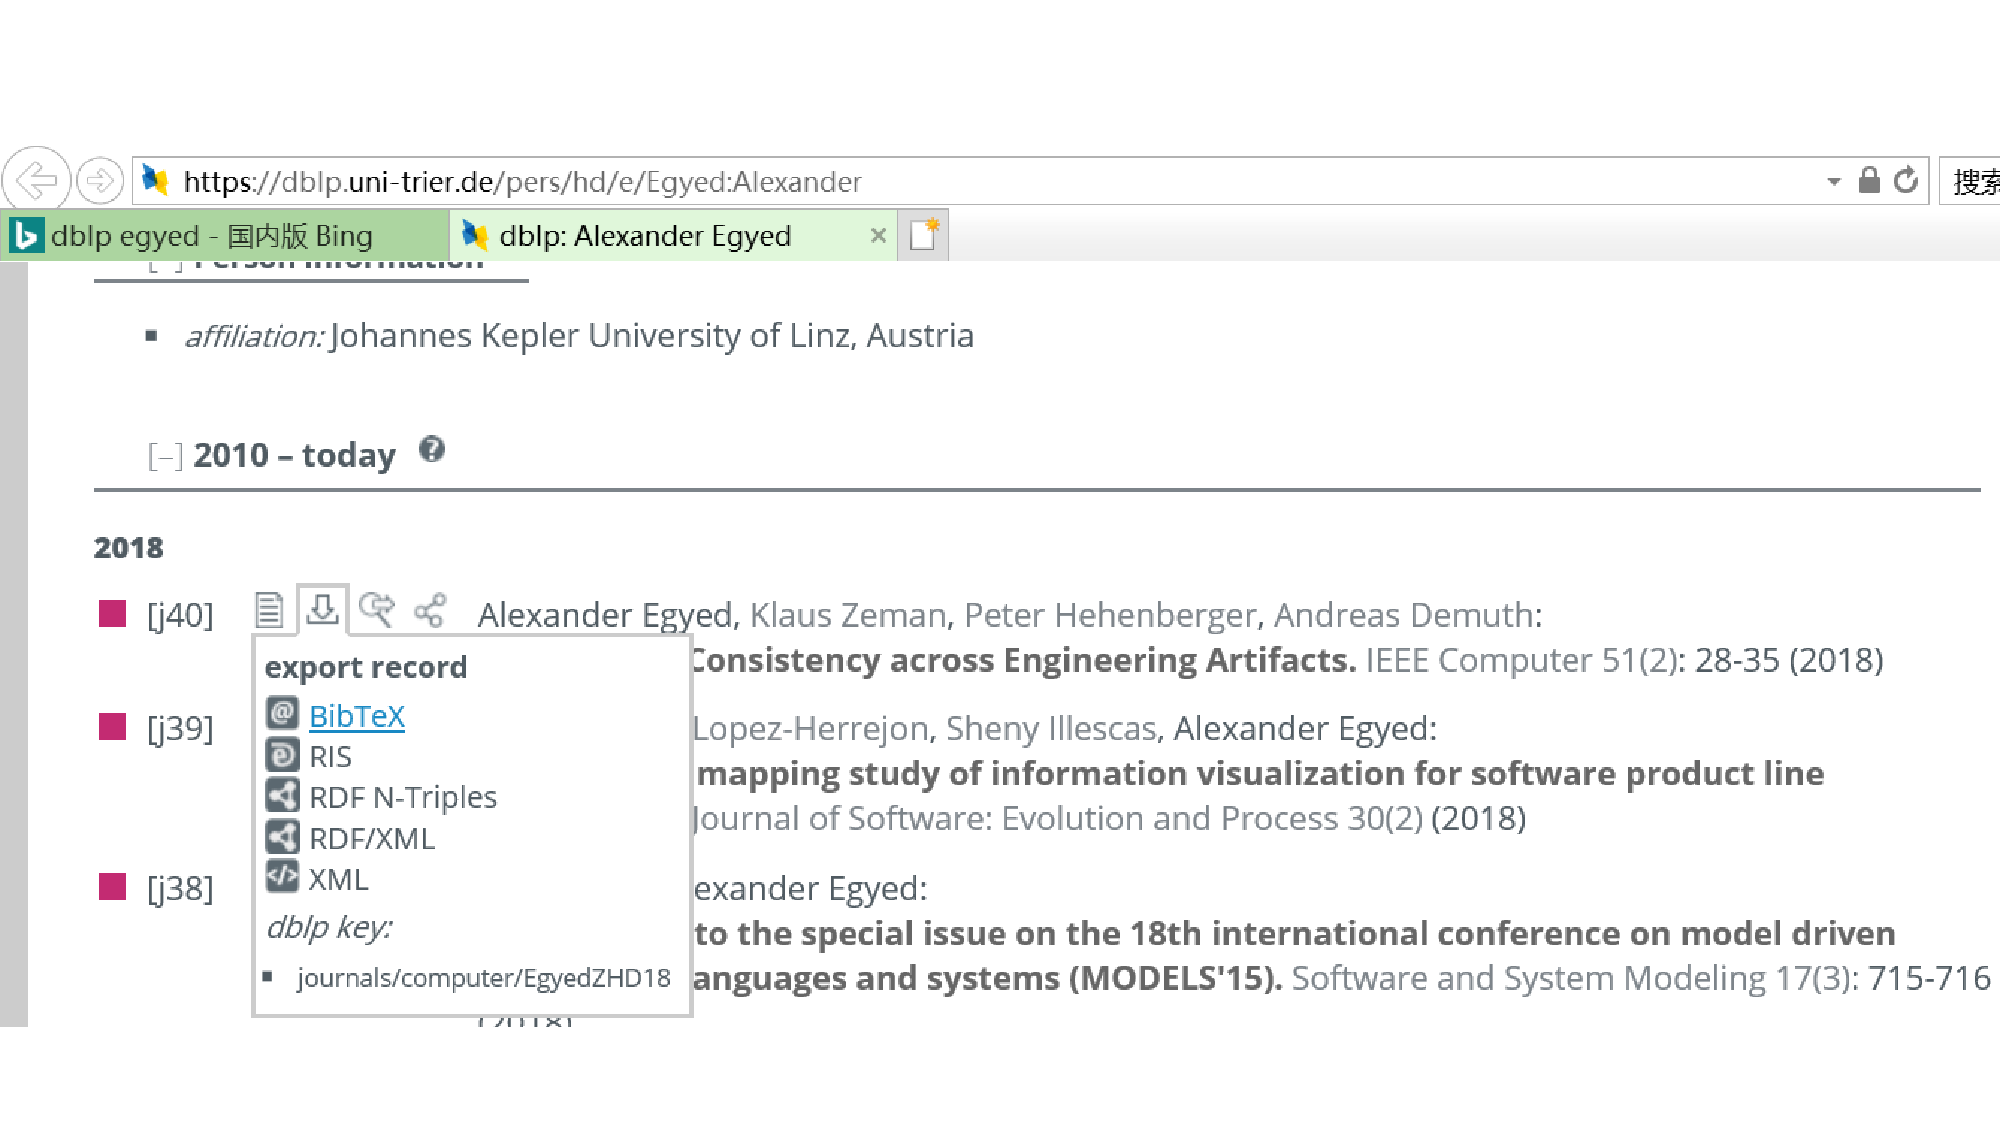
\includegraphics[width=5in]{FIGs/chapter7/dblpForBibtex.pdf}
  \caption{在dblp上下载Bibtex}\label{fig_dblpForBibtexCH7}
\end{figure}

点击该链接之后将得到Bibtex信息,如图~\ref{fig_bibtexDetailCH7}所示。
打开本地文件夹下的reference.bib文件,完整添加该信息。
并在需要引用的位置添加这一引用~\cite{DBLP:journals/computer/EgyedZHD18}。
格式为bibtex信息中的开头,\emph{例如图中的“DBLP:journals/computer/EgyedZHD18”。(此处是一个典型的因为长字符串导致的bad box,请参考上述章节的内容手动完整软换行)}。

\textbf{注意:在修改并保存reference.bib文件后,先点击PDFLaTeX旁边的B按钮编译bib文件,之后需要连续使用PDFLaTeX编译两次,直到最后控制台输出的Warnings不再增加,此时才完成一次论文引用的更新。}

在bib文件中出现,但并未在论文中被引用的论文不会出现在最后的参考文献中。如果dblp中并未包含你需要的论文,则可以尝试谷歌或百度学术的搜索结果,一般也包含bibtex信息,但可能不完整或不规范。

引用网站链接可以考虑这一格式~\cite{GanttSystem}(不推荐,网站链接使用脚注更规范些)。

引用书籍可以考虑这一格式~\cite{Pohl2010Requirements}。

中文文献请参考这一格式~\cite{cyg2006}(引用标记请避免中文,否则容易出现编译错误)。

以下英文引用用来测试引文排序是否按照插入顺序,以及多引文是否合并~\cite{DBLP:journals/computer/EgyedZHD18, DBLP:journals/ml/TingZCZWZ19}

\begin{figure}[htb]
  \centering
  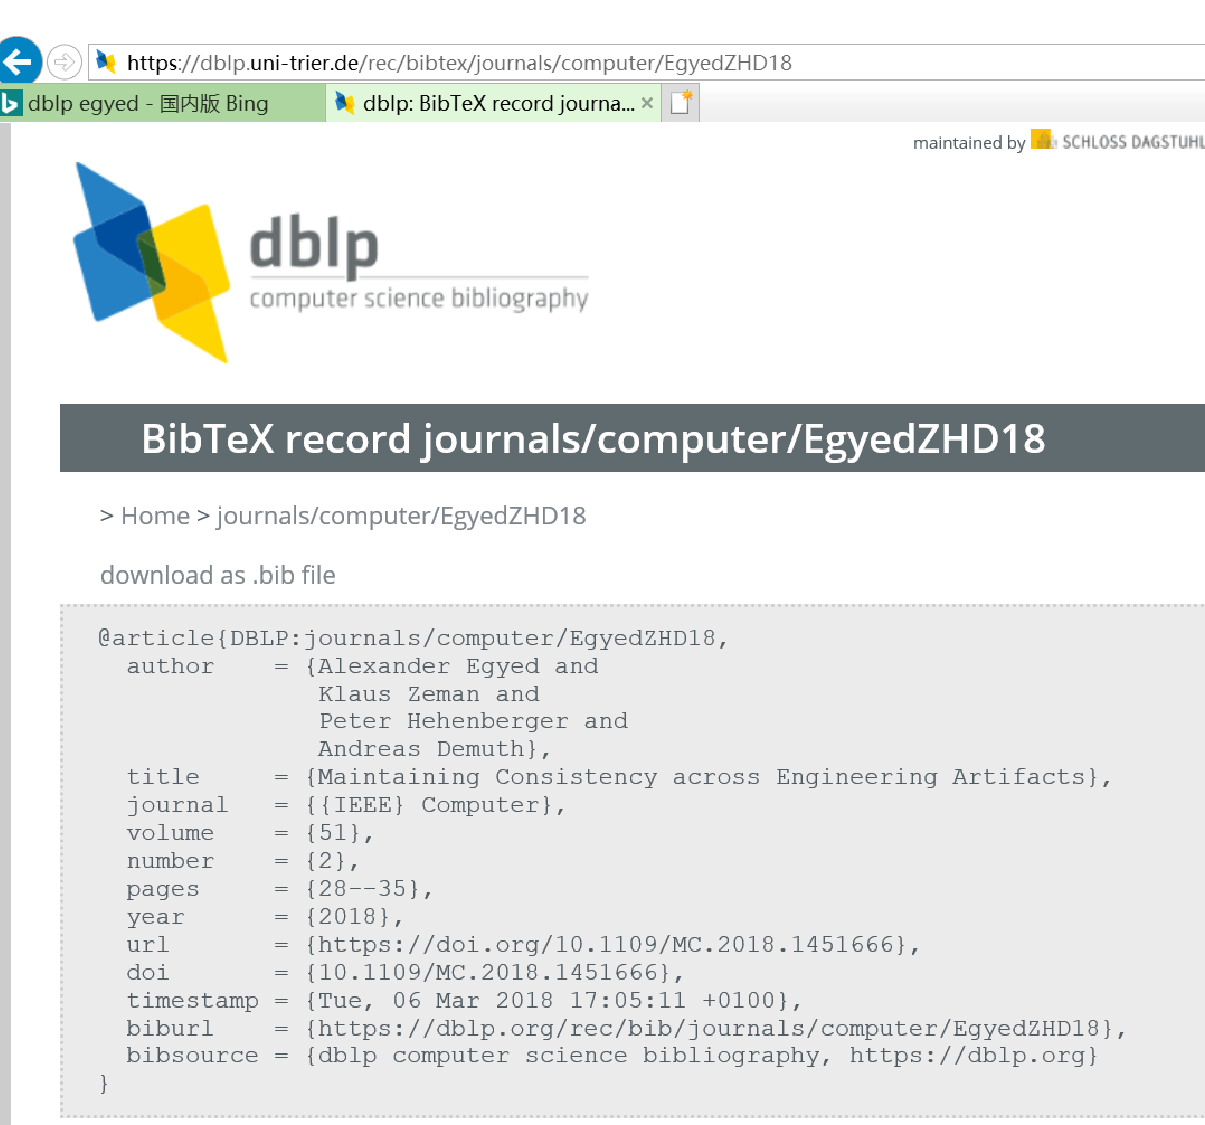
\includegraphics[width=5in]{FIGs/chapter7/bibtexDetail.pdf}
  \caption{Bibtex详细信息}\label{fig_bibtexDetailCH7}
\end{figure}

\section{页眉测试}
以下内容为测试页眉的相关问题、以下内容为测试页眉的相关问题、以下内容为测试页眉的相关问题、以下内容为测试页眉的相关问题、以下内容为测试页眉的相关问题、以下内容为测试页眉的相关问题、

% \chapter{标题}

这是章节标题。
注:一般而言,标题不要比小节标题更小,即不要出现1.2.3.4这种标题(本模板支持此类标题,即Subsubsection)。

\section{这是节标题}

每个章节标题下面都可以插入文字,一般可用于概述下面章节的内容

\subsection{这是小节标题}

此外本模板中的每个章节先保存在独立的tex文件里(本章节文件名为Title.tex,位于本地的chapter文件夹),再通过input命令引入主文件(例如,sample.tex)。
这样做的好处是减少每个文件的行数,便于浏览和维护。
缺点在于有些编辑器编译的时候要求回到主文件进行编译(如WinEdt),或在pdf文件向tex文件跳转的时候定位不准(如TeXStudio)。
如果不能接受上述问题,也可以删除input命令,并将引用文件的全部内容逐一放入主文件。
TeXStudio本身提供对章节索引的管理,可以缓解文件过长的问题。


% \chapter{正文}

需要指出的是本模板使用XeLaTeX编译,要求每个文件都是utf-8编码。
如有使用过CTeX经验的同学,需注意CTeX是使用pdfLaTeX进行编译,并使用GBK编码处理汉字以及CJK(中日韩)字符。
因此,如果要从CTeX源文件复制内容到本模板,必须做编码转化,否则会出现乱码及各种问题。

\section{正文书写的小技巧}
主流的LaTeX编辑器一般都自带一个输出pdf文件查看的功能,并支持在选中文字的区域后跳转到相应的pdf文件或tex文件(所谓的“反复橫跳”),从而尽可能的实现编译后即可得。
以TexStudio为例,在任何一个文件的文字区域点击鼠标右键,即可发现“跳转到源”或者“跳转到pdf”的提示。

只有间隔一个明显的换行才会自然段分段(参见源文件)。

因此,建议把一个自然段中的每句话都单独作为一行。
这样的好处是,每次双击一句话,都可以回到编辑器中具体的一行,方便定位(参见源文件)。

如果觉得TeXStudio自带的pdf查看器不好用,也可以外挂著名的SumatraPDF,并设置正向和反向搜索,能够在论文分章节文件的情况下也做到精准定位(需保持源文件及时更新),具体配置见如下链接 \footnote{https://blog.csdn.net/lizuoxin/article/details/48173907},亲测可行。

注意,配置SumatraPDF时要打开编译过的pdf文件(例如,sample.pdf,会识别出该文件背后存在一个gz文件),才能弹出反向搜索框。而TeXStudio自带的正向搜索命令已失效,要用默认快捷键调出配置中的用户自定义命令。

\section{一些正文中的标记}
\emph{斜体} 与 \textbf{加粗},以及代码格式\texttt{Source Code Pattern}。

\begin{center}
居中,左右对齐同理。
\end{center}

这里再次展示脚注。\footnote{数字列举和圆点列举见摘要部分}

一个小建议,中文后直接跟上述格式标记(包含各种引用)可能会出现一些问题。
因此,在中文字和格式标记的斜杠之间加入~\emph{一个波浪号}是一个常用的习惯。
双~~波~~浪~~线等价于一个强制空格,有时比键盘输入的空格要好用。


\section{注意软换行的使用}
论文一般会引用代码,本模板建议将代码声明为~\texttt{class.this()}格式。
在引用代码时,较长的函数名有时会导致函数名超出文本边界的情况,此时可以考虑手动进行软换行,请参考以下例子。

“图XX 展示了从AquaLush 系统中抽取的函数调用依赖示例,其中~\texttt{UICon-} \linebreak \texttt{troller.buildLogScrn()} 是为了实现新功能“the control panel shows log message”而在新版本中添加的函数。”


% \chapter{表格}

表格是LaTeX中少数没有Word好用的功能。
但word的表格依然存在行间距的问题,而LaTeX也有简洁美观,相对易用(相对)的三线表。

\section{表格与表格引用的基本概念}
表格的编号和表目录都是自动生成并持续编号的,无需人工修改。
只要对表格有标注(label),则在正文中引用该表的label,就可以随时保持最新编号。
此外,表标题一般在表格上方,而图标题一般在图形下方。

\textbf{注意:如果一个新表格加入,并被引用,编辑器将需要连续编译两次到三次,才能完成全部标题、引用和目录的更新。
可以理解为第一次编译引入新表格,此时还不知表格引用位置的具体编号,需要留待第二次编译完成。
而有可能第三次编译才将表格信息写入开头的表目录。
类似的情况也会出现在图形和论文引用这两部分,其中尤以论文引用部分最为奇特,详见最后一章。}

\section{基本表格}

表~\ref{table:codeOverlap}(这里是一个表引用!)是一个简单的三线表,双击表格可以在编辑界面内见到具体设置。

具体解释一下表格的设置:
第一个table体内首先先声明标记位置以及字体大小;
随后声明表格对齐方式;
其次描述表标题;
之后进入具体的表内容(tabular,此时还要声明表格单元中的内容如何对齐);
依次画出三线并填充内容;
如果表格内容较多,可以相应的加入横线来划分(hline);
之后退出tabular;
最后给表起名以实现全局引用,并退出表格。

\begin{table}[htb]\footnotesize
\centering
\caption{实验系统中函数调用与数据依赖的交集}
\vspace{2mm}
% l - left, r - right, c - center. | means one vertical line 这里声明的是表格单元中的内容如何对齐
\begin{tabular}{lccc}
\toprule
&\textbf{Call}&\textbf{Data}&\textbf{Overlap}\\
\midrule
\textbf{VoD}&222&899&66\\
\textbf{GanttProject}&5560&24243&1042\\
\hline
\textbf{jHotDraw}&3943&14555&893\\
\bottomrule
\end{tabular}
\label{table:codeOverlap}
\end{table}

\section{表格单元跨列}

表~\ref{table:codeSmellMethods}展示如何实现表格单元跨列。

\begin{table}[htb]\footnotesize
\centering
\caption{错误率与函数特征之间的关联}
\vspace{2mm}
% l - left, r - right, c - center. | means one vertical line
\begin{tabular}{lcccccc}
\toprule
&\multicolumn{2}{c}{\textbf{Parameters}}
&\multicolumn{2}{c}{\textbf{Return Value}}
&\multicolumn{2}{c}{\textbf{Is Constructor}}\\
&with&without&with&without&with&without\\
\midrule
\textbf{VoD}&8.99\%&9.20\%&6.10\%&9.51\%&9.43\%&8.46\%\\
\textbf{GanttProject}&9.53\%&6.05\%&8.43\%&6.71\%&5.14\%&8.09\%\\
\textbf{jHotDraw}&4.40\%&3.89\%&4.36\%&3.88\%&2.91\%&4.39\%\\
\bottomrule
\end{tabular}
\label{table:codeSmellMethods}
\end{table}

\section{表格单元跨行}

表~\ref{table:systemsCH4}展示如何实现表格单元跨行(Average Number那一行)。
此外,本表格的字体尺寸为scriptsize,比上一个表格的footnotesize要更小。

\begin{table}[htb]\scriptsize
\centering
\caption{五个实验系统概述}
\vspace{2mm}
% l - left, r - right, c - center. | means one vertical line
\begin{tabular}{lccccc}
\toprule
&\textbf{VoD}&\textbf{Chess}&\textbf{GanttProject}&\textbf{jHotDraw}&\textbf{iTrust}\\
\midrule
\textbf{Version}&-&0.1.0&2.0.9&7.2&13.0\\ \hline
\textbf{Programming Language}&Java&Java&Java&Java&Java\\ \hline
\textbf{KLOC}&3.6&7.2&45&72&43\\ \hline
\textbf{Executed methods}&165&316&2741&1755&250\\ \hline
\textbf{Evaluated requirements}&12&7&17&21&34\\ \hline
\multirow{2}{3.5cm}{\textbf{Average Number of Methods Implementing a Requirement}}&45&173&387&121&12\\
&(9-148)&(23-288)&(78-815)&(1-555)&(1-33)\\ \hline
\textbf{Size of the golden RTM}&1980&2212&46597&36855&8500\\ \hline
\textbf{Requirement traces}&534&1210&6584&2547&353\\ \hline
\textbf{Random Chance of guessing}&0.5-7.5\%&1-13\%&0.2-1.7\%&0.003-1.5\%&0.01-0.4\%\\ \hline
\textbf{Method Call Dependencies}&210&439&4830&3848&319\\ \hline
\textbf{Method Data Dependencies}&905&976&30452&17316&5329\\
\bottomrule
\end{tabular}
\label{table:systemsCH4}
\end{table}

\section{表格与图形位置}

常用选项[htbp]是浮动格式:

『h』当前位置。将图形放置在正文文本中给出该图形环境的地方。如果本页所剩的页面不够,这一参数将不起作用。

『t』顶部。将图形放置在页面的顶部。

『b』底部。将图形放置在页面的底部。

『p』浮动页。将图形放置在一只允许有浮动对象的页面上。

 一般使用[htb]这样的组合,只用[h]是没有用的。这样组合的意思就是LaTeX会尽量满足排在前面的浮动格式,就是h-t-b这个顺序,让排版的效果尽量好。图形章节会有更多位置符号的例子。
 
 \section{普通表格(非三线表)}
 
 以下来自于原模板举例的普通表格。
 
 \begin{table}[htbp]
 	\setlength{\belowcaptionskip}{7pt}
 	\centering
 	\caption{编辑距离(乐文斯汀距离计算过程示例表格。字符串``国内企业包括许多''与``国著名括许多''乐文斯汀距离是3)}\label{table:ld}
 	\vspace{0.2cm}
 	\begin{tabular}{|c|c|c|c|c|c|c|c|c|c|}
 		\hline 
 		&   & 国 & 内 & 企 & 业 & 包 & 括 & 许 & 多 \\ 
 		\hline 
 		& 0 & 1 & 2 & 3 & 4 & 5 & 6 & 7 & 8 \\ 
 		\hline 
 		国 & 1 & 0 & 1 & 2 & 3 & 4 & 5 & 6 & 7 \\ 
 		\hline 
 		著 & 2 & 1 & 1 & 2 & 2 & 3 & 4 & 5 & 6 \\ 
 		\hline
 	\end{tabular} 
 \end{table}


% \chapter{图形}

\section{基本图形}
相对于表格而言,LaTeX中的图形就简单多了,需要注意的是本模板推荐将所有图形都转化为pdf,具体内容参见图~\ref{fig_errorExpCH4}。
该图形放在本模板的本地文件夹figure中。
图~\ref{fig_errorExpCH4}是将Excel的五个子图形排布在一个ppt页面上,之后保存为pdf文件,最终得到的图形可以保证是矢量图。


\begin{figure}[htb]
  \centering
  \includegraphics[width=5in]{figure/chapter4/errorExpCH4.pdf}
  \caption{以含错误的RTM为输入的五个系统上三个实验(Call,Data,Call+Data)的错误率(Incorrectness)}\label{fig_errorExpCH4}
\end{figure}

\textbf{注意:不要删除项目下面的njulogo、njuname和reviewPlaceholder这三个文件,分别是论文封面的校徽、手写体南大校名以及盲审时的空白占位符。}

\section{引用代码}

\begin{figure}[htb]
  \centering
  \includegraphics[width=\linewidth]{figure/chapter4/VoDCodeSample.pdf}
  \caption{VoD系统中的代码片段}\label{fig_VoDCodeSample}
\end{figure}

这里给出一个代码引用的推荐实践。
引用代码时先将代码放入word的文本框中,调整结束后,将该文本框页面另存为pdf文件,之后再作为图形来引用,如图~\ref{fig_VoDCodeSample}所示。

\section{其它图引用}

这里给出原模板提供的插图例子,请注意多行多图的设置方式。

一行一图,如图\ref{fig:line}。
\begin{figure}[htbp]
	\centering
	\includegraphics[width=0.7\textwidth]{figure/line.png} % requires the graphicx package
	\caption{待分行文本}
	\label{fig:line}
	%\vspace{0.8cm} % 用来调整和下方文字的间距
\end{figure}


一行两个图,如图\ref{fig:lstm}。
\begin{figure}[ht!]
	\centering
	\begin{subfigure}{.5\textwidth}
		\centering
		\includegraphics[width=0.9\textwidth]{figure/lstm1.png}
		\caption{长短时记忆单元模块}
	\end{subfigure}
	\begin{subfigure}{.4\textwidth}
		\centering
		\includegraphics[width=0.8\textwidth]{figure/lstm2.png}
		\caption{深双向长短时记忆}
		\label{fig:lstm2}
	\end{subfigure}
	\caption{(a)一个长短时记忆单元模块。(b)深度双向长短时记忆的结构。}
	\label{fig:lstm}
\end{figure}

多行多图,如图\ref{fig:multi}。注意源文件中的双空行起到了子图换行的作用。
子图中大小不一是有意为之,请留意源码中subfigure和includegraphics后面的命令与四个子图大小之间的关系。

\textbf{注意:后续连续出现图形是最终文档中需要避免的情况,一般而言出现这种情况都是图贴的太多,文字写的太少导致的。建议针对每个图或表都采用“三段论”,即给出图表之前先介绍图表的大致情况与理由,然后给出图表,在图表展示之后再对图表中的内容进行讨论。}

\begin{figure}[ht!]
	\centering
	\begin{subfigure}{.69\textwidth}
		\centering
		\includegraphics[width=1.0\textwidth]{figure/line1.png}
		\caption{全局损失切割第一行}
		\label{fig:line1}
	\end{subfigure}
	\begin{subfigure}{.3\textwidth}
		\centering
		\includegraphics[width=1.0\textwidth]{figure/line2.png}
		\caption{局部损失切割第一行}
		\label{fig:line2}
	\end{subfigure}
	
	
	\begin{subfigure}{.49\textwidth}
		\centering
		\includegraphics[width=0.5\textwidth]{figure/line1.png}
		\caption{全局损失切割第二行}
		\label{fig:line1}
	\end{subfigure}
	\begin{subfigure}{.49\textwidth}
		\centering
		\includegraphics[width=0.8\textwidth]{figure/line2.png}
		\caption{局部损失切割第二行}
		\label{fig:line2}
	\end{subfigure}
	\caption{分行结果比较。(a)全局损失切割;(b)局部损失切割;(c)缩放的全局损失切割;(d)缩放的局部损失切割}
	\label{fig:multi}
\end{figure}

\newpage %为了将图片实例放在一起,另起一页,使用时请删掉




% \chapter{公式}

这里直接给出几个较为复杂的公式的例子,可一一进行参照。
若有未包含的数学符号或公式格式,请参阅本模板所包含的手册(本地manual文件夹)或百度必应谷歌。
介绍公式时不妨也采用下面的方式,即先介绍公式的目的,给出公式,并逐一介绍公式中的变量。

\section{公式5.1与论证}
“从直接代码依赖的角度出发,从一个初始域外的类$C_{out}$ 出发我们尝试找到一个通往初始域内的类$C_{in}$ 的路径。一条合法的路径需要满足以下两点要求:(1)这一路径是单向的,即$C_{out}$ 传递性地到达$C_{in}$ 或$C_{in}$ 传递性地到达$C_{out}$;(2)路径中只能包含一个$C_{in}$ (为了避免重复路径的出现)。为了恰当的估计一条合法路径所代表的交互程度,我们计算路径上所有直接代码依赖的紧密度值的几何平均。我们用如下公式来重新计算给定$C_{out}$ 的IR 值($IR_{DC}$):”

\begin{align}
IR_{DC}=IR_{origin}+(IR_{top}-IR_{origin})^{\left| PATH\right|}\sqrt {\prod _{x \in PATH}Closeness_{DC}(x)} \end{align}

“其中$IR_{origin}$ 代表$C_{out}$ 的初始IR值,$IR_{top}$ 代表$C_{in}$ 被提升过的IR值,\emph{PATH} 代表$C_{out}$ 与$C_{in}$ 之间的路径内所有的直接代码依赖,而$Closeness_{DC}(x)$ 则代表每一条直接代码依赖关系的紧密度值。在同一对$C_{out}$ 和$C_{in}$ 之间可能存在多条合法路径,我们只保留其中能使$IR_{DC}$ 值最大的那条路径。”

\section{公式5.2与论证}

“由于IR 方法返回的是一个按照IR 值大小倒序排列的候选线索列表,因此一种常用的比较IR 方法的方式是在不同的查全率水平上比较不同方法之间的精确度,通常用$Precision-Recall$ 曲线表示。为了进一步衡量IR 方法返回结果的整体质量,我们选用了另外两个常用的实验度量:$AP$(Average Precision)与$MAP$ (Mean Average Precision)。其中,$AP$ 用于度量全部查询(需求)所检索的相关文档的排序质量,计算方式如下:”
\begin{align}
AP=\dfrac {\sum _{r=1}^{N}\left( Precision\left( r\right) \times isRelevant\left( r\right) \right) } {\left| RelevantDocuments\right| }
\end{align}

“其中,$r$ 表示被查询对象(类)在列表中的排序,$Precision(r)$ 表示前$r$ 个类的准确率。$isRelevant()$ 为一个二值函数,如果文档是相关的,则返回1,若无关,则返回0。”

\section{公式5.3与论证}

“由此,我们为类数据依赖定义紧密度$Closeness_{CD}$ 如下:”

\begin{align}Closeness_{CD}=\frac {\sum _{x \in \{DT_{i}\cap DT_{j}\}}idtf(x)} {\sum _{y \in \{DT_{i}\cup DT_{j}\}}idtf(y)}\end{align}

“其中$idtf(x)$ 代表共享数据类型的idtf值,$DT_i$ 与$DT_j$ 的交集代表该数据依赖上的共享数据类型,而$DT_i$ 与$DT_j$ 的并集则代表$C_i$ 和$C_j$ 在全部代码上所访问的数据类型。$Closeness_{CD}$ 的取值范围是0到1之间。”

\section{原模板中的其它公式}

\begin{equation}
\frac{\partial L}{\partial a_{k}^t} = {d(s)}^2 (y_{k}^t - \frac{\sum_{lab(\mathbf{l},k)} \alpha_t(s)\beta_t(s) }{y_{k}^t} )
\end{equation}

\begin{equation}
\begin{aligned}
d_{{0j}}&=\sum _{{k=1}}^{{j}}w_{{\mathrm  {ins}}}(a_{{k}}),\quad &{\text{for}}\;1\leq j\leq n\\
d_{{ij}}&={\begin{cases}d_{{i-1,j-1}}&{\text{for}}\;a_{{j}}=b_{{i}}\\\min {\begin{cases}d_{{i-1,j}}+w_{{\mathrm  {del}}}(b_{{i}})\\d_{{i,j-1}}+w_{{\mathrm  {ins}}}(a_{{j}})\\d_{{i-1,j-1}}+w_{{\mathrm  {sub}}}(a_{{j}},b_{{i}})\end{cases}}&{\text{for}}\;a_{{j}}\neq b_{{i}}\end{cases}}\quad &{\text{for}}\;1\leq i\leq m,1\leq j\leq n.
\end{aligned}
\end{equation}

\begin{equation}
\begin{aligned}
&\beta_T(|l{}'|)=y_{b}^{T}\\
&\beta_T(|l{}'|-1)=y_{l_|l|}^{T} \\
&\beta_T(s)=0, \forall s < |l{}'|-1
\end{aligned}
\end{equation}

递归公式举例(出现了公式过长的问题,实践中最好适当控制长度,给公式编号在同一行上留下位置)。
\begin{equation}
\beta_t(s)=\left\{
\begin{aligned}
& (\beta_{t+1}(s) d(s)+\beta_{t+1}(s+1))d(s+1)\,  y_{\l_s{}'}^t, \: \: if \:  l_s{}'=b \:  or \:  l_{s+2}{}'=l_s{}'\\
& (\beta_{t+1}(s) d(s)+\beta_{t+1}(s+1)d(s+1)+\beta_{t+1}(s+2)d(s+2))\,  y_{\l_s{}'}^t,\: \:   otherwise
\end{aligned}
\right.
\end{equation}



% \chapter{论文引用}

\section{引文相关}
此处的论文引用采用的是类似于IEEE的按出现位置的数字编号格式。建议将被引用的论文全名放入dblp网站(必应谷歌搜索dblp)搜索,之后进入该论文详细信息,如图~\ref{fig_dblpForBibtexCH7} 所示。

\begin{figure}[htb]
  \centering
  \includegraphics[width=5in]{figure/chapter7/dblpForBibtex.pdf}
  \caption{在dblp上下载Bibtex}\label{fig_dblpForBibtexCH7}
\end{figure}

点击图~\ref{fig_dblpForBibtexCH7}中所示的链接之后将得到Bibtex信息,如图~\ref{fig_bibtexDetailCH7}所示。
打开本地文件夹下的sample.bib文件,完整添加该信息。
并在需要引用的位置添加这一引用~\cite{DBLP:journals/computer/EgyedZHD18}。
格式为bibtex信息中的开头,\emph{例如图中的“DBLP:journals/computer/EgyedZHD18”。(此处是一个典型的因为长字符串导致的bad box,请参考上述章节的内容手动进行软换行)}。

\textbf{注意:在修改并保存sample.bib文件后,先编译tex文件,再编译参考文献,之后再编译两次,此时引用位置的方括号内将出现具体的编号而不是问号,且编号对应的引文已经出现在参考文献内。本模板点击引用编号后可以跳转到对应的参考文献处。}

在bib文件中出现,但并未在论文中被引用的论文不会出现在最后的参考文献中。如果dblp中并未包含你需要的论文,则可以尝试谷歌或百度学术的搜索结果,一般也包含bibtex信息,但可能不完整或不规范。

引用网站链接可以考虑这一格式~\cite{GanttSystemWeb}(不推荐,网站链接使用脚注更规范些)。

引用书籍可以考虑这一格式~\cite{Pohl2010Requirements}。

中文文献请参考这一格式~\cite{cyg2006}(引用标记不要使用中文,否则容易出现编译错误)。

以下英文引用用来测试引文排序是否按照插入顺序,以及多引文是否合并~\cite{DBLP:journals/computer/EgyedZHD18, DBLP:journals/ml/TingZCZWZ19}

\begin{figure}[htb]
  \centering
  \includegraphics[width=5in]{figure/chapter7/bibtexDetail.pdf}
  \caption{Bibtex详细信息}\label{fig_bibtexDetailCH7}
\end{figure}


%%%%%%%%%%%%%%%%%%%%%%%%%%%%%%%%%%%%%%%%%%%%%%%%%%%%%%%%%%%%%%%%%%%%%%%%%%%%%%%
% 致谢,应放在结论之后
\begin{acknowledgement}
在本篇论文最后,我想真诚地感谢在我撰写论文过程中指导和帮助我的老师、同学们,
还有支持我、鼓励我的家人和朋友们。

首先,我要感谢在我毕设研究工作中,张贺教授对我的悉心指导和帮助,
在跟随您的两年研究生学习工作中,您总是教导我们要多去实践,
要以严谨认真的态度踏踏实实地完成科研学习工作,
还要努力阅读大量学术文献,提高自己看问题的层次,
还为我们提供了很多与工业界交流的机会,这些都为我的毕设工作和日常工作学习带来了很大的好处。

然后,我要感谢实验室的师兄师姐和同学们,
感谢你们这两年中在学习、工作和生活中带给我的帮助与鼓励,
特别是指导我毕设工作的师姐,对我的问题一一解答,对我的论文工作耐心指导,
启发我进行深度的思考,反复与我评估和讨论论文研究的问题,
得益于她的帮助,我的论文才能保质保量地顺利完成。

最后,还要感谢我的父母和家人,感谢你们在背后默默支持和陪伴我。
很幸运,在研究生阶段遇到了相互扶持,互相鼓励的伴侣,
在生活和学习上我们互相帮助,给予彼此很大的动力与希望。
也要感谢我的舍友们,让我的生活中充满了乐趣。

在论文工作中,访谈和焦点小组中付出了大量的精力时间,
实现工具时也遇到过困难与问题,但我依然坚持尽力做到最好,
马上就要从学校步入社会,我将坚持“诚朴雄伟,励学敦行”的精神,
不畏艰难,努力奋斗出属于自己的一片天地。
  
\end{acknowledgement}




% 参考文献。应放在\backmatter之前。
% 推荐使用BibTeX,若不使用BibTeX时注释掉下面一句。
%\nocite{*}
\bibliography{sample}


% 附录,必须放在参考文献后,backmatter前
\appendix
\chapter{访谈问题}\label{app:1}
\section{战术建模访谈问题}

\noindent 一、个人信息

\noindent 1.您的职位是?

\noindent
A.开发人员

\noindent
B.	架构师

\noindent
C.	项目管理者

\noindent
D.	运维人员

\noindent
E.	其他

\noindent
2.	您所在团队的人员规模?

\noindent
A.		5人以下

\noindent
B.	5-10人

\noindent
 C.	10-20人

\noindent
 D.	20-50人

\noindent
 E.	50人以上

\noindent
 3.	您所在团队业务关注的领域?

\noindent
A.	软件/IT领域

\noindent
B.	通信领域

\noindent
C.	软件提供商

\noindent
D.	电商领域

\noindent
E.	银行和金融领域

\noindent
F.	其他

\noindent
二、	DDD建模总体实践

\noindent
1.	您的团队按照领域驱动设计进行领域建模的流程是什么?

\noindent
a)	分析建模、设计建模和实现建模的顺序

\noindent
b)	领域模型图和代码实现之间的关系

\noindent
2.	您的团队是否有使用某种建模工具进行领域建模?是什么建模工具?它的优缺点是什么? 

\noindent
a)	DDD专用的建模套件工具

\noindent
b)	传统的类图工具,如EA、PlantUML、visual paradigm

\noindent
c)	使用纸和笔直接进行建模

\noindent
三、	DDD战术建模模式实践

\noindent
1.	关于实体

\noindent
a)	您认为何时应该使用实体?

\noindent
b)	您认为实体应该包含哪些重要属性?

\noindent
i.	实体应该拥有唯一标识,方便跟踪和与其他实体区分

\noindent
ii.	实体在其生命周期内可以连续变化

\noindent
c)	除上述属性外,还应该包括哪些属性?

\noindent
d)	您的团队在实现实体时有哪些最佳实践?

\noindent
i.	如何建模唯一标识

\noindent
ii.	唯一标识通常由哪些组成部分

\noindent
iii.	如何为标识生成唯一值,即如何生成唯一标识

\noindent
iv.	什么时候生成唯一标识

\noindent
v.	如何存储唯一标识

\noindent
vi.	如何保证唯一标识的稳定性

\noindent
e)	您认为在建模实体时有哪些不好的实践是需要避免的?

\noindent
2.	关于值对象

\noindent
a)	您认为何时应该使用值对象?

\noindent
b)	您认为值对象应该包含哪些重要属性?

\noindent
i.	不变性

\noindent
ii.	可替换性

\noindent
iii.	值对象相等性

\noindent
iv.	无副作用行为

\noindent
v.	是一个概念整体

\noindent
c)	除上述属性外,还应该包括哪些属性?

\noindent
d)	您的团队在实现值对象时有哪些最佳实践?

\noindent
i.	如何保证值对象的不可变性

\noindent
ii.	如何实现无副作用行为

\noindent
iii.	如何存储值对象集合

\noindent
e)	您认为在建模值对象时有哪些不好的实践是需要避免的?

\noindent
3.	关于服务

\noindent
a)	您认为何时应该使用服务?

\noindent
b)	您认为领域服务应该包含哪些重要属性?

\noindent
i.	无状态

\noindent
c)	除上述属性外,还应该包括哪些属性?

\noindent
d)	您的团队在实现领域服务时有哪些最佳实践?

\noindent
i.	如何组织领域服务,领域服务放在项目中的什么位置

\noindent
e)	您认为在建模领域服务时有哪些不好的实践是需要避免的?

\noindent
4.	关于领域事件

\noindent
a)	您认为何时应该使用领域事件?

\noindent
b)	您认为领域事件应该具有哪些属性

\noindent
i.	事件发生时间

\noindent
ii.	事件的发送方或造成事件的对象

\noindent
iii.	不变性

\noindent
iv.	唯一标识

\noindent
c)	除上述属性外,还应该包括哪些属性?

\noindent
d)	是否应该将领域事件建模成聚合?

\noindent
e)	您的团队在实现领域事件时有哪些最佳实践?

\noindent
i.	如何命名领域事件

\noindent
ii.	如何存储事件发生的时间

\noindent
iii.	如何保证领域事件的不变性

\noindent
iv.	如何避免将领域模型暴露给消息设施

\noindent
v.	如何保证在事件发布前完成订阅

\noindent
vi.	如何保证领域模型和事件存储的一致性

\noindent
vii.	存储的领域事件有何作用

\noindent
viii.	如何转发领域事件

\noindent
ix.	何时应该把领域事件建模成聚合

\noindent
f)	您认为在建模领域事件时有哪些不好的实践是需要避免的?

\noindent
5.	关于模块

\noindent
a)	您认为何时应该使用模块?

\noindent
b)	您认为模块应该具有哪些属性?

\noindent
c)	您的团队在实现模块时有哪些最佳实践?

\noindent
i.	如何命名模块

\noindent
ii.	模块的表现形式,Java中的包,C++命名空间

\noindent
iii.	如何组织模块

\noindent
d)	您认为在建模模块时有哪些不好的实践是需要避免的?

\noindent
6.	关于聚合

\noindent
a)	您认为何时应该使用聚合?

\noindent
b)	您认为聚合应该包含哪些重要属性?

\noindent
i.	边界内保持一致性

\noindent
ii.	根实体

\noindent
iii.	值对象/其他实体

\noindent
c)	除上述属性外,还应该包括哪些属性?

\noindent
d)	您的团队在实现聚合时有哪些最佳实践?

\noindent
i.	如何设计一个聚合

\noindent
ii.	聚合中如何使用其他聚合或对象(对象的导航性)

\noindent
iii.	如何保证一致性边界

\noindent
iv.	何时允许在单个事务中修改多个聚合

\noindent
v.	如何隐藏聚合内部信息

\noindent
vi.	如何引用其他聚合

\noindent
e)	您认为在建模聚合时有哪些不好的实践是需要避免的?

\noindent
7.	关于资源库

\noindent
a)	您认为何时应该使用资源库?

\noindent
b)	您认为资源库应该具有哪些属性?

\noindent
i.	只为聚合提供资源库(一种和其他pattern的关系,能否算作属性)

\noindent
c)	您的团队在实现资源库时有哪些最佳实践?

\noindent
i.	如何设计资源库,面向集合还是面向持久化

\noindent
d)	资源库经常与聚合相关,是否应该将领域对象的关联关系作为属性?

\noindent
e)	您认为在建模资源库时有哪些不好的实践是需要避免的?


\noindent
8.	关于工厂

\noindent
a)	您认为何时应该使用工厂?

\noindent
i.	委托其他对象创建复杂对象对性能的影响可以忽略时

\noindent
ii.	需要减轻客户端在创建聚合实例的负担

\noindent
iii.	确保创建实例处于正确状态时

\noindent
b)	您认为工厂应该具有哪些属性?

\noindent
c)	您的团队在实现工厂时有哪些最佳实践?

\noindent
i.	工厂应该放在何处,作为聚合的一部分还是独立成领域服务

\noindent
d)	您认为在建模工厂时有哪些不好的实践是需要避免的?


%%%%%%%%%%%%%%%%%%%%%%%%%%%%%%%%%%%%%%%%%%%%%%%%%%%%%%%%%%%%%%%%%%%%%%%%%%%%%%%
% 书籍附件
\backmatter
%%%%%%%%%%%%%%%%%%%%%%%%%%%%%%%%%%%%%%%%%%%%%%%%%%%%%%%%%%%%%%%%%%%%%%%%%%%%%%%
% 作者简历与科研成果页,应放在backmatter之后
\begin{resume}
% 论文作者身份简介,一句话即可。
\begin{authorinfo}
\noindent 李质颖,男,汉族,1997年2月出生,山东省济宁人。
\end{authorinfo}
% 论文作者教育经历列表,按日期从近到远排列,不包括将要申请的学位。
\begin{education}
\item[2015年9月 --- 2019年6月] 重庆大学大数据与软件学院 \hfill 本科
\end{education}
% 论文作者在攻读学位期间所发表的文章的列表,按发表日期从近到远排列。
% \begin{publications}
% \item Fuli Zhang, Peiyu Hou,  ``一种智能合约微服务化框架'' 
%   in \textsl{Proc. IEEE International Conference on Communications (ICC) 2010}, May. 2010.
% \end{publications}
% 论文作者在攻读学位期间参与的科研课题的列表,按照日期从近到远排列。
% \begin{projects}
% % \item 国家自然科学基金面上项目``问题研究''
% % (课题年限~2010年1月 --- 2012年12月),负责相关问题的研究。
% \end{projects}
\end{resume}

%%%%%%%%%%%%%%%%%%%%%%%%%%%%%%%%%%%%%%%%%%%%%%%%%%%%%%%%%%%%%%%%%%%%%%%%%%%%%%%
% 生成《学位论文出版授权书》页面,应放在最后一页
%\makelicense

%%%%%%%%%%%%%%%%%%%%%%%%%%%%%%%%%%%%%%%%%%%%%%%%%%%%%%%%%%%%%%%%%%%%%%%%%%%%%%%
\end{document}
